\documentclass[13pt,a4paper]{report}

% ==================== XỬ LÝ FONT TIẾNG VIỆT CHỐNG LỖI ====================
\usepackage{iftex}
\ifPDFTeX
  % Cấu hình chuẩn cho trình biên dịch pdfLaTeX (phổ biến nhất trên Overleaf)
  \usepackage[utf8]{inputenc}
  \usepackage[T5]{fontenc}        % Bảng mã T5 chuẩn cho tiếng Việt đầy đủ dấu
  \usepackage[vietnamese]{babel}
  \usepackage{mathptmx}           % Font Times New Roman tương thích pdfLaTeX
\else
  % Cấu hình chuẩn cho trình biên dịch XeLaTeX hoặc LuaLaTeX
  \usepackage{fontspec}
  \usepackage[vietnamese]{babel}
  \setmainfont{Times New Roman}[
      BoldFont = * Bold,
      ItalicFont = * Italic,
      BoldItalicFont = * Bold Italic
  ]
\fi

% ==================== CĂN LỀ & KHUNG TRANG CHUẨN ====================
\usepackage{geometry}
\geometry{
    a4paper,
    top=20mm,
    bottom=20mm,
    left=30mm,
    right=20mm
}
\usepackage{setspace}
\setstretch{1.15} % Chuẩn giãn dòng 1.15
\setlength{\parindent}{0.8cm}
\setlength{\parskip}{3pt}
\tolerance=1200
\emergencystretch=1.5em
\hbadness=2000
\raggedbottom

% ==================== GÓI ĐỒ HỌA, BẢNG BIỂU & HÌNH ẢNH ====================
\usepackage{graphicx}
\usepackage{tikz}
\usetikzlibrary{calc}
\usepackage{booktabs}
\usepackage{tabularx}
\usepackage{array}
\usepackage{amsmath,amssymb}
\usepackage{caption}
\captionsetup[table]{name=Bảng, font=small, labelfont=bf, skip=6pt}
\captionsetup[figure]{name=Hình, font=small, labelfont=bf, skip=6pt}
\usepackage{needspace}
\usepackage{placeins}
\renewcommand{\topfraction}{0.85}
\renewcommand{\bottomfraction}{0.85}
\renewcommand{\textfraction}{0.10}
\renewcommand{\floatpagefraction}{0.80}

% ==================== ĐỊNH DẠNG HEADER / FOOTER & LINK ====================
\usepackage{fancyhdr}
\usepackage{xcolor}
\usepackage{tcolorbox}
\tcbuselibrary{breakable}
\tcbset{
    sqlblock/.style={
        breakable,
        colback=gray!6,
        colframe=blue!40!black!45,
        boxrule=0.6pt,
        arc=2pt,
        left=8pt,
        right=8pt,
        top=5pt,
        bottom=5pt,
        before skip=6pt,
        after skip=6pt
    }
}
\PassOptionsToPackage{hyphens}{url}
\usepackage{hyperref}
\hypersetup{
    colorlinks=true,
    linkcolor=black,
    citecolor=blue!70!black,
    urlcolor=blue!70!black
}


% Định dạng tiêu đề chương và mục
\usepackage{titlesec}
\titleformat{\chapter}[block]
  {\normalfont\bfseries\Large\centering}{CHƯƠNG \thechapter.}{0.5em}{}
\titlespacing*{\chapter}{0pt}{-14pt}{12pt}

\titleformat{\section}
  {\normalfont\bfseries\large}{\thesection.}{0.5em}{}
\titlespacing*{\section}{0pt}{10pt}{5pt}

\titleformat{\subsection}
  {\normalfont\bfseries\normalsize}{\thesubsection.}{0.5em}{}
\titlespacing*{\subsection}{0pt}{8pt}{4pt}

% ==================== BẮT ĐẦU TÀI LIỆU ====================
\begin{document}
% -------------------- TRANG BÌA CHUẨN UET --------------------
\begin{titlepage}
    % Vẽ khung viền kép trang bìa bằng TikZ
    \begin{tikzpicture}[remember picture, overlay]
        \draw[line width = 2pt, color = blue!80!black]
            ($(current page.north west) + (20mm,-15mm)$)
            rectangle
            ($(current page.south east) + (-15mm,15mm)$);
        \draw[line width = 0.75pt, color = blue!80!black]
            ($(current page.north west) + (21.5mm,-16.5mm)$)
            rectangle
            ($(current page.south east) + (-16.5mm,16.5mm)$);
    \end{tikzpicture}

    \begin{center}
        {\large \textbf{ĐẠI HỌC QUỐC GIA HÀ NỘI}}\\[0.2cm]
        {\large \textbf{TRƯỜNG ĐẠI HỌC CÔNG NGHỆ}}\\[0.8cm]

        % Chèn logo UET (nếu có file uet_logo.png thì hiển thị, nếu chưa upload thì hiển thị khung giả lập)
        \IfFileExists{uet_logo.png}{
            \includegraphics[width=4.2cm]{uet_logo.png}\\[0.8cm]
        }{
            \begin{tikzpicture}
                \draw[blue!70!black, fill=blue!5] (0,0) circle (1.8cm);
                \node at (0,0) [align=center, blue!80!black, font=\bfseries\small] {LOGO UET\\(uet\_logo.png)};
            \end{tikzpicture}\\[0.8cm]
        }

        {\Large \textbf{BÁO CÁO HỌC PHẦN}}\\[0.3cm]
        {\LARGE \textbf{HỆ QUẢN TRỊ CƠ SỞ DỮ LIỆU}}\\[0.6cm]

        \rule{8cm}{0.4pt}\\[0.8cm]

        {\large \textbf{ĐỀ TÀI:}}\\[0.5cm]
        {\Large \textbf{CLICKHOUSE VÀ ĐỘNG CƠ LƯU TRỮ MERGETREE: KIẾN TRÚC LÕI, ĐỐI SÁNH ĐA HỆ QUẢN TRỊ CSDL VÀ ỨNG DỤNG PHÂN TÍCH CLICKSTREAM THỜI GIAN THỰC}\par}
        \vspace{1.0cm}

        \begin{flushleft}
            \normalsize
            \hspace*{2.2cm}\textbf{Lớp học phần:} INT3202\_I (Hệ quản trị Cơ sở dữ liệu -- DBMS)\\[0.25cm]
            \hspace*{2.2cm}\textbf{Giảng viên hướng dẫn:} ThS. Nguyễn Thị Cẩm Vân \\[0.25cm]
            \hspace*{2.2cm}\textbf{Nhóm thực hiện:} Nhóm 8\\[0.25cm]
            \hspace*{3.5cm}\begin{tabular}{@{}l@{\hspace{0.8cm}}l@{}}
                24020303 & Võ Anh Tài \\
                24020348 & Võ Hoài Anh Tuấn \\
                24020115 & Nguyễn Thị Ngọc Hà
            \end{tabular}
        \end{flushleft}

        \vfill
        {\large \textbf{Hà Nội, Tháng 11 / 2026}}
    \end{center}
\end{titlepage}

% -------------------- PHẦN ĐẦU (ĐÁNH SỐ TRANG LA MÃ) --------------------
\pagenumbering{roman}
\setcounter{page}{1}

% Thiết lập Header cho các trang nội dung
\pagestyle{fancy}
\fancyhf{}
\fancyhead[L]{\small\textit{Báo cáo nghiên cứu: Hệ quản trị cơ sở dữ liệu (INT3202)}}
\fancyhead[R]{\small\textit{Nhóm 8 (Hà -- Tuấn -- Tài) - 2026}}
\fancyfoot[C]{\thepage}
\renewcommand{\headrulewidth}{0.4pt}

% --- MỤC LỤC ---
{\setstretch{1.00}\setlength{\parskip}{0pt}
\tableofcontents
}
\clearpage

% --- TÓM TẮT ---
\phantomsection
\addcontentsline{toc}{chapter}{Tóm tắt báo cáo (Abstract)}
\begin{center}
    {\Large\textbf{TÓM TẮT BÁO CÁO (ABSTRACT)}}
\end{center}
\vspace{0.25cm}

Báo cáo nghiên cứu toàn diện về \textbf{ClickHouse} --- hệ quản trị cơ sở dữ liệu phân tích hướng cột (\textit{Columnar OLAP DBMS}) mã nguồn mở hiệu năng cao --- xoay quanh 3~trụ cột: \textbf{(1)}~làm rõ kiến trúc DBMS hoàn chỉnh cùng triết lý \textit{hardware-sympathetic} và giải phẫu điểm sáng cốt lõi \textbf{MergeTree}; \textbf{(2)}~đối chiếu cơ chế điểm sáng MergeTree với các họ DBMS hiện đại (PostgreSQL, RocksDB/Cassandra, Apache Druid/Pinot, Elasticsearch, DuckDB) kèm thực nghiệm đối chứng trực diện trên 30~triệu dòng với PostgreSQL~18.6; và \textbf{(3)}~vận dụng chính các điểm sáng của MergeTree để giải quyết bài toán phân tích luồng nhấp chuột (\textit{clickstream}) cường độ 10.000~sự kiện/giây (bổ sung đối chứng cùng hệ cột với DuckDB~2.0.1 và kiểm chứng Skipping Index, Projection, External Spill, hợp nhất qua ngưỡng Wide Part và \texttt{ReplacingMergeTree FINAL} trực tiếp trên \texttt{laptop1}).

\begin{itemize}
    \setlength{\itemsep}{2pt}
    \setlength{\parskip}{0pt}
    \setlength{\parsep}{0pt}
    \item \textbf{Kiểm chứng nội tại MergeTree (E1--E3, 30M~dòng ClickBench \texttt{hits}, kiểm định Mann--Whitney~U):} (i)~đặt đúng tiền tố \texttt{ORDER BY} cắt tỉa tới 99,95\% hạt dữ liệu và tăng tốc tới 7,76${\times}$ ($p = 0{,}00002$), trong khi chỉ mục chính thưa trong RAM chỉ tốn 21.978~B ($\approx 21{,}46~\text{KiB}$, khớp 0,00\% sai số giải tích) và \texttt{SerializationSparse} tự động cắt giảm $\approx 114{,}3~\text{MB}$ chưa nén; (ii)~ở bảng hẹp 44~B/dòng, \texttt{index\_\allowbreak{}granularity = 8192} giữ điểm cân bằng tối ưu (15/15~cặp giữa $g \in \{2.048;\, 8.192;\, 32.768\}$ có $p \ge 0{,}121 > 0{,}05$); (iii)~tăng lô nạp lên 1M~dòng rút 71,3\% thời gian nạp ($p = 0{,}00014$) và hạ hệ số đọc lặp merge $\Sigma r / N$ từ 4,517 về 1,000.
    \item \textbf{Đối chứng trực diện PostgreSQL~18.6 (4~CPU logic, 30M~dòng):} ClickHouse~CH1 nhanh hơn PG2 (B-tree) $13{,}42{\times}\text{--}36{,}00{\times}$ ở các tải quét tổng hợp, tiết kiệm 80,96\% đĩa (498,20 vs 2.616,27~MiB) và chuẩn bị nhanh hơn $5{,}14{\times}\text{--}6{,}19{\times}$; ngược lại PG2 thắng $4{,}79{\times}$ ở tra cứu điểm siêu hẹp W3 (1,16 vs 5,56~ms), đòi hỏi $\sim 20.000$~lượt W3 trên bảng tĩnh để hòa vốn chi phí chuẩn bị ban đầu.
    \item \textbf{Ứng dụng thực tế Clickstream 10k~events/s (PoC \texttt{clickhouse-server 26.10.4.207}, 36M~sự kiện):} Kết hợp Kafka Engine $\rightarrow$ Streaming MV $\rightarrow$ \texttt{AggregatingMergeTree} với bộ ba điểm sáng MergeTree --- tiền tố \texttt{ORDER BY (page\_\allowbreak{}id, minute)}, hạt mịn $g = 256$ cho cột phác thảo HLL 2,59~KiB/dòng (2.651~B), và \texttt{Compact Part} cho lô 500~ms --- rút độ trễ Dashboard từ 232,21~ms ($p_{95} = 239{,}48~\text{ms}$ bảng thô) và 121,97~ms ($p_{95} = 136{,}48~\text{ms}$ khi sai thứ tự khóa) xuống 7,68~ms ($g = 8.192$) và 5,92~ms ($g = 256$, đĩa chỉ 2,195~MiB/giờ). Hệ thống đạt 1.219,2~QPS không cache ($p_{95} = 19{,}95~\text{ms} < 50~\text{ms}$ tại $C = 16$), commit lô 500~ms trong 16,55~ms dưới 16~luồng đọc song song ($p_{95} = 21{,}37~\text{ms}$), đồng thời đề xuất giải pháp khử trùng 2~tầng cho giao dịch \texttt{SUM}/\texttt{refund}.
\end{itemize}

\vspace{0.25cm}
\noindent\textbf{Từ khóa:} ClickHouse, MergeTree, Columnar OLAP DBMS, Sparse Primary Index, Granule Pruning, Background Merges, PostgreSQL~18.6, Real-time Clickstream, AggregatingMergeTree.
\clearpage

% --- DANH MỤC TỪ VIẾT TẮT ---
\phantomsection
\addcontentsline{toc}{chapter}{Danh mục từ viết tắt}
\begin{center}
    {\Large\textbf{DANH MỤC TỪ VIẾT TẮT}}
\end{center}
\vspace{0.3cm}

\begin{table}[!htb]
\centering
\scriptsize
\renewcommand{\arraystretch}{1.04}
\begin{tabularx}{\textwidth}{>{\bfseries\raggedright\arraybackslash}p{3.1cm} >{\raggedright\arraybackslash}p{5.1cm} >{\raggedright\arraybackslash}X}
\toprule
\textbf{Viết tắt} & \textbf{Tên đầy đủ} & \textbf{Ý nghĩa trong báo cáo} \\
\midrule
ACID & Atomicity, Consistency, Isolation, Durability & Bộ tính chất bảo đảm giao dịch của RDBMS (OLTP) \\
APE / MAE / MAPE & Absolute Percentage Error / Mean Absolute (Percentage) Error & Các chỉ số đánh giá sai số dự báo mô hình thời gian \\
AST & Abstract Syntax Tree & Cây cú pháp trừu tượng sau pha phân tích SQL \\
BRIN & Block Range Index & Chỉ mục tóm tắt dải khối trang của PostgreSQL \\
CDC & Change Data Capture & Cơ chế bắt thay đổi dữ liệu từ nhật ký WAL \\
DDL / SQL & Data Definition Language / Structured Query Language & Ngôn ngữ định nghĩa lược đồ và truy vấn dữ liệu \\
HLL & HyperLogLog & Thuật toán phác thảo xác suất ước lượng phần tử phân biệt \\
IQR & Interquartile Range ($Q_3 - Q_1$) & Khoảng tứ phân vị đo độ phân tán dữ liệu thực nghiệm \\
LSM-Tree & Log-Structured Merge-Tree & Cấu trúc cây ghép nối nhật ký tối ưu hóa ghi nối tiếp \\
MV & Materialized View & Khung nhìn vật lý (dạng \texttt{INSERT} trigger gia tăng trong ClickHouse) \\
OLAP / OLTP & Online Analytical / Transaction Processing & Xử lý phân tích trực tuyến / Xử lý giao dịch trực tuyến \\
PoC & Proof of Concept & Thực nghiệm kiểm chứng tính khả thi kỹ thuật \\
RDBMS & Relational Database Management System & Hệ quản trị cơ sở dữ liệu quan hệ \\
SIMD & Single Instruction, Multiple Data & Tập lệnh xử lý vector hóa nhiều dữ liệu trên CPU \\
SLO & Service Level Objective & Mục tiêu cam kết chất lượng dịch vụ (độ trễ, độ tươi mới) \\
TID & Tuple Identifier & Con trỏ định danh vị trí vật lý (trang, offset) trong PostgreSQL \\
TTL & Time To Live & Cơ chế tự động hết hạn và dọn dữ liệu theo thời gian \\
WAL & Write-Ahead Log & Nhật ký tiền ghi bảo đảm bền vững dữ liệu \\
\bottomrule
\end{tabularx}
\end{table}
\newpage

% --- DANH SÁCH BẢNG & HÌNH ---
{\setstretch{1.00}\setlength{\parskip}{0pt}
\listoftables
\vspace{0.3cm}
\listoffigures
}
\clearpage

% -------------------- NỘI DUNG CHÍNH (ĐÁNH SỐ TRANG Ả RẬP) --------------------
\pagenumbering{arabic}
\setcounter{page}{1}

\chapter{TỔNG QUAN VỀ CLICKHOUSE VÀ ĐỊNH VỊ KIẾN TRÚC}

\section{Giới thiệu chung và Triết lý thiết kế hướng phần cứng (Hardware-Sympathetic)}
Sự tăng trưởng nhanh của dữ liệu máy sinh (\textit{clickstream}, nhật ký hệ thống, viễn đo) đòi hỏi hệ quản trị cơ sở dữ liệu (DBMS) thực thi truy vấn tổng hợp trên hàng chục triệu đến hàng tỷ bản ghi với độ trễ dưới 1~giây. Các RDBMS hướng dòng truyền thống bị giới hạn bởi đọc thừa cả trang đĩa và duyệt từng bộ dữ liệu, thúc đẩy sự chuyển dịch sang lưu trữ hướng cột kết hợp xử lý vector hóa~\cite{A1, A2}.

ClickHouse là hệ quản trị cơ sở dữ liệu phân tích hướng cột mã nguồn mở viết bằng C++, tổ chức dữ liệu thành các mảng cột đồng nhất (\texttt{ColumnVector}) từ đĩa đến bộ nhớ đệm L1/L2/L3 của CPU nhằm loại bỏ hoàn toàn siêu dữ liệu dòng~\cite{A1}. Triết lý thiết kế từ dưới lên, khai thác tối đa năng lực phần cứng (\textit{hardware-sympathetic design}) của ClickHouse xoay quanh 3~nguyên tắc cốt lõi~\cite{A1}:
\begin{itemize}
    \setlength{\itemsep}{3pt}\setlength{\parskip}{0pt}\setlength{\parsep}{0pt}
    \item \textbf{Tối ưu hóa tính cục bộ bộ nhớ đệm (\textit{Cache Locality}):} Dữ liệu từng cột lưu thành mảng liên tiếp (\texttt{ColumnVector}) trong RAM, triệt tiêu siêu dữ liệu cấp dòng, giảm trượt bộ nhớ đệm L1/L2/L3 và hỗ trợ bộ dự đoán nhánh CPU.
    \item \textbf{Thực thi mã máy gốc không chi phí trừu tượng (\textit{Zero-cost Abstractions}):} Biên dịch C++ bằng kỹ thuật chuyên biệt hóa mẫu (\textit{template specialization}), loại bỏ chi phí gọi hàm ảo trên từng bản ghi và loại bỏ hoàn toàn khoảng dừng thu gom rác (GC) thường thấy ở hệ sinh thái JVM.
    \item \textbf{Đánh đổi chu kỳ CPU lấy băng thông I/O:} Khai thác nhiều nhân CPU song song để giải nén dữ liệu cực nhanh (LZ4, ZSTD), giúp nút thắt I/O đĩa cứng không còn là cổ chai chủ đạo.
\end{itemize} Khởi nguồn năm~2009 cho Yandex.Metrica và mở mã nguồn theo giấy phép Apache~2.0 năm~2016, kiến trúc ClickHouse được hệ thống hóa tại VLDB~2024~\cite{A1, A4}.

\section{Phân loại và định vị kiến trúc}
ClickHouse được thiết kế chuyên biệt cho tải xử lý phân tích trực tuyến (OLAP), nơi các thao tác đọc quét dải rộng chiếm ưu thế, chỉ chiếu trên một tập con nhỏ các thuộc tính và tính toán các hàm tổng hợp (\texttt{COUNT}, \texttt{SUM}, \texttt{AVG}).

Để làm rõ định vị kiến trúc, Bảng~\ref{tab:comparison_pg_ch} so sánh cơ chế kỹ thuật cốt lõi giữa hệ thống lưu trữ hàng truyền thống (đại diện là PostgreSQL) và hệ thống lưu trữ cột phân tích (ClickHouse). Cần nhấn mạnh rằng sự phân định này xuất phát từ bản chất tổ chức vật lý và cấu trúc dữ liệu, không mang ý nghĩa áp đặt cứng nhắc \textit{``PostgreSQL chỉ chạy được OLTP''}. Trên thực tế, PostgreSQL vẫn có thể thực thi truy vấn phân tích thông qua quét tuần tự song song hoặc chỉ mục BRIN; tuy nhiên, cấu trúc bảng Heap hướng dòng tạo ra những giới hạn vật lý nội tại về dung lượng đọc thừa khi chỉ cần tính toán trên một vài cột.

\begin{table}[!htb]
\centering
\small
\renewcommand{\arraystretch}{1.15}
\caption{Đối chiếu cơ chế kỹ thuật giữa kiến trúc Heap (PostgreSQL) và Columnar MergeTree (ClickHouse)}
\label{tab:comparison_pg_ch}
\begin{tabularx}{\textwidth}{>{\bfseries\raggedright\arraybackslash}p{3.3cm} >{\raggedright\arraybackslash}X >{\raggedright\arraybackslash}X}
\toprule
\textbf{Tiêu chí kỹ thuật} & \textbf{Kiến trúc Heap + B-tree/BRIN (PostgreSQL)} & \textbf{Kiến trúc Columnar MergeTree (ClickHouse)} \\
\midrule
Tổ chức lưu trữ vật lý & Hướng dòng (Heap file, trang 8~KiB). Mọi thuộc tính của một tuple nằm liền kề nhau trên đĩa~\cite{P1}. & Hướng cột thuần túy. Mỗi thuộc tính được lưu thành các tệp dữ liệu nén độc lập (\texttt{.bin})~\cite{S2, S3}. \\
\addlinespace[4pt]
Độ rộng đọc dữ liệu (I/O) & Đọc toàn bộ trang chứa tuple (phát sinh đọc thừa các thuộc tính không có trong câu truy vấn). & Chỉ mở và đọc đúng các tệp của những cột có mặt trong câu lệnh SQL~\cite{A1, A2}. \\
\addlinespace[4pt]
Tổ chức thứ tự vật lý & Dữ liệu chèn tự do vào trang trống; lệnh \texttt{CLUSTER} chỉ sắp xếp 1~lần, không tự duy trì khi ghi mới~\cite{P5}. & Dữ liệu luôn được sắp xếp theo \texttt{ORDER BY} trong từng part; duy trì liên tục qua tiến trình merge nền~\cite{S2, S5}. \\
\addlinespace[4pt]
Cơ chế đánh chỉ mục & Chỉ mục dày (B-tree) trỏ qua con trỏ dòng (TID) hoặc chỉ mục tóm tắt dải trang (BRIN)~\cite{P2, P3}. & Chỉ mục chính thưa (\texttt{primary.idx}) gắn liền với part, nạp thường trực vào RAM~\cite{S4}. \\
\addlinespace[4pt]
Đặc tính nén dữ liệu & Thấp đến trung bình do dữ liệu dị loại nằm xen kẽ trên trang đĩa. & Rất cao: từ $2{\times}\text{--}3{\times}$ với số nguyên entropy cao đến $> 10{\times}$ với chuỗi văn bản lặp lại~\cite{A1}. \\
\addlinespace[4pt]
Mô hình thực thi CPU & Duyệt từng bộ dữ liệu (\textit{tuple-at-a-time} / Volcano Iterator). & Thực thi vector hóa theo khối (\textit{vectorized block execution}, kích hoạt SIMD)~\cite{A1, A2}. \\
\addlinespace[4pt]
Mô hình ghi dữ liệu & Ghi nhận từng dòng vào WAL và trang đệm, hỗ trợ cập nhật tại chỗ (\textit{in-place update})~\cite{P8}. & Ghi nối tiếp theo lô (\textit{batch append-only}), các phân đoạn dữ liệu tạo ra là bất biến~\cite{S3, S9}. \\
\bottomrule
\end{tabularx}
\end{table}

\vspace{0.2cm}
\needspace{6\baselineskip}
\noindent\textbf{Định vị điểm sáng MergeTree cạnh các họ DBMS khác:} Để xác định vị trí của ClickHouse ngoài cặp đối chứng RDBMS truyền thống, Bảng~\ref{tab:dbms_positioning} đặt động cơ \textbf{MergeTree} cạnh 4~họ DBMS lưu trữ và phân tích phổ biến; Bảng~\ref{tab:highlight_vs_others} đối chiếu trực tiếp 4~cơ chế vật lý tạo nên bản sắc khác biệt của MergeTree~\cite{A1, B2}.

\begin{table}[!htb]
\centering
\footnotesize
\renewcommand{\arraystretch}{1.14}
\caption{Định vị ClickHouse MergeTree cạnh các họ DBMS phân tích và lưu trữ khác}
\label{tab:dbms_positioning}
\begin{tabularx}{\textwidth}{>{\bfseries\raggedright\arraybackslash}p{2.65cm} >{\raggedright\arraybackslash}p{3.95cm} >{\raggedright\arraybackslash}p{3.75cm} >{\raggedright\arraybackslash}X}
\toprule
\textbf{Hệ quản trị / Họ DBMS} & \textbf{Kiến trúc lưu trữ \& chỉ mục} & \textbf{Điểm mạnh nổi bật} & \textbf{Đánh đổi so với MergeTree} \\
\midrule
ClickHouse (MergeTree) & Cột thuần túy; Data Part bất biến sắp xếp \texttt{ORDER BY}; chỉ mục thưa + marks; merge nền~\cite{A1, S2, S3}. & Nén cao, quét \& tổng hợp nhanh; \texttt{primary.idx} RAM chỉ 21.978~B (30M~dòng). & Cập nhật/xóa điểm tốn kém (Mutations); JOIN bảng lớn dễ tràn RAM; không ACID đa dòng. \\
\addlinespace[3pt]
PostgreSQL (Heap + B-tree/BRIN) & Hướng dòng trang 8~KiB; chỉ mục B-tree dày (trỏ TID) hoặc BRIN dải 128~trang~\cite{P1, P2, P3}. & Giao dịch ACID đầy đủ, tra cứu điểm $< 1\text{--}2~\text{ms}$. & Đọc thừa cột; B-tree nặng đĩa (198,9~MiB/30M); \texttt{CLUSTER} không tự duy trì thứ tự. \\
\addlinespace[3pt]
Apache Druid / Pinot & Cột phân đoạn theo thời gian; Inverted Index \& Roaring Bitmap trên JVM/C++~\cite{A1}. & Lọc ad-hoc kết hợp nhiều cột phân loại nhanh; nạp luồng thời gian thực. & Chỉ mục đảo tốn RAM/đĩa tỷ lệ $O(\text{distinct})$; kiến trúc cụm phức tạp; Druid chịu GC. \\
\addlinespace[3pt]
Elasticsearch & Tài liệu JSON + chỉ mục đảo Lucene + DocValues trên JVM~\cite{B2}. & Tìm kiếm toàn văn (\textit{full-text}) và khớp mẫu văn bản linh hoạt. & Chỉ mục đảo nặng đĩa/RAM; tổng hợp hàng trăm triệu dòng chậm hơn SIMD C++~\cite{B2}. \\
\addlinespace[3pt]
DuckDB (Embedded) & Cột nén + Zone Maps (min/max) trên Row Group; vector hóa C++~\cite{A1}. & Nhúng nội tiến trình, đọc Parquet nhanh, không cần quản trị server. & Không thiết kế phục vụ nhiều luồng đọc--ghi đồng thời liên tục kiểu máy chủ dịch vụ. \\
\addlinespace[3pt]
RocksDB / Cassandra (LSM-tree) & MemTable (RAM) + WAL + SSTable phân tầng + Bloom Filter. & Ghi ngẫu nhiên từng bản ghi và tra cứu điểm key--value cực nhanh. & Tối ưu theo từng dòng/khóa thay vì tách từng tệp cột \texttt{.bin} và quét SIMD diện rộng. \\
\bottomrule
\end{tabularx}
\end{table}

Trên bình diện toán học về kích thước chỉ mục cho một tập 30~triệu bản ghi ($N = 3 \times 10^7$), độ lớn của chỉ mục chính thưa MergeTree chỉ tỷ lệ theo số hạt $O(N/g) = \lceil N / g \rceil \times s_{\text{key}}$ (tốn đúng $3.663 \times 6 = 21.978~\text{B}$ trong RAM và chỉ 2.071~B nén trên đĩa), trong khi B-tree của PostgreSQL mở rộng theo từng dòng $O(N)$ tới 198,883~MiB (gấp 9.490${\times}$ trên RAM và $\approx 100.700{\times}$ trên đĩa), còn chỉ mục đảo (Druid/Elasticsearch) tăng theo số giá trị phân biệt $O(\text{distinct}) \times |\text{bitmap/posting list}|$. Về đường ghi, khác với LSM-tree phải duy trì MemTable trên RAM, MergeTree sắp xếp theo cột trực tiếp trong RAM rồi đóng gói thẳng thành Data Part bất biến (loại bỏ lớp MemTable), đồng thời dùng \textit{k-way background merge} để duy trì trật tự liên tục --- điều mà công cụ nhúng như DuckDB hay \texttt{CLUSTER} một lần của PostgreSQL không có~\cite{A1, S2, P5}. Bên cạnh đó, kiến trúc này không phù hợp cho giao dịch OLTP đa dòng, cập nhật/xóa điểm thường xuyên (\textit{Mutations}) hay JOIN bảng lớn vượt RAM.

\begin{table}[!htb]
\centering
\scriptsize
\setlength{\tabcolsep}{4pt}
\renewcommand{\arraystretch}{1.08}
\caption[Đối chiếu cơ chế lõi MergeTree với 4 họ DBMS khác]{Đối chiếu 4~cơ chế tạo nên điểm sáng MergeTree cạnh các họ DBMS khác}
\label{tab:highlight_vs_others}
\begin{tabularx}{\textwidth}{>{\bfseries\raggedright\arraybackslash}p{2.45cm} >{\raggedright\arraybackslash}p{2.9cm} >{\raggedright\arraybackslash}p{2.9cm} >{\raggedright\arraybackslash}p{2.9cm} >{\raggedright\arraybackslash}X}
\toprule
\textbf{Cơ chế cốt lõi} & \textbf{ClickHouse MergeTree} & \textbf{LSM-tree (RocksDB/Cassandra)} & \textbf{Inverted/Bitmap (Druid/ES)} & \textbf{Embedded/Row (DuckDB / PG)} \\
\midrule
Bố cục đĩa & Tệp cột \texttt{.bin} độc lập trong Data Part & SSTable dòng/nhóm cột + WAL/MemTable & Segment cột + Inverted Index / DocValues & Row Group Parquet (DuckDB); Heap 8~KiB (PG) \\
\addlinespace[2pt]
Chỉ mục chính & Chỉ mục thưa \texttt{primary.idx} (1~mốc/8.192~dòng) & Sparse SSTable index + Bloom Filter & Chỉ mục đảo dày + Roaring Bitmap & Zone Maps Min/Max (DuckDB); B-tree / BRIN (PG) \\
\addlinespace[2pt]
Duy trì thứ tự & K-way background merge sort liên tục & Compaction SSTable; hỗ trợ tombstone & Hợp nhất theo lát thời gian & Ghi nối tiếp (DuckDB); \texttt{CLUSTER} 1~lần (PG) \\
\addlinespace[2pt]
Thế mạnh chính & Quét rộng, nén cao, đồng thời cao trên luồng append-only & Ghi ngẫu nhiên từng dòng, lookup key--value & Lọc tổ hợp nhiều cột (Druid), full-text (ES) & Đọc tệp nhúng (DuckDB); ACID \& lookup điểm (PG) \\
\bottomrule
\end{tabularx}
\end{table}

\vspace{0.2cm}
\needspace{5\baselineskip}
\noindent\textbf{Bài toán trọng tâm và ranh giới đánh đổi của ClickHouse:} Hệ thống tỏa sáng trong 4~nhóm tải: (i)~kho phân tích dữ liệu lớn TB--PB; (ii)~tổng hợp đa chiều ad-hoc và ước lượng \texttt{COUNT(\allowbreak{}DISTINCT)} lực lượng lớn qua HyperLogLog; (iii)~giám sát log/telemetry/clickstream quy mô cao (thay thế cụm Lucene ngốn RAM); và (iv)~báo cáo thời gian thực độ trễ mili-giây qua Streaming Materialized View~\cite{A1, B2, S14}. Ngược lại, để đánh đổi lấy hiệu năng quét cột, ClickHouse không phù hợp cho OLTP đa câu lệnh, cập nhật/xóa điểm tần suất cao (\textit{Mutations}) hay nối nhiều bảng lớn bằng Hash Join dễ tràn RAM~\cite{A1, S2}.

\section{Kiến trúc nội tại của DBMS và 6 trụ cột hiệu năng}
\needspace{4\baselineskip}
\noindent\textbf{6 trụ cột công nghệ cốt lõi và các phân hệ DBMS hoàn chỉnh:}
Hiệu năng toàn trình của ClickHouse được kiến tạo từ 6~trụ cột kỹ thuật gắn kết chặt chẽ~\cite{A1, S1}:
\begin{enumerate}
    \setlength{\itemsep}{3pt}\setlength{\parskip}{0pt}\setlength{\parsep}{0pt}
    \item \textbf{Lưu trữ hướng cột thuần túy (\textit{True Columnar Storage}):} Tách riêng từng cột thành tệp \texttt{.bin}, loại bỏ hoàn toàn I/O đọc thừa thuộc tính ngoài câu truy vấn~\cite{A2}.
    \item \textbf{Mã hóa chuyên biệt \& Tuần tự hóa thưa:} Kết hợp LZ4/ZSTD với bộ mã hóa \texttt{Delta}, \texttt{DoubleDelta}, \texttt{T64}~\cite{S16}; tự động bật \texttt{SerializationSparse} khi mật độ giá trị mặc định vượt 93,75\% (\texttt{0,9375} theo \texttt{MergeTreeSettings.cpp}~\cite{S13}), cắt giảm $\approx 114{,}3~\text{MB}$ giá trị 0 chưa nén ở Chương~3.
    \item \textbf{Xử lý song song đa nhân (\textit{Parallel Execution Pipeline}):} Chia dải hạt dữ liệu song song qua \texttt{max\_\allowbreak{}threads} luồng CPU.
    \item \textbf{Thực thi vector hóa SIMD:} Đẩy các khối mảng cột (\texttt{Block}) vừa khít cache L1/L2 để kích hoạt tập lệnh SIMD (AVX2, AVX-512)~\cite{A1, A2}.
    \item \textbf{Động cơ lưu trữ họ MergeTree:} Điểm sáng trung tâm kết hợp phân đoạn bất biến sắp xếp \texttt{ORDER BY}, chỉ mục chính thưa trong RAM và hợp nhất nền liên tục~\cite{A1, S2}.
    \item \textbf{Mở rộng phân tán Shared-Nothing:} Phối hợp phân mảnh ngang (\texttt{Distributed}) và nhân bản không khóa toàn cục (\texttt{ReplicatedMergeTree})~\cite{A1, S17}.
\end{enumerate}

Khác với mô hình \textit{Volcano Pull Iterator} truyền thống trong RDBMS (gọi hàm ảo \texttt{next()} từng bản ghi từ trên xuống gây bùng nổ chi phí gọi hàm và trượt bộ đệm lệnh CPU), bộ thực thi ClickHouse vận hành theo đồ thị luồng đẩy (\textit{Push-based Vectorized QueryPipeline}): các bộ xử lý (\textit{Processors}) đẩy từng khối \texttt{Block} mảng cột vừa khít cache L1/L2 qua các cổng kết nối song song đa nhân~\cite{A1, A2}. Bảng~\ref{tab:ch_subsystems} tóm tắt 5~phân hệ DBMS ngoài tầng MergeTree cùng mức độ kiểm chứng thực nghiệm trong báo cáo.

\begin{table}[!htb]
\centering
\scriptsize
\renewcommand{\arraystretch}{1.14}
\caption{Các phân hệ DBMS cốt lõi ngoài MergeTree và mức độ kiểm chứng trong báo cáo}
\label{tab:ch_subsystems}
\begin{tabularx}{\textwidth}{>{\bfseries\raggedright\arraybackslash}p{2.75cm} >{\raggedright\arraybackslash}p{4.65cm} >{\raggedright\arraybackslash}p{3.65cm} >{\raggedright\arraybackslash}X}
\toprule
\textbf{Phân hệ DBMS} & \textbf{Cơ chế vận hành} & \textbf{Giới hạn thiết kế} & \textbf{Kiểm chứng trong báo cáo} \\
\midrule
Analyzer \& Rule-based Optimizer & Tỉa cột thừa, đẩy lọc (\textit{pushdown}), lọc 2~pha \texttt{PREWHERE} (giải nén cột lọc trước), Projection~\cite{A1, S7}. & Thiếu CBO tần suất để tự động đảo thứ tự nối đa bảng lớn. & Bảng~\ref{tab:ch5_36m}: \texttt{PREWHERE page\_\allowbreak{}id=42} giữ \texttt{read\_\allowbreak{}bytes} ở 57,9~KiB; Bảng~\ref{tab:ch3_ext}: Projection \texttt{p\_\allowbreak{}reg\_\allowbreak{}agg} rút W4 còn 7,30~ms. \\
\addlinespace[3pt]
Push-based QueryPipeline & DAG đẩy \texttt{Block} theo luồng CPU với mã máy chuyên biệt hóa mẫu~\cite{A1}. & Tốn sàn khởi tạo 2--3~ms ở truy vấn điểm siêu nhỏ. & E1 W1/W3 (Bảng~\ref{tab:e1_results}), Chương~4 PG2 W3 (5,56 vs 1,16~ms) và DuckDB (Bảng~\ref{tab:ch4_duckdb}). \\
\addlinespace[3pt]
Part-level MVCC Snapshot & Chốt tập \texttt{active=1} parts lúc khởi chạy; \texttt{INSERT}/merge ghi thư mục nguyên tử~\cite{A1, S3}. & Không có khóa dòng hay \texttt{ROLLBACK} ACID đa câu lệnh. & Bảng~\ref{tab:ch5_stream} \& Mục~5.3.5: 16.795 đọc song song + 8.831 đọc khi merge Wide Part 77,57~MiB không khóa nhau. \\
\addlinespace[3pt]
Memory Guard \& External Spill & Giới hạn RAM (\texttt{max\_\allowbreak{}memory\_\allowbreak{}usage}) và xả tràn đĩa khi \texttt{GROUP/\allowbreak{}ORDER BY} lớn~\cite{S1}. & Xóa/sửa điểm (\textit{Lightweight Delete}/\textit{Mutation}) nặng hơn OLTP. & Mục~3.6.4: chặn OOM 77,62~MiB > 76,29~MiB; Spill 33~tệp tạm (169,14~MB nén) hoàn tất 10M \texttt{GROUP BY} trong 1,33~s. \\
\addlinespace[3pt]
Keeper Raft \& Distributed & \texttt{ClickHouse Keeper} điều phối log \texttt{ReplicatedMergeTree}; bảng \texttt{Distributed}~\cite{A1, V4}. & Nhân bản mặc định bất đồng bộ nếu không bật quorum. & Phạm vi bài toán một nút nên phân tán đa máy để ở kiến trúc mở rộng. \\
\bottomrule
\end{tabularx}
\end{table}

\section{Hệ sinh thái, Giao thức và Ứng dụng thực tế}
ClickHouse hỗ trợ đầy đủ hệ sinh thái phân tích hiện đại qua hai giao thức gốc (\textit{Native TCP nhị phân} cho độ trễ thấp giữa các nút cụm và \textit{HTTP RESTful API} tiện tích hợp), cùng hàng loạt định dạng trao đổi dữ liệu cột hiệu năng cao (\texttt{Native}, \texttt{RowBinary}, \texttt{Apache Arrow}, \texttt{Parquet}) và bộ kết nối trực tiếp tới Apache Kafka, Flink, Spark, dbt cũng như các công cụ BI (Grafana, Superset, Metabase)~\cite{S1, S18}. Khác với nhiều hệ CSDL hướng dòng viết trên JVM chịu khoảng dừng \textit{Garbage Collection} (GC) khi bộ nhớ đệm lớn, nền tảng C++ kết hợp cấp phát bộ nhớ theo vùng (\textit{Arena}) và xử lý vector theo lô giúp ClickHouse duy trì độ trễ đuôi ổn định ngay cả dưới tải truy vấn nặng.

Trong thực tế sản xuất ở quy mô lớn, mô hình kiến trúc này đã được kiểm chứng rộng rãi: \textbf{Cloudflare} triển khai cụm \texttt{ReplicatedMergeTree} xử lý hàng triệu yêu cầu HTTP/DNS mỗi giây cho hạ tầng giám sát mạng toàn cầu~\cite{B1}; \textbf{Uber} chuyển dịch hệ thống nhật ký tập trung quy mô petabyte từ cụm Elasticsearch/Lucene sang ClickHouse nhằm cắt giảm chi phí RAM của chỉ mục đảo và mở rộng thông lượng nạp~\cite{B2}; và \textbf{Bloomberg} khai thác đường ống thực thi vector hóa để tính tổng hợp chuỗi thời gian tài chính trên hàng nghìn tỷ bản ghi dưới ngưỡng 1~giây~\cite{B3}.

\section{Tổng kết Chương 1}
\textbf{Chương~1} đã định vị ClickHouse như một DBMS phân tích hoàn chỉnh, nổi bật nhờ lưu trữ hướng cột kết hợp động cơ MergeTree với chỉ mục thưa $O(N/g)$ và \textit{k-way merge} liên tục. \textbf{Chương~2} sẽ đi sâu giải phẫu đường ghi bất biến, cấu trúc tệp vật lý, chỉ mục thưa 2~tầng và hợp nhất nền của MergeTree.

\chapter{MERGETREE: TỔ CHỨC DỮ LIỆU, CHỈ MỤC THƯA VÀ CƠ CHẾ MERGE}

\textbf{Chương~2} giải phẫu động cơ lưu trữ MergeTree~\cite{A1, S2} trên phạm vi một nút máy chủ ClickHouse đơn lẻ với tải sự kiện web (\textit{clickstream}) chỉ ghi nối tiếp, thiết lập cơ sở giải tích cho chuỗi thực nghiệm E1--E3 (\textbf{Chương~3}) và đối sánh với PostgreSQL Heap + B-tree/BRIN (\textbf{Chương~4}).

\section{Bối cảnh tải Clickstream và Kiến trúc thực thi tối thiểu}
\subsection{Đặc trưng tải Clickstream và Giới hạn phạm vi nghiên cứu}
Trong các hệ thống phân tích lưu lượng web như tập chuẩn ClickBench trích từ Yandex.Metrica~\cite{B4, B5}, mỗi hành vi tương tác của người dùng được ghi nhận như một bản ghi bất biến theo thời gian, đòi hỏi tầng lưu trữ giải đồng thời 3~bài toán: (i)~thông lượng nạp hàng trăm nghìn dòng/giây mà không khóa nghẽn luồng đọc; (ii)~độ trễ truy vấn đọc thấp khi chiếu vài cột kết hợp lọc phạm vi website (\texttt{CounterID}) và thời gian (\texttt{EventDate}); và (iii)~tỷ lệ nén đĩa cao mà vẫn giữ tốc độ giải nén trong cache CPU. Để cô lập chính xác hành vi nội tại của động cơ MergeTree, Chương~3 tách riêng truy vấn \texttt{SELECT} trên dữ liệu tĩnh đã hợp nhất và \texttt{Batch INSERT} khi nạp; bài toán độ trễ đầu-cuối thời gian thực được giải quyết ở \textbf{Chương~5}.

\subsection{Chuỗi thực thi truy vấn 5~tầng và Vị trí của MergeTree}
Khi một truy vấn đi từ trình khách vào máy chủ ClickHouse, luồng thực thi đi qua 5~tầng (Hình~\ref{fig:fig2_1})~\cite{A1, S2}:
\begin{enumerate}
    \setlength{\itemsep}{3pt}\setlength{\parskip}{0pt}
    \item \textbf{Giao tiếp \& Phân tích (\textit{Client \& Parser/Analyzer}):} Tiếp nhận truy vấn qua Native TCP hoặc HTTP, phân tích thành Cây cú pháp trừu tượng (AST).
    \item \textbf{Lập kế hoạch (\textit{Planner/Optimizer}):} Chuyển AST thành kế hoạch thực thi logic/vật lý (\texttt{QueryPlan}), tỉa cột thừa và đẩy bộ lọc xuống tầng lưu trữ (\textit{predicate pushdown}).
    \item \textbf{Thực thi vector hóa (\textit{Execution Engine}):} Dựng đồ thị luồng \texttt{QueryPipeline}, truyền từng mảng cột vào cache L1/L2 kích hoạt tập lệnh SIMD trên đa nhân vật lý~\cite{A1}.
    \item \textbf{Động cơ lưu trữ MergeTree:} Đọc cắt tỉa hạt qua \texttt{primary.idx} và \textit{marks}; khi ghi tiến hành sắp xếp, nén thành Data Part bất biến và hợp nhất nền bất đồng bộ.
    \item \textbf{Lưu trữ vật lý (\textit{Disk Storage}):} Cây thư mục phân đoạn chứa \texttt{.bin}, \texttt{.mrk2/\allowbreak{}.mrk3} và \texttt{primary.idx}.
\end{enumerate}

\begin{figure}[!htb]
    \centering
    \IfFileExists{fig2_1.png}{
        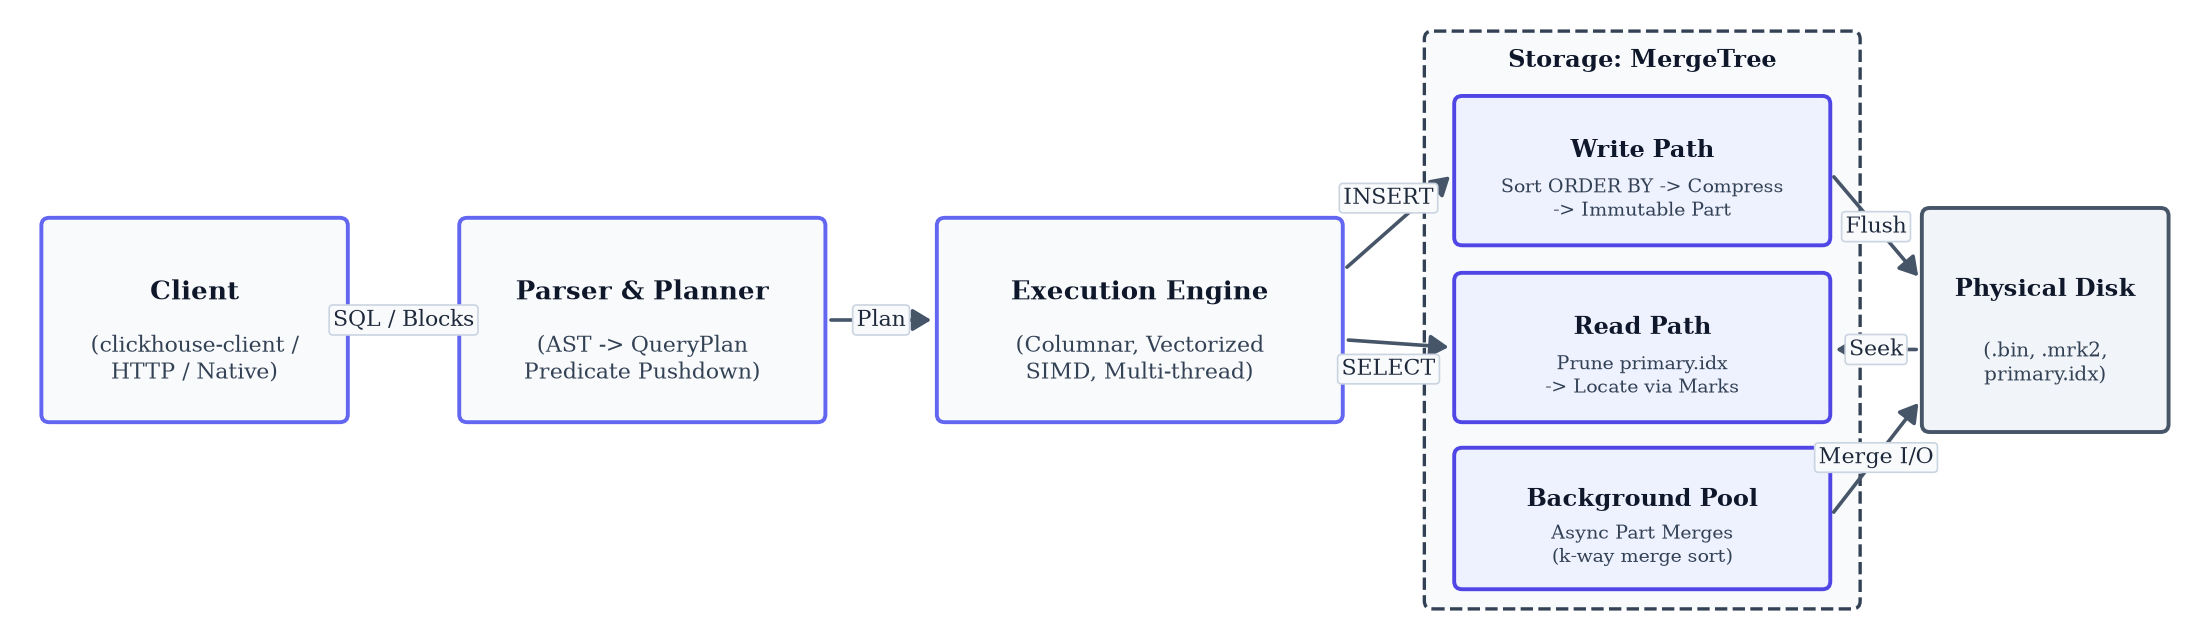
\includegraphics[width=0.95\textwidth,height=0.28\textheight,keepaspectratio]{fig2_1.png}
    }{
        \fbox{\parbox{0.9\textwidth}{\centering\vspace{0.5cm}\textbf{[Chèn Hình 2.1 -- tệp \texttt{fig2\_\allowbreak{}1.png}]}\vspace{0.5cm}}}
    }
    \caption{Luồng xử lý truy vấn tối thiểu trong ClickHouse và vị trí của động cơ MergeTree~\cite{A1, S2}.}
    \label{fig:fig2_1}
\end{figure}

\section{Data parts và đường ghi (Write Path) của MergeTree}
\subsection{Từ khối dữ liệu trong RAM đến phân đoạn bất biến}
Thay vì cập nhật trực tiếp tại chỗ vào trang đệm + WAL như B-tree, hay duy trì MemTable trên RAM như LSM-tree cổ điển, MergeTree xử lý từng lô \texttt{INSERT} qua 5~bước trong RAM rồi đóng thẳng thành thư mục phân đoạn bất biến (Hình~\ref{fig:fig2_2})~\cite{A1, S3, S9}:
\begin{enumerate}
    \setlength{\itemsep}{3pt}\setlength{\parskip}{0pt}
    \item \textbf{Phân khối (\textit{Block Parsing}):} Chuyển dòng byte đầu vào thành các khối mảng cột \texttt{Block} (giới hạn \texttt{max\_\allowbreak{}insert\_\allowbreak{}block\_\allowbreak{}size = 1.048.576}~dòng)~\cite{S9}.
    \item \textbf{Tách theo phân vùng (\textit{Partition Splitting}):} Chia thành các khối con sao cho mỗi khối chỉ chứa bản ghi thuộc duy nhất một giá trị \texttt{PARTITION BY}~\cite{S2, S3}.
    \item \textbf{Sắp xếp trong RAM theo \texttt{ORDER BY}:} Sắp xếp theo thứ tự từ điển trong từng khối con (MergeTree tiêu chuẩn không tự loại trùng các bản ghi cùng khóa)~\cite{S2}.
    \item \textbf{Cắt Granule, Nén cột \& Sinh chỉ mục:} Cắt dữ liệu thành hạt logic (mặc định 8.192~dòng), trích khóa dòng đầu mỗi hạt ghi vào \texttt{primary.idx}, nén từng cột vào khối nén ghi tệp \texttt{.bin} và ghi tọa độ vào tệp \textit{marks}~\cite{S3, S4}.
    \item \textbf{Công bố nguyên tử (\textit{Atomic Part Publication}):} Ghi ra thư mục tạm \texttt{tmp\_\allowbreak{}insert\_\allowbreak{}...} rồi đổi tên nguyên tử sang \texttt{<partition\_\allowbreak{}id>\_\allowbreak{}<min\_\allowbreak{}block>\_\allowbreak{}<max\_\allowbreak{}block>\_\allowbreak{}<level>} (ví dụ \texttt{201307\_\allowbreak{}1\_\allowbreak{}1\_\allowbreak{}0}) ở trạng thái \texttt{active = 1}~\cite{S3, S6}.
\end{enumerate}

Một lệnh \texttt{INSERT} đơn lẻ có thể tạo nhiều hơn 1~Data Part khi dữ liệu vượt cỡ khối \texttt{max\_\allowbreak{}insert\_\allowbreak{}block\_\allowbreak{}size}, trải rộng qua $k$~giá trị phân vùng khác nhau, hoặc chạy song song nhiều luồng chèn (\texttt{max\_\allowbreak{}insert\_\allowbreak{}threads > 1})~\cite{S3, S9}.

\begin{figure}[!htb]
    \centering
    \IfFileExists{fig2_2.png}{
        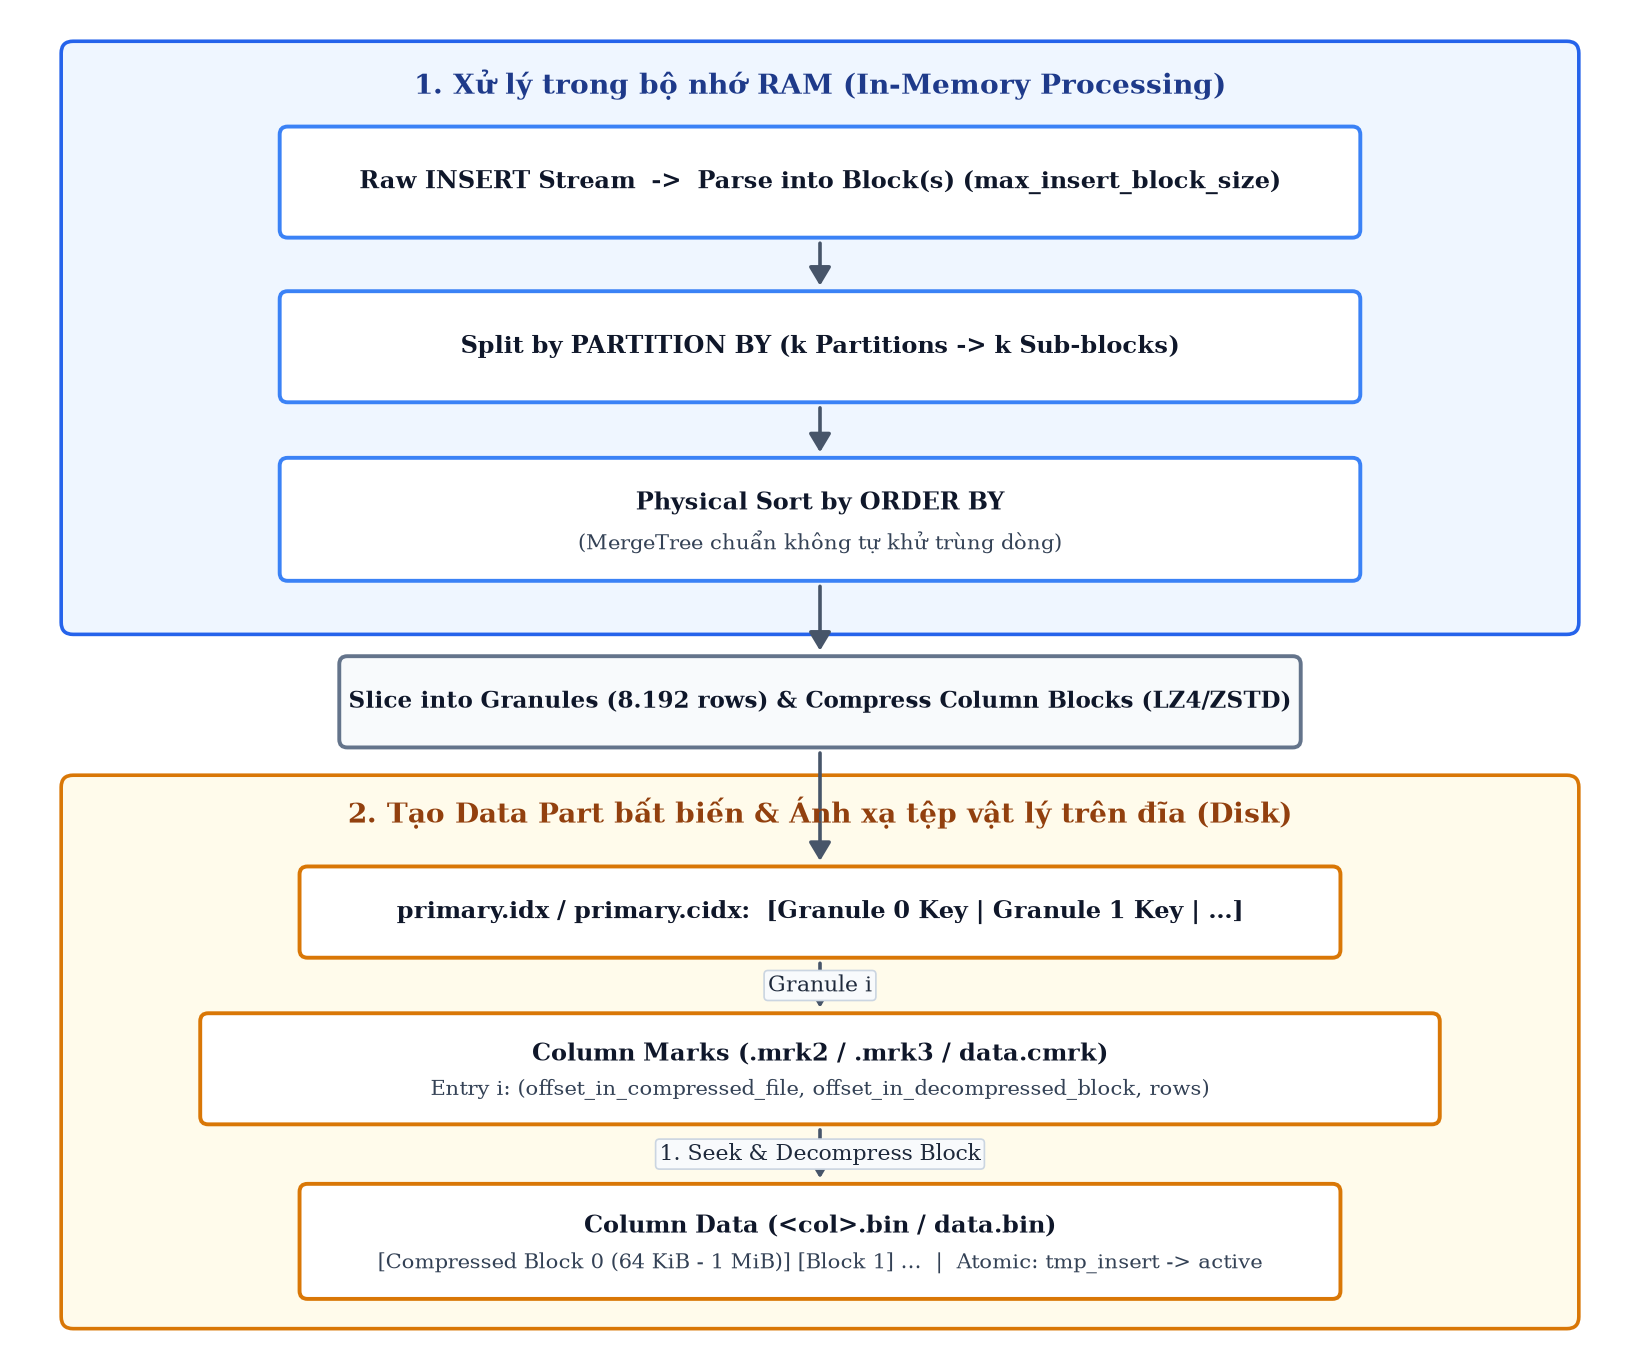
\includegraphics[width=0.88\textwidth,height=0.33\textheight,keepaspectratio]{fig2_2.png}
    }{
        \fbox{\parbox{0.9\textwidth}{\centering\vspace{0.5cm}\textbf{[Chèn Hình 2.2 -- tệp \texttt{fig2\_\allowbreak{}2.png}]}\vspace{0.5cm}}}
    }
    \caption{Đường ghi bất biến của MergeTree từ khối dữ liệu trong RAM đến tệp phân đoạn trên đĩa~\cite{A1, S3, S4}.}
    \label{fig:fig2_2}
\end{figure}

\subsection{Cấu trúc vật lý của Data Part: Wide/Compact, Khối nén và Marks}
Dựa trên ngưỡng \texttt{min\_\allowbreak{}bytes\_\allowbreak{}for\_\allowbreak{}wide\_\allowbreak{}part} (mặc định 10~MiB) và \texttt{min\_\allowbreak{}rows\_\allowbreak{}for\_\allowbreak{}wide\_\allowbreak{}part}, MergeTree tự động chọn: \textbf{Compact Part} gom tất cả các cột vào một tệp \texttt{data.bin} và \texttt{data.mrk3} để tiết kiệm inode hệ thống tệp cho các part nhỏ; \textbf{Wide Part} tách mỗi cột thành cặp tệp \texttt{<column>.bin} và \texttt{<column>.mrk2/\allowbreak{}.mrk3} độc lập để phục vụ quét cột chọn lọc tối ưu (Bảng~\ref{tab:data_part_files})~\cite{S3, S4}.

\begin{table}[!htb]
\centering
\footnotesize
\renewcommand{\arraystretch}{1.14}
\caption{Cấu trúc tệp tiêu biểu trong thư mục Data Part (định dạng Wide)}
\label{tab:data_part_files}
\begin{tabularx}{\textwidth}{>{\ttfamily\raggedright\arraybackslash}p{4.35cm} >{\raggedright\arraybackslash}X}
\toprule
\textrm{\textbf{Tên tệp vật lý}} & \textbf{Vai trò trong kiến trúc lưu trữ và truy xuất} \\
\midrule
<column>.bin & Dữ liệu cột chia thành các Compressed Block liên tiếp (mặc định LZ4, 64~KiB--1~MiB chưa nén)~\cite{S3}. \\
\addlinespace[3pt]
<column>.mrk2 / .mrk3 / .cmrk2 & Tệp đánh dấu (\textit{Marks}) nối Granule logic với bộ tọa độ 2~tầng trong \texttt{.bin}~\cite{S4}. \\
\addlinespace[3pt]
primary.idx / primary.cidx & Chỉ mục chính thưa lưu giá trị \texttt{PRIMARY KEY} của dòng đầu tiên mỗi Granule~\cite{S4}. \\
\addlinespace[3pt]
count.txt / columns.txt & Tổng số hàng trong part (phục vụ \texttt{count()} tức thì) và lược đồ kiểu dữ liệu của part~\cite{S3}. \\
\addlinespace[3pt]
checksums.txt / minmax\_<col>.idx & Tổng kiểm tra toàn vẹn mọi tệp và cặp min/max cột phân vùng phục vụ cắt tỉa phân vùng~\cite{S2, S3}. \\
\bottomrule
\end{tabularx}
\end{table}

Cần phân biệt rạch ròi giữa \textbf{Granule} (đơn vị đọc/lọc logic nhỏ nhất, mặc định 8.192~dòng) và \textbf{Compressed Block} (khối nén vật lý trong \texttt{.bin} gom từ 64~KiB đến 1~MiB dữ liệu chưa nén tùy kiểu cột)~\cite{A1, S4}. Vì độ dài khối nén thay đổi theo độ nén thực tế, ClickHouse không thể định vị Granule thứ~$k$ bằng phép nhân trực tiếp mà dùng bộ ba thông tin trong tệp Marks: \texttt{offset\_\allowbreak{}in\_\allowbreak{}compressed\_\allowbreak{}file} (vị trí khối nén trong \texttt{.bin}), \texttt{offset\_\allowbreak{}in\_\allowbreak{}decompressed\_\allowbreak{}block} (vị trí bắt đầu hạt trong vùng nhớ RAM sau khi giải nén) và \texttt{rows\_\allowbreak{}num}. Khi truy xuất, hệ thống gọi \texttt{lseek} nhảy thẳng tới khối nén tương ứng trên đĩa, giải nén duy nhất khối 64~KiB--1~MiB đó vào RAM rồi dịch tới đúng \textit{offset} bên trong khối.

\subsection{Phân cấp Table -- Partition -- Part -- Granule và Minh họa lược đồ}
MergeTree tổ chức dữ liệu theo 4~cấp phân cấp (Hình~\ref{fig:fig2_3})~\cite{S2, S3}: \textbf{Table} $\rightarrow$ \textbf{Partition} (nhóm theo \texttt{PARTITION BY}) $\rightarrow$ \textbf{Data Part} bất biến lưu dưới cây thư mục \texttt{store/\allowbreak{}<table\_\allowbreak{}uuid>/\allowbreak{}<part\_\allowbreak{}name>/\allowbreak{}} $\rightarrow$ \textbf{Granule}. Một quy tắc bất biến sống còn là \textit{các Data Part thuộc hai Partition khác nhau không bao giờ được hợp nhất với nhau}~\cite{S3, S5}. Do đó, \texttt{PARTITION BY} chỉ nên dùng quản trị vòng đời (DROP/TTL) và cắt tỉa phân vùng thô; chọn khóa phân vùng quá chi li (như theo \texttt{UserID} hoặc từng phút) sẽ xé lẻ bảng thành hàng trăm phân vùng không thể gộp, trực tiếp kích hoạt lỗi \textit{Too many parts}~\cite{S2, S9}. Vì tập dữ liệu ClickBench đều nằm trọn trong tháng 07/2013 (\texttt{201307})~\cite{B5}, lược đồ thực nghiệm Chương~3--4 bỏ qua phân vùng (mặc định 1~partition \texttt{tuple()}) để cô lập thuần túy tác động của \texttt{ORDER BY} và \texttt{index\_\allowbreak{}granularity}~\cite{M6}.

\begin{figure}[!htb]
    \centering
    \IfFileExists{fig2_3.png}{
        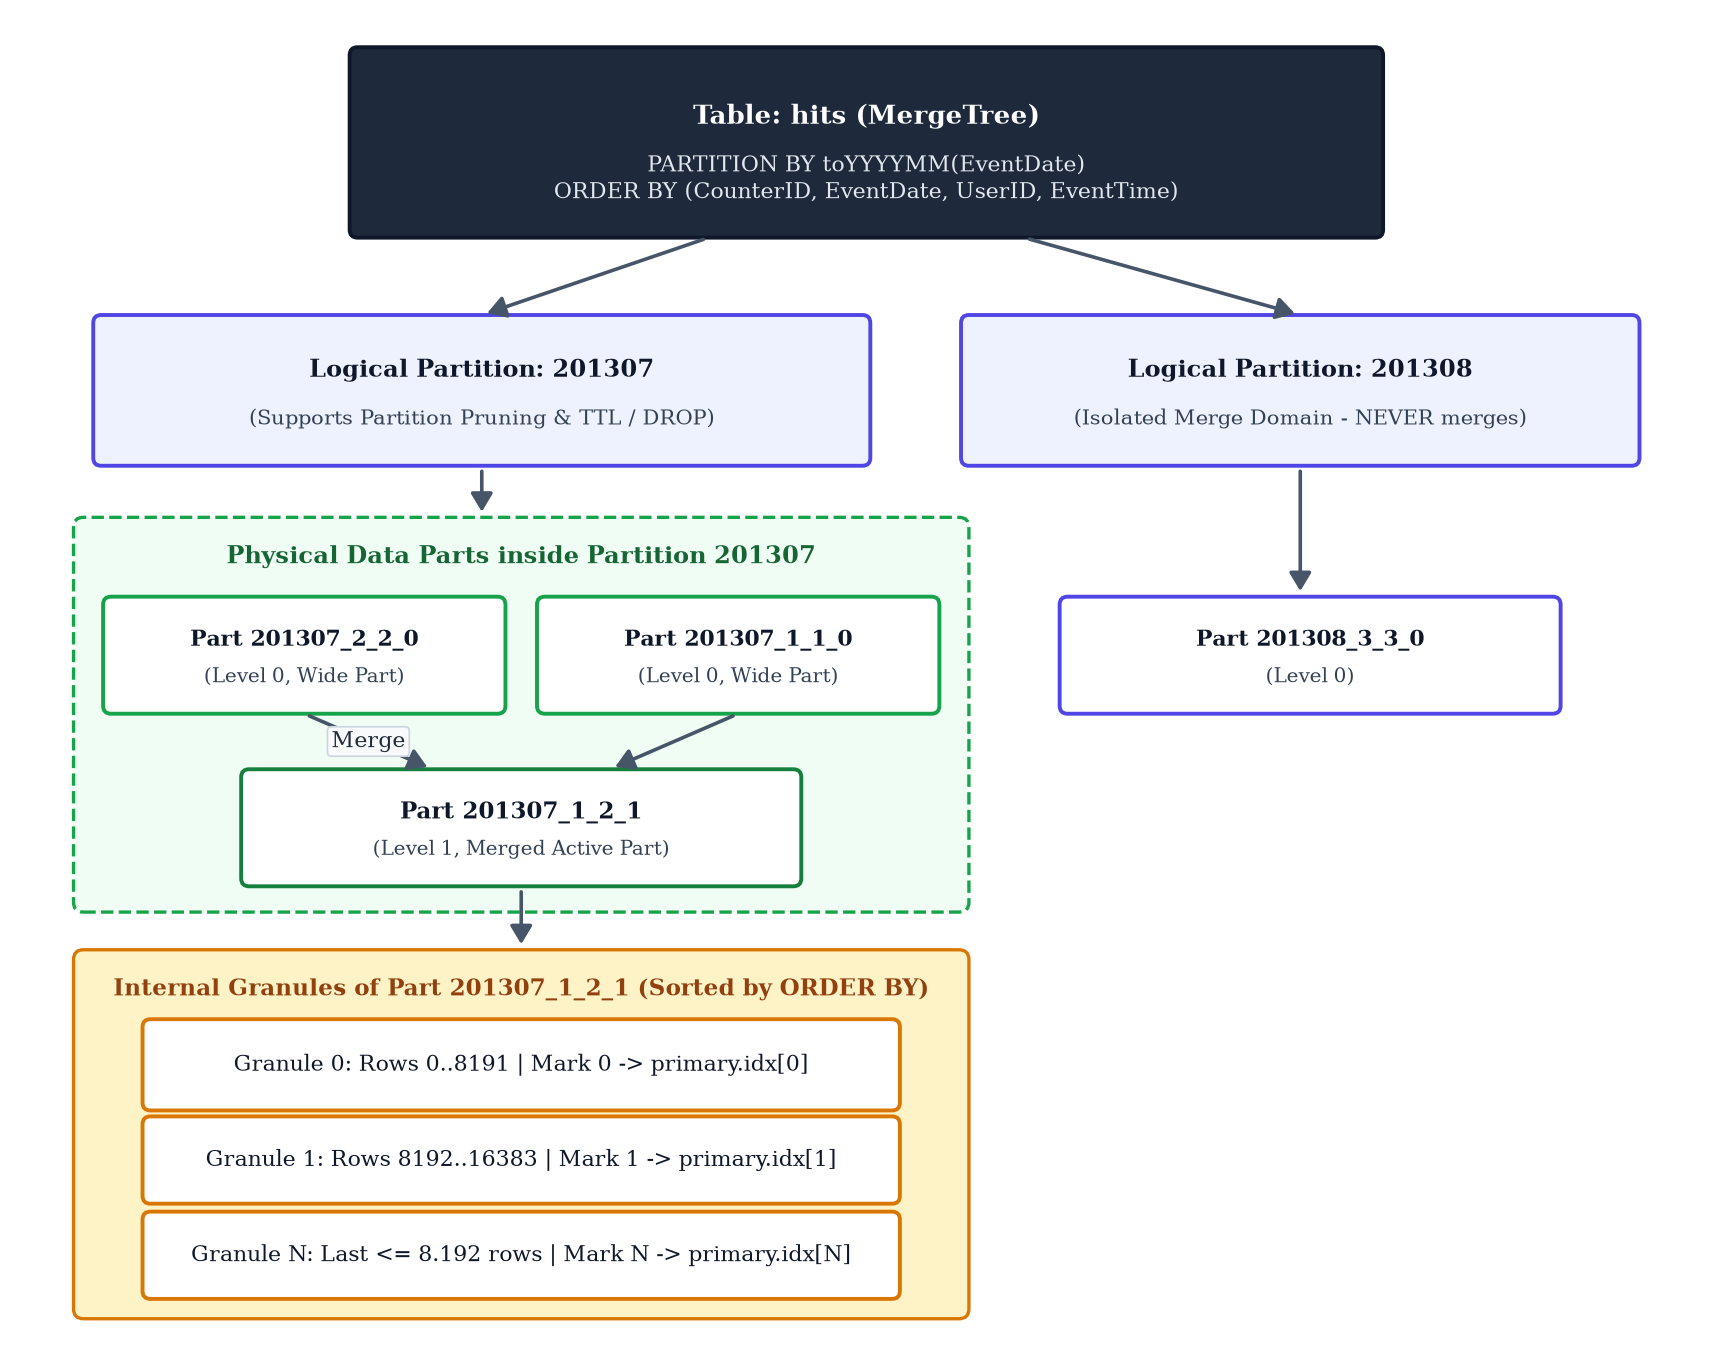
\includegraphics[width=0.88\textwidth,height=0.33\textheight,keepaspectratio]{fig2_3.png}
    }{
        \fbox{\parbox{0.9\textwidth}{\centering\vspace{0.5cm}\textbf{[Chèn Hình 2.3 -- tệp \texttt{fig2\_\allowbreak{}3.png}]}\vspace{0.5cm}}}
    }
    \caption{Quan hệ phân cấp giữa Table, Partition, Data Part và Granule trong động cơ MergeTree~\cite{S2, S3}.}
    \label{fig:fig2_3}
\end{figure}

\begin{tcolorbox}[sqlblock]
\setlength{\topsep}{0pt}\setlength{\partopsep}{0pt}\footnotesize\setstretch{1.05}
\begin{verbatim}
-- Lược đồ ClickBench gốc (105 cột [B5]) & kiểm tra system.parts [S6]
CREATE TABLE default.hits (
    WatchID BIGINT, EventTime TIMESTAMP, EventDate Date,
    CounterID INTEGER, RegionID INTEGER, UserID BIGINT, ...
) ENGINE = MergeTree()
PARTITION BY toYYYYMM(EventDate)
PRIMARY KEY (CounterID, EventDate, intHash32(UserID))
ORDER BY (CounterID, EventDate, intHash32(UserID), EventTime)
SETTINGS index_granularity = 8192;

SELECT partition, name AS part_name, part_type, active, marks, rows,
       formatReadableSize(bytes_on_disk) AS size_on_disk
FROM system.parts
WHERE database = 'default' AND table = 'hits' AND active = 1
ORDER BY name ASC;
\end{verbatim}
\end{tcolorbox}

\section{Khóa sắp xếp (\texorpdfstring{\texttt{ORDER BY}}{ORDER BY}), Khóa chính và Chỉ mục chính thưa}
\needspace{4\baselineskip}
\noindent\textbf{Phân biệt \texttt{ORDER BY}, \texttt{PRIMARY KEY} và Thuật toán duyệt chỉ mục:}
\texttt{ORDER BY} xác định thứ tự sắp xếp vật lý các dòng trong từng Data Part và thứ tự trộn khi hợp nhất nền, còn \texttt{PRIMARY KEY} (mặc định bằng \texttt{ORDER BY}, hoặc có thể là tiền tố ngắn hơn) quy định bộ khóa được trích tại dòng đầu mỗi granule lưu trong \texttt{primary.idx} nạp thường trực trên RAM~\cite{S2, S4}. Khác hoàn toàn với RDBMS, khóa chính trong MergeTree \textit{không ép ràng buộc duy nhất}: nhiều bản ghi trùng khóa vẫn cùng tồn tại liền kề nhau. Thực nghiệm E1 đối chứng 3~biến thể khóa: $K_0 = \texttt{tuple()}$, $K_1 = \texttt{(\allowbreak{}CounterID, EventDate)}$ và $K_2 = \texttt{(\allowbreak{}EventDate, CounterID)}$.

Hình~\ref{fig:fig2_4} minh họa phân bố hạt thỏa điều kiện lọc trên 16~bản ghi giả định ($g = 4$). Do chỉ mục thưa chỉ lưu mốc dòng đầu mỗi hạt, một hạt ở vùng biên có thể bị chọn đọc kể cả khi phần khớp nằm ở đầu hạt kế tiếp. Dựa trên cấu trúc khóa, ClickHouse kích hoạt 2~giải thuật duyệt chỉ mục~\cite{S4a} (Bảng~\ref{tab:prefix_utilization}):
\begin{itemize}
    \setlength{\itemsep}{3pt}\setlength{\parskip}{0pt}
    \item \textbf{Tìm kiếm nhị phân (\textit{Binary Search}, $O(\log_2 M)$):} Kích hoạt khi câu truy vấn lọc trực tiếp trên cột đứng đầu khóa (W1 với $K_1$, W2 với $K_2$), khoanh vùng dải đọc về đúng 1~dải liên tục.
    \item \textbf{Loại trừ tổng quát (\textit{Generic Exclusion Search}):} Kích hoạt khi khuyết cột tiền tố mà chỉ lọc cột phía sau (W1 trên $K_2$ hoặc W2 trên $K_1$). Hệ thống duyệt từng khoảng mốc $[K_i, K_{i+1}]$ trong RAM để loại hạt không giao cắt; hiệu quả vẫn tốt nếu cột đứng trước có lực lượng phân biệt nhỏ (như 17~ngày), nhưng trở nên vô hiệu nếu tiền tố quá phân tán~\cite{S4, S4a}.
\end{itemize}

\begin{figure}[!htb]
    \centering
    \IfFileExists{fig2_4.png}{
        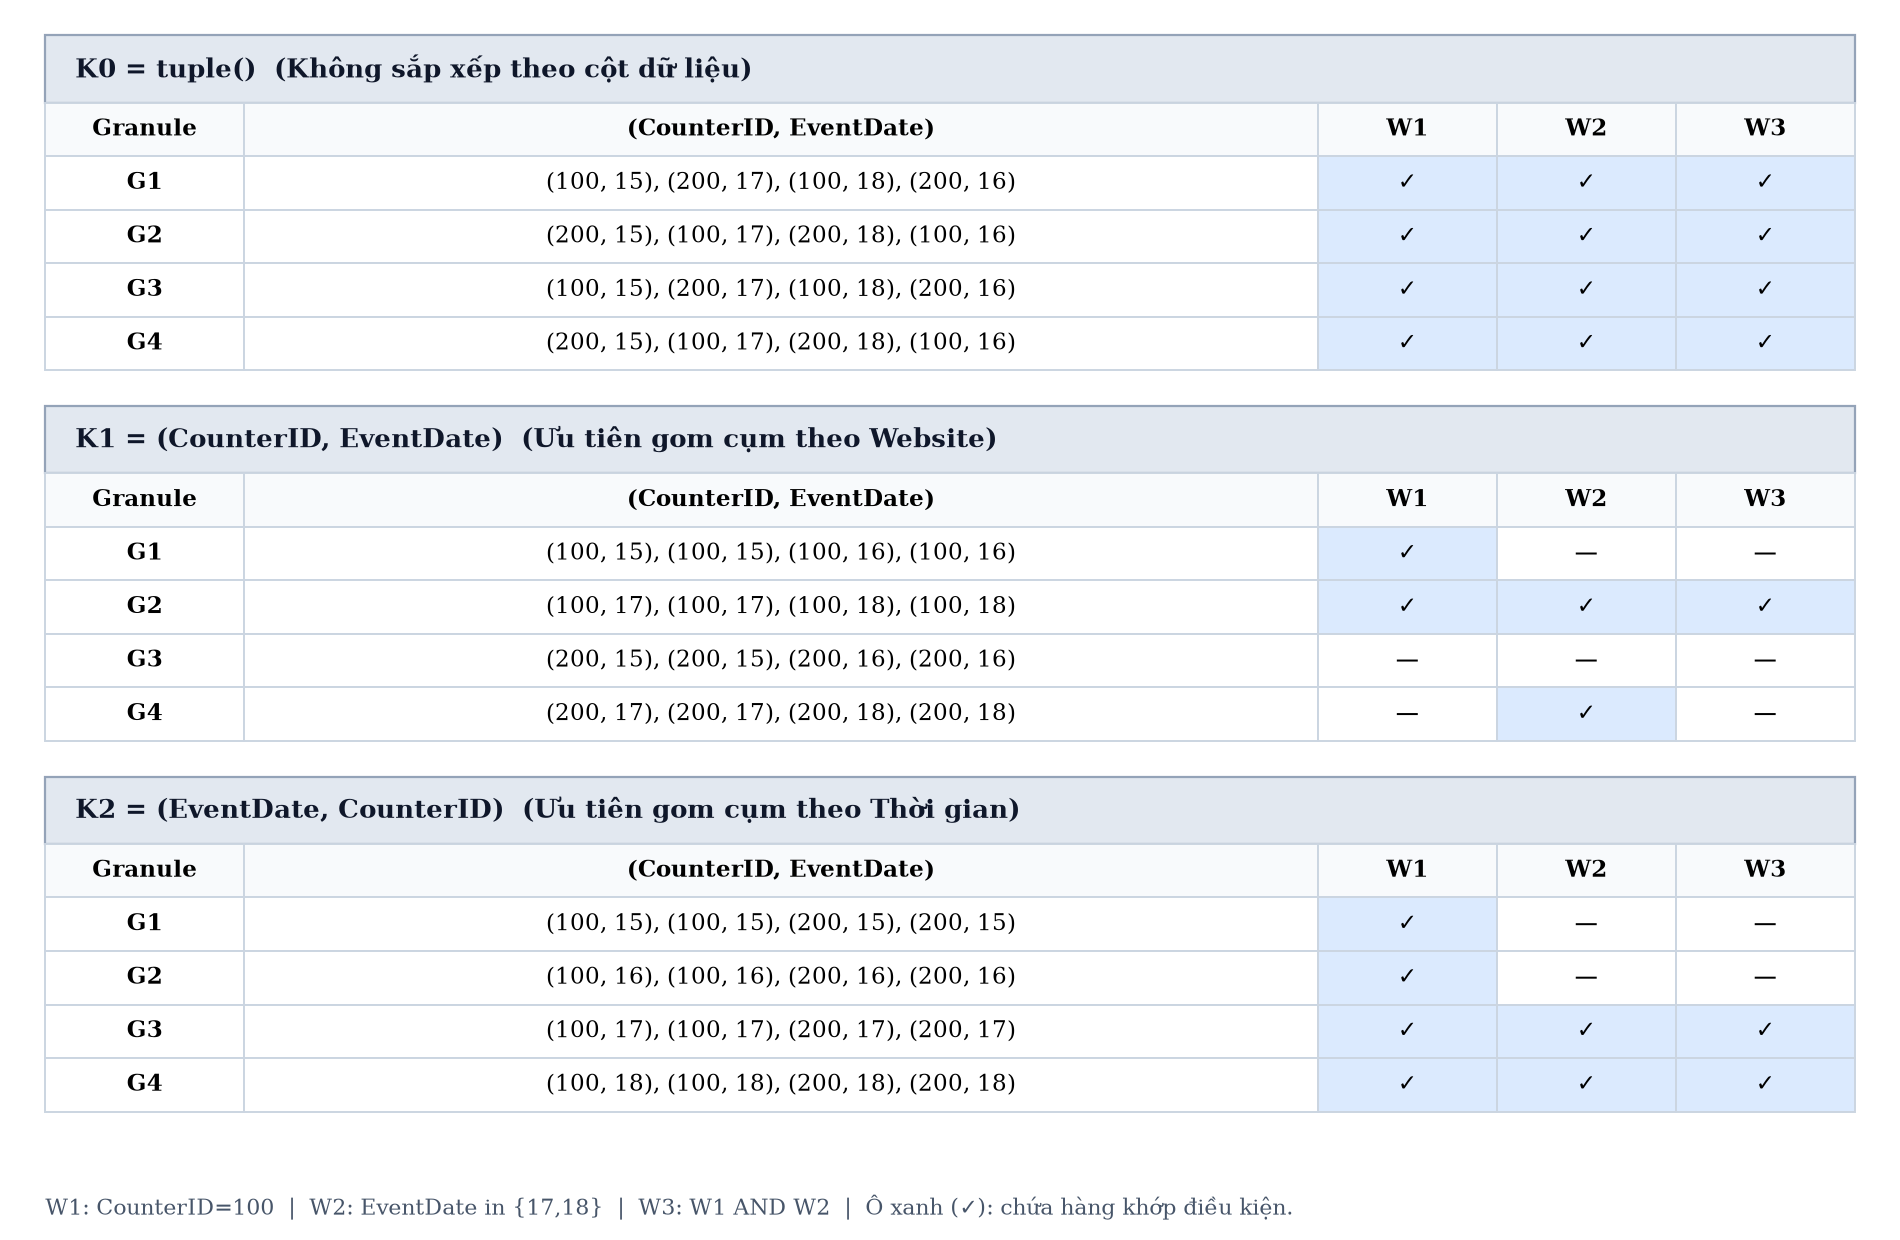
\includegraphics[width=0.88\textwidth,height=0.29\textheight,keepaspectratio]{fig2_4.png}
    }{
        \fbox{\parbox{0.9\textwidth}{\centering\vspace{0.5cm}\textbf{[Chèn Hình 2.4 -- tệp \texttt{fig2\_\allowbreak{}4.png}]}\vspace{0.5cm}}}
    }
    \caption{Phân bố granule chứa hàng khớp bộ lọc với $K_0$, $K_1$ và $K_2$ trên 16~bản ghi giả định; dấu~$\checkmark$ không phải kết quả chọn marks của ClickHouse. Nguồn: Nhóm xây dựng theo~\cite{S2, S4}.}
    \label{fig:fig2_4}
\end{figure}

\begin{table}[!htb]
\centering
\footnotesize
\renewcommand{\arraystretch}{1.14}
\caption{Khả năng tận dụng tiền tố khóa theo nhóm bộ lọc khảo sát (đánh giá định tính theo~\cite{S4, S4a})}
\label{tab:prefix_utilization}
\begin{tabularx}{\textwidth}{>{\bfseries\raggedright\arraybackslash}p{2.9cm} >{\raggedright\arraybackslash}X >{\raggedright\arraybackslash}X >{\raggedright\arraybackslash}p{3.6cm}}
\toprule
\textbf{Bộ lọc} & \textbf{$K_1$:} \texttt{(\allowbreak{}CounterID, EventDate)} & \textbf{$K_2$:} \texttt{(\allowbreak{}EventDate, CounterID)} & \textbf{Nội dung kiểm chứng} \\
\midrule
W1: \texttt{CounterID} & Có tiền tố (Binary Search) & Không tiền tố (Generic Exclusion) & Granules (\texttt{EXPLAIN}), latency \\
\addlinespace[3pt]
W2: \texttt{EventDate} & Không tiền tố (Generic Exclusion) & Có tiền tố (Binary Search) & Granules (\texttt{EXPLAIN}), latency \\
\addlinespace[3pt]
W3: kết hợp & Tiền tố \texttt{CounterID} & Tiền tố \texttt{EventDate} & Granules, độ trễ \& nén \\
\addlinespace[3pt]
W4: \texttt{RegionID} & Không thuộc khóa & Không thuộc khóa & Toàn bảng (0\% pruning) \\
\bottomrule
\end{tabularx}
\end{table}

\section{Granules, Marks và Quá trình đọc có chọn lọc}
\needspace{4\baselineskip}
\noindent\textbf{\texttt{index\_\allowbreak{}granularity}, Kiểm chứng \texttt{EXPLAIN} và Mô hình giải tích:}
Tham số \texttt{index\_\allowbreak{}granularity} (mặc định 8.192~dòng) xác định độ mịn hạt dữ liệu; kết hợp giới hạn byte thích ứng \texttt{index\_\allowbreak{}granularity\_\allowbreak{}bytes} (mặc định 10~MiB). Đối với lược đồ hẹp 12~cột số nguyên dài 44~byte/dòng tại Chương~3, một hạt 8.192~dòng chỉ chiếm $8.192 \times 44~\text{B} \approx 360~\text{KiB} \ll 10~\text{MiB}$, chứng minh việc cố định \texttt{index\_\allowbreak{}granularity\_\allowbreak{}bytes = 0} ở Thực nghiệm~E2 hoàn toàn giữ nguyên hành vi phân hạt mặc định trên thực tế để cô lập $g \in \{2.048;\, 8.192;\, 32.768\}$~\cite{S2} (trái lại, ở \textbf{Chương~5} khi cột trạng thái HLL nặng $\approx 2{,}59~\text{KiB/dòng}$, tức 2.651~B, ngưỡng 10~MiB sẽ tự kích hoạt).

Xét 1~active part gồm $N$~hàng với độ mịn $g$: tổng số marks là $M \approx \lceil N/g \rceil$, lượng dòng ước lượng đọc khi chọn $k$~granules là $R_{\text{est}} \approx \min(N, k \times g)$, và kích thước phần khóa trong RAM là $I_{\text{key}} \approx M \times s_{\text{key}}$ (Hình~\ref{fig:fig2_5})~\cite{S2, S4}. Với $N = 30.000.000$, $g = 8.192$ và độ rộng khóa $K_1$ là $s_{\text{key}} = 4 + 2 = 6~\text{B}$: ta có $M = 3.663$~marks và $I_{\text{key}} = 3.663 \times 6 = 21.978~\text{B}$ ($\approx 21{,}5~\text{KiB}$, chưa tính overhead tệp marks). Hạ $g$ giảm lượng hàng đọc thừa nhưng làm phình danh sách marks và tăng chi phí điều phối từng khối nén; hai lệnh \texttt{EXPLAIN indexes = 1}, \texttt{EXPLAIN ESTIMATE} cùng \texttt{system.\allowbreak{}parts} dùng để đối chứng kế hoạch cắt tỉa trước khi đối chiếu với \texttt{read\_\allowbreak{}rows} thực tế từ \texttt{system.\allowbreak{}query\_\allowbreak{}log} (tắt \texttt{PREWHERE} và cache trong E1/E2)~\cite{S6, S7, S10}:

\begin{figure}[!htb]
    \centering
    \IfFileExists{fig2_5.png}{
        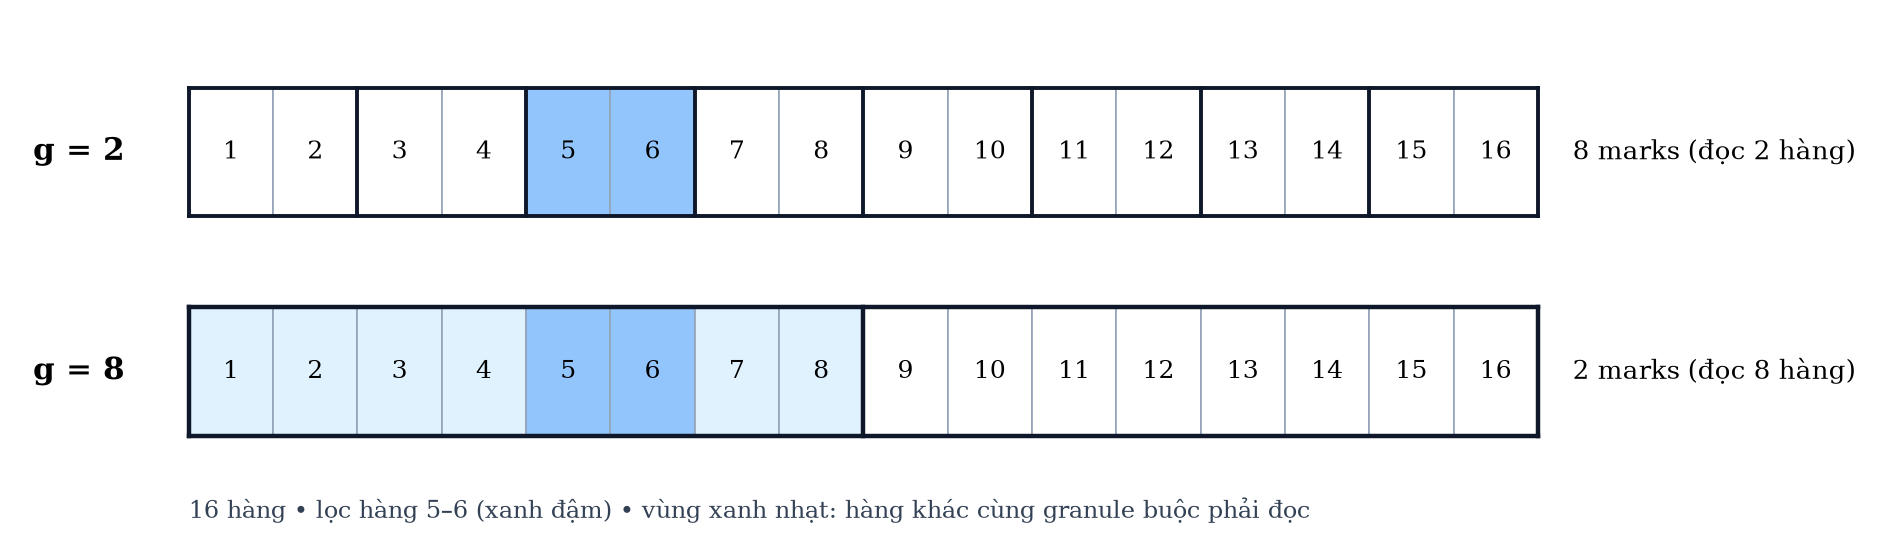
\includegraphics[width=0.88\textwidth,height=0.27\textheight,keepaspectratio]{fig2_5.png}
    }{
        \fbox{\parbox{0.9\textwidth}{\centering\vspace{0.5cm}\textbf{[Chèn Hình 2.5 -- tệp \texttt{fig2\_\allowbreak{}5.png}]}\vspace{0.5cm}}}
    }
    \caption{So sánh granule nhỏ/lớn trên 16~hàng giả định: xanh đậm là hàng 5--6 thỏa lọc, xanh nhạt là các hàng khác cùng granule phải đọc. Nguồn: Nhóm xây dựng theo~\cite{S2, S4}.}
    \label{fig:fig2_5}
\end{figure}

\begin{tcolorbox}[sqlblock]
\setlength{\topsep}{0pt}\setlength{\partopsep}{0pt}\footnotesize\setstretch{1.05}
\begin{verbatim}
EXPLAIN indexes = 1 -- hoặc EXPLAIN ESTIMATE (đọc marks/rows dự kiến)
SELECT count(), sum(ResolutionWidth) FROM hits_k1
WHERE CounterID = 3258
  AND EventDate >= toDate('2013-07-15')
  AND EventDate < toDate('2013-07-23')
SETTINGS use_query_condition_cache = 0, use_skip_indexes_on_data_read = 0;

SELECT name, rows, marks, marks_bytes, primary_key_bytes_in_memory
FROM system.parts WHERE active = 1 AND table = 'hits_k1' ORDER BY name;
\end{verbatim}
\end{tcolorbox}

\section{Tiến trình Hợp nhất nền (Background Merges) và Hệ biến thể}
\subsection{Cơ chế k-way merge sort, Kích thước lô và Quan sát qua system tables}
Tiến trình \textit{background merge} đọc các phân đoạn cùng partition, chạy thuật toán \textit{k-way merge sort} theo \texttt{ORDER BY}, dựng lại \texttt{primary.idx}/\textit{marks} rồi công bố part mới ở trạng thái \texttt{active = 1} trước khi chuyển các part nguồn sang \texttt{inactive} (Hình~\ref{fig:fig2_6})~\cite{S3, S5, S6}. Với tổng $N$~dòng nạp theo lô kích thước $B$, client phát $\lceil N/B \rceil$ yêu cầu \texttt{INSERT} (Hình~\ref{fig:fig2_7})~\cite{S9}: lô nhỏ tạo nhiều part rời rạc, đội chi phí \texttt{fsync}/giao thức và dễ chạm trần \textit{Too many parts}, còn lô lớn giảm áp lực hợp nhất nhưng tăng bộ nhớ đệm và trễ gom lô đầu phát~\cite{S9, S13}. ClickHouse khuyến cáo tránh lạm dụng \texttt{OPTIMIZE TABLE ... FINAL} trong luồng nạp thực tế vì ép merge nặng toàn phần; thay vào đó E3 giữ merge nền tự nhiên~\cite{S12}. Thời lượng $T_{\text{ACK}}$ tách biệt hoàn toàn khỏi tổng thời gian merge song song ($\Sigma\text{duration\_ms}$) và hệ số đọc lặp gộp $\Sigma r / N$ trích từ \texttt{system.\allowbreak{}part\_\allowbreak{}log} (Bảng~\ref{tab:e3_metrics})~\cite{S6, S8, S11}.

\begin{figure}[!htb]
    \centering
    \IfFileExists{fig2_6.png}{
        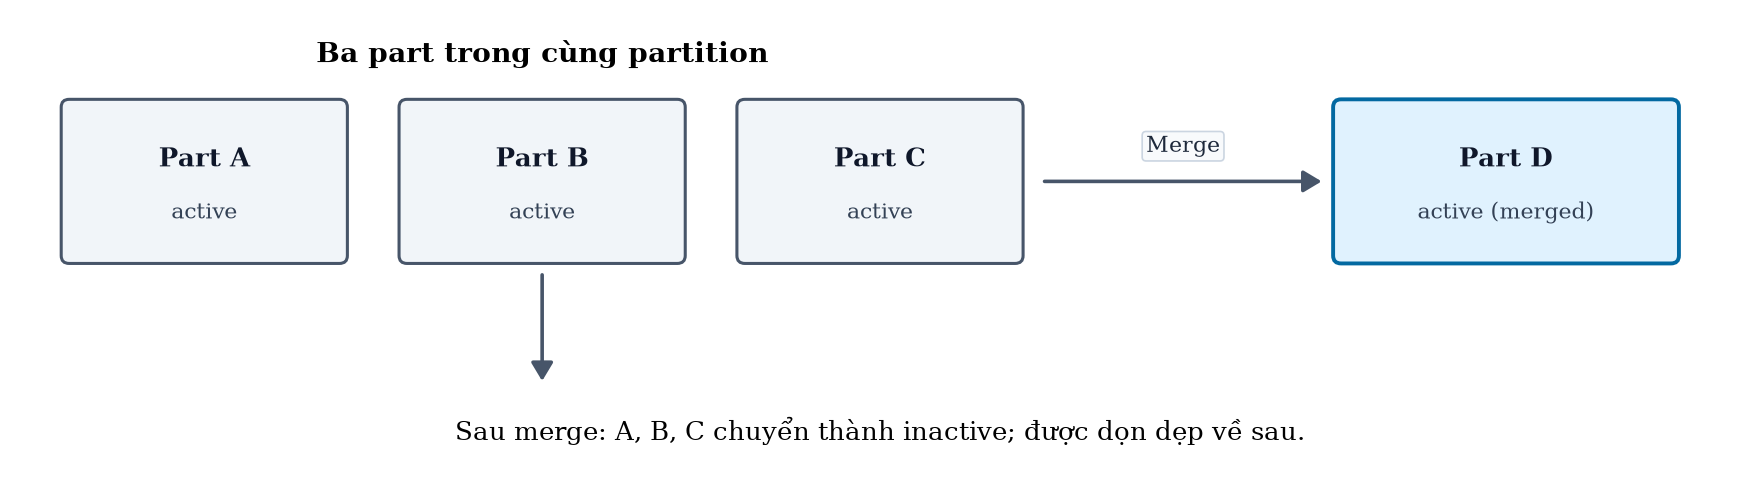
\includegraphics[width=0.84\textwidth,height=0.26\textheight,keepaspectratio]{fig2_6.png}
    }{
        \fbox{\parbox{0.9\textwidth}{\centering\vspace{0.5cm}\textbf{[Chèn Hình 2.6 -- tệp \texttt{fig2\_\allowbreak{}6.png}]}\vspace{0.5cm}}}
    }
    \caption{Minh họa do nhóm vẽ: A, B, C cùng partition được hợp nhất thành D. Sơ đồ không phải số đo thực nghiệm; cơ chế theo~\cite{S3, S5}.}
    \label{fig:fig2_6}
\end{figure}

\begin{figure}[!htb]
    \centering
    \IfFileExists{fig2_7.png}{
        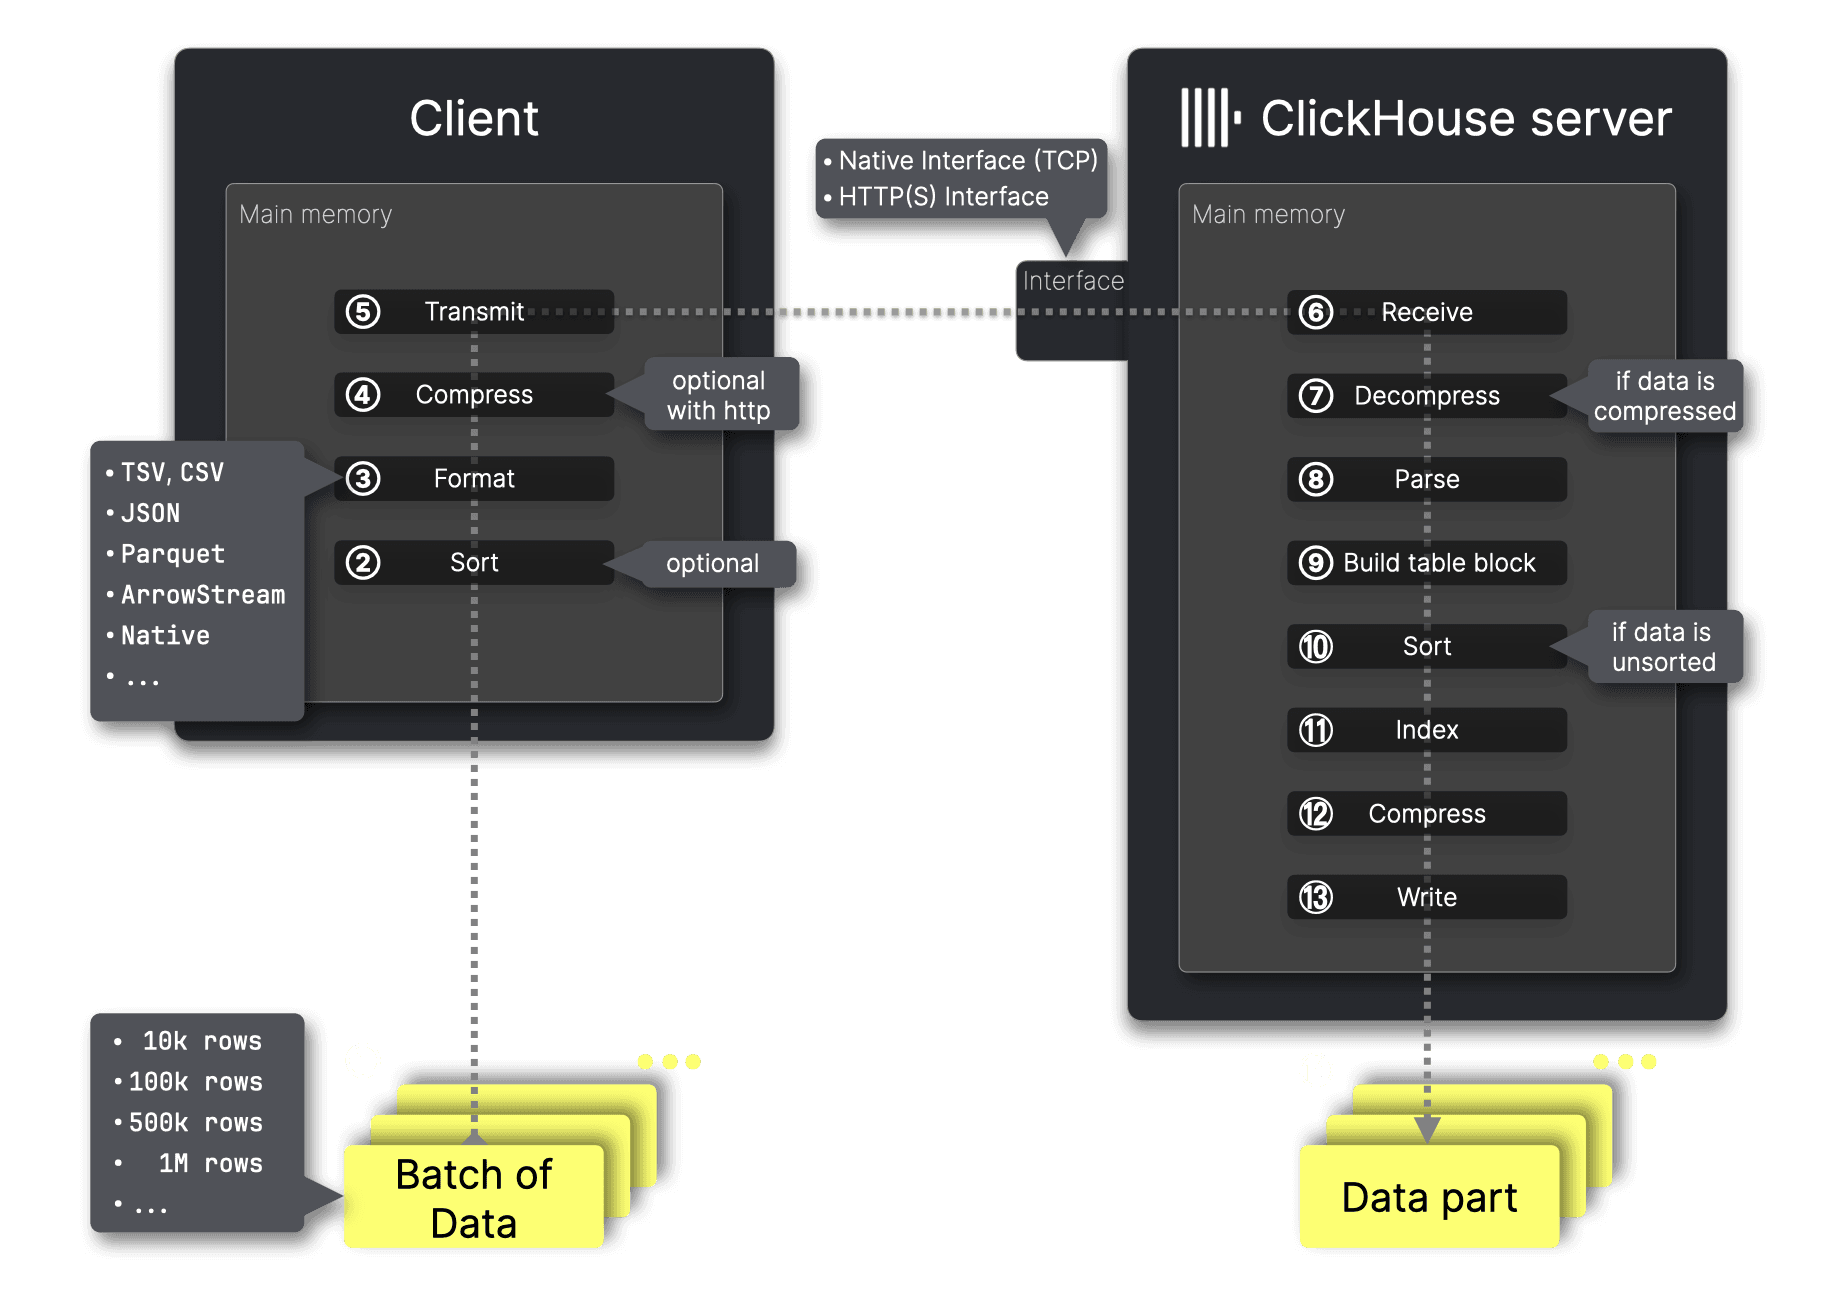
\includegraphics[width=0.86\textwidth,height=0.32\textheight,keepaspectratio]{fig2_7.png}
    }{
        \fbox{\parbox{0.9\textwidth}{\centering\vspace{0.5cm}\textbf{[Chèn Hình 2.7 -- tệp \texttt{fig2\_\allowbreak{}7.png}]}\vspace{0.5cm}}}
    }
    \caption{Các bước xử lý một yêu cầu \texttt{INSERT} đồng bộ để tạo data part. Nguồn: ClickHouse Docs, ``Selecting an insert strategy''~\cite{S9} $\cdot$ CC BY-NC-SA~4.0.}
    \label{fig:fig2_7}
\end{figure}

\begin{table}[!htb]
\centering
\footnotesize
\renewcommand{\arraystretch}{1.14}
\caption[Đại lượng đo lường phục vụ E3 và nguồn lấy]{Đại lượng phục vụ E3 và nguồn lấy ($N$: số dòng đầu vào đã kiểm tra; $r$: \texttt{read\_rows} của một sự kiện \texttt{MergeParts} thành công)}
\label{tab:e3_metrics}
\begin{tabularx}{\textwidth}{>{\raggedright\arraybackslash}p{4.1cm} >{\raggedright\arraybackslash}p{3.9cm} >{\raggedright\arraybackslash}X}
\toprule
\textbf{Đại lượng} & \textbf{Nguồn lấy} & \textbf{Ý nghĩa và giới hạn} \\
\midrule
$T_{\text{ACK}}$~(s); $N/T_{\text{ACK}}$~(dòng/s) & Đồng hồ chương trình nạp & Thời gian nhận phản hồi; tốc độ nạp. Không đo chờ gom lô. \\
\addlinespace[3pt]
Số active part; $\Sigma$\,\texttt{bytes\_\allowbreak{}on\_\allowbreak{}disk} & \texttt{system.\allowbreak{}parts}, \texttt{active=1} & Trạng thái thời điểm lấy mẫu; chưa phải đỉnh dung lượng đĩa. \\
\addlinespace[3pt]
Merge chạy / lịch sử ($\Sigma\text{dur}$, $\Sigma r$) & \texttt{system.\allowbreak{}merges}; \texttt{part\_\allowbreak{}log} & Lưu ý các merge chạy song song nên $\Sigma\text{dur}$ không cộng vào $T_{\text{ACK}}$. \\
\addlinespace[3pt]
$\Sigma r / N$; chờ ổn định~(s) & Dẫn xuất từ log/đồng hồ & Hệ số đọc lặp gộp ở mức logic (không phải byte ghi SSD vật lý). \\
\bottomrule
\end{tabularx}
\end{table}

\FloatBarrier
\subsection{Phạm vi áp dụng họ động cơ MergeTree}
Tận dụng ngay pha hợp nhất nền, ClickHouse mở rộng \texttt{MergeTree} chuẩn thành 4~biến thể chuyên biệt:
\begin{itemize}
    \setlength{\itemsep}{3pt}\setlength{\parskip}{0pt}
    \item \textbf{\texttt{ReplacingMergeTree(ver)} (Hình~\ref{fig:fig2_8}):} Giữ một bản ghi theo khóa \texttt{ORDER BY} (ưu tiên cột \texttt{ver} lớn nhất) khi merge nền chạy; cần \texttt{SELECT ... FINAL} hoặc bộ lọc cấp ứng dụng nếu yêu cầu khử trùng tức thời trước khi merge xong (dùng ở \textbf{Chương~5} cho bảng đối soát \texttt{event\_\allowbreak{}id})~\cite{V1}.
    \item \textbf{\texttt{SummingMergeTree}:} Tự động cộng dồn các cột số cùng khóa khi hợp nhất part~\cite{V2}.
    \item \textbf{\texttt{AggregatingMergeTree}:} Hợp nhất trạng thái nhị phân của các hàm tổng hợp phi tuyến qua cặp hàm \texttt{-State} và \texttt{-Merge} (nền tảng chính của bài toán \textbf{Chương~5})~\cite{V3}.
    \item \textbf{\texttt{ReplicatedMergeTree}:} Duy trì bản sao đa máy chủ thông qua ClickHouse Keeper theo cơ chế nhân bản bất đồng bộ mặc định~\cite{V4}.
\end{itemize}

\begin{figure}[!htb]
    \centering
    \IfFileExists{fig2_8.png}{
        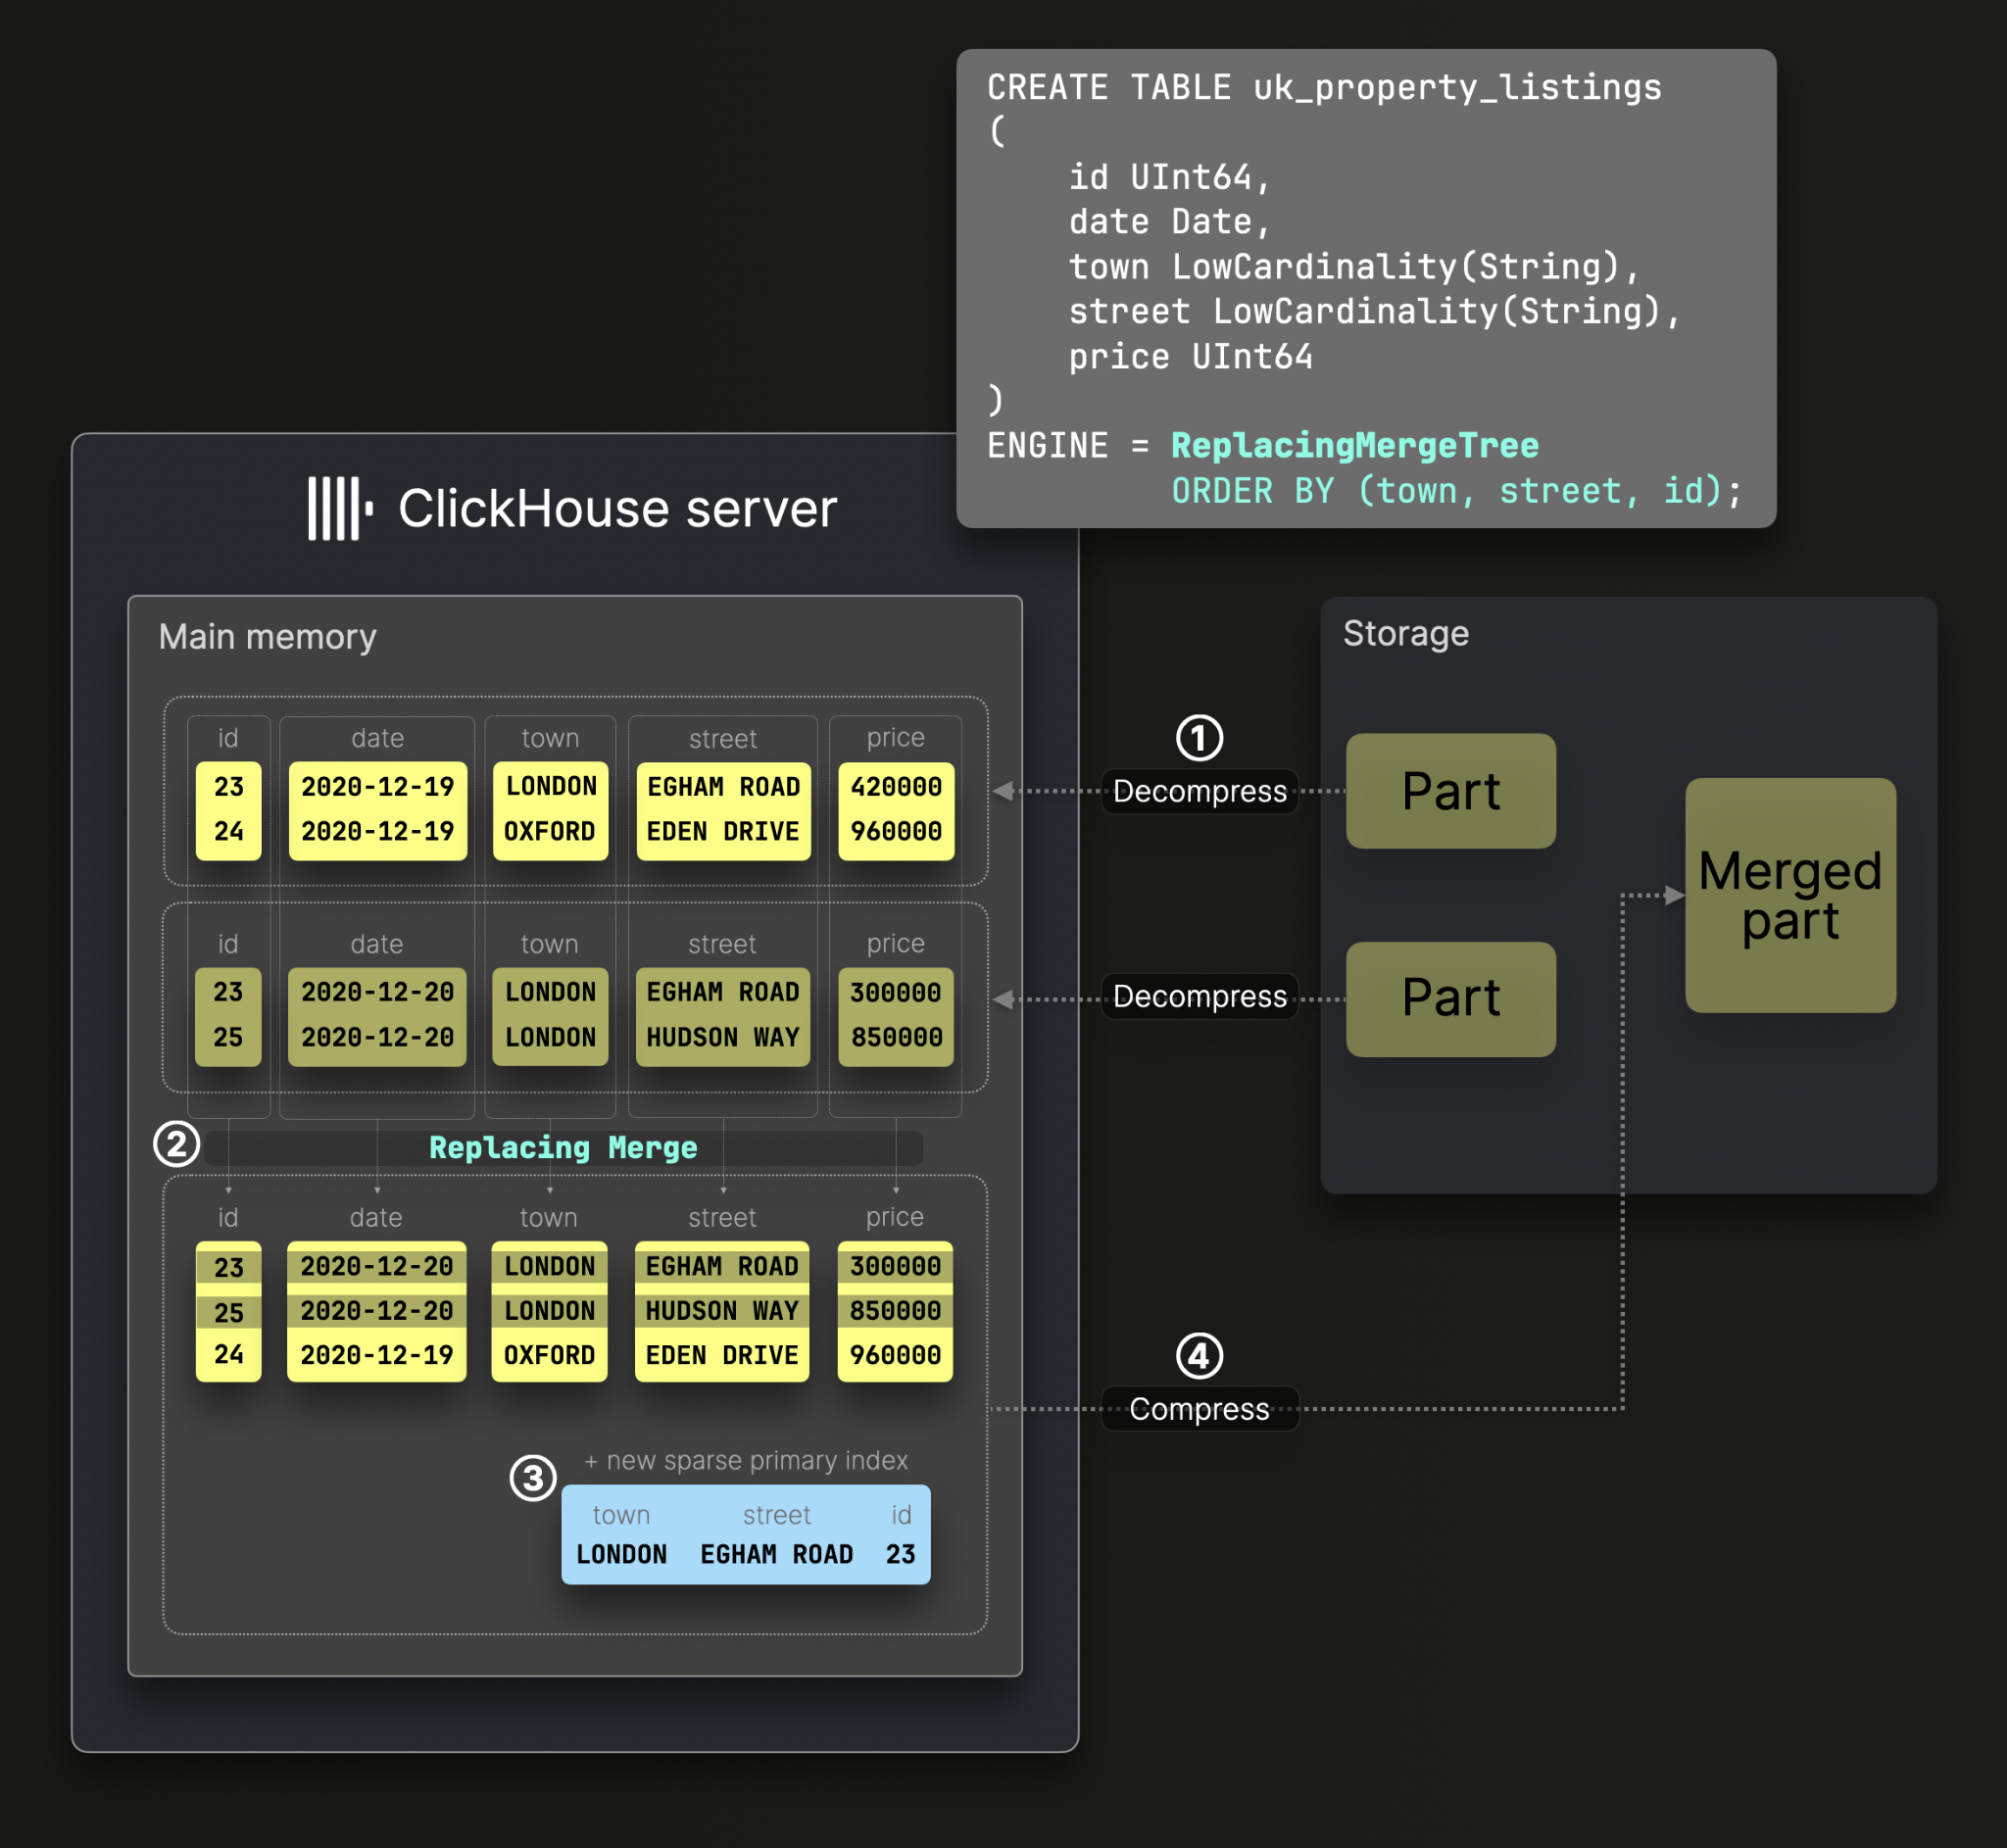
\includegraphics[width=0.82\textwidth,height=0.31\textheight,keepaspectratio]{fig2_8.png}
    }{
        \fbox{\parbox{0.9\textwidth}{\centering\vspace{0.5cm}\textbf{[Chèn Hình 2.8 -- tệp \texttt{fig2\_\allowbreak{}8.png}]}\vspace{0.5cm}}}
    }
    \caption{Hợp nhất các part của ReplacingMergeTree và giữ lại hàng theo khóa sắp xếp. Nguồn: ClickHouse Docs, ``Replacing merges''~\cite{S5, V1} $\cdot$ CC BY-NC-SA~4.0.}
    \label{fig:fig2_8}
\end{figure}

\needspace{4\baselineskip}
\noindent\textbf{Vòng đời thu hồi phân đoạn (\textit{Inactive Parts Cleanup}) và Giá trị định lượng trước thực nghiệm:} Sau khi merge nền công bố part mới đạt chuẩn bất biến ở trạng thái \texttt{active = 1}, các part nguồn bị đánh dấu \texttt{active = 0} (\textit{inactive}) và được giữ tạm theo cửa sổ bảo vệ MVCC (\texttt{old\_\allowbreak{}parts\_\allowbreak{}lifetime}) để các truy vấn đang chạy hoàn tất an toàn mà không cần khóa đọc, trước khi luồng dọn rác nền gỡ bỏ hẳn khỏi thư mục đĩa~\cite{S3, S5, S6}. Cơ chế này lý giải hai hiện tượng then chốt quan sát trong báo cáo: thứ nhất, tại thời điểm ứng dụng vừa nhận xong ACK chèn lô nhỏ, dung lượng tạm trên đĩa có thể vượt tổng kích thước logic cho tới khi merge và \textit{cleanup} kết thúc; thứ hai, vì mọi phép hợp nhất tuân thủ quy tắc cô lập phân vùng (\textit{Partition Isolation}), việc chọn đúng \texttt{ORDER BY} và \texttt{PARTITION BY} ngay từ khâu thiết kế sẽ định đoạt trực tiếp cả độ trễ cắt tỉa lẫn áp lực ghi đĩa dài hạn~\cite{S2, S9}.

\needspace{4\baselineskip}
\section{Tổng kết Chương 2 và Cầu nối sang Chương 3}
\textbf{Chương~2} đã thiết lập mô hình giải tích đầy đủ cho đường ghi bất biến, chỉ mục thưa 2~tầng và tiến trình hợp nhất nền của MergeTree. Toàn bộ các giả thuyết về thứ tự khóa, kích thước hạt và cỡ lô nạp được đưa vào kiểm chứng định lượng tại \textbf{Chương~3} trên 30~triệu dòng ClickBench.

% ==================== CHƯƠNG 3 ====================
\chapter{THỰC NGHIỆM VÀ ĐÁNH GIÁ MERGETREE}

\section{Mục tiêu, câu hỏi nghiên cứu và giả thuyết}
\textbf{Chương~3} đánh giá định lượng động cơ MergeTree trên 1~nút máy chủ ClickHouse với tải \textit{clickstream} chỉ ghi nối tiếp qua 5~khía cạnh: độ trễ truy vấn, khối lượng đọc (\texttt{read\_\allowbreak{}rows}/\texttt{read\_\allowbreak{}bytes}), chi phí chỉ mục, thông lượng nạp và áp lực merge nền. Quá trình đo cô lập hai trạng thái tải: \texttt{SELECT} trên bảng đã ổn định và \texttt{Batch INSERT} khi nạp dữ liệu; mọi số đo phản ánh thực thi nội tại tại DB, tách biệt khỏi hệ thống đầu-cuối (giải quyết tại \textbf{Chương~5}). Ba câu hỏi nghiên cứu (RQ1--RQ3) bám sát Chương~2 gồm: \textbf{RQ1 (E1)} --- ảnh hưởng thứ tự khóa \texttt{ORDER BY}; \textbf{RQ2 (E2)} --- đánh đổi độ mịn \texttt{index\_\allowbreak{}granularity}; và \textbf{RQ3 (E3)} --- tác động kích thước lô nạp lên thông lượng và hệ số merge $\Sigma r / N$ (mô hình dự báo thời gian đặt thành Hướng mở rộng tại Mục~3.6; đối chiếu PostgreSQL trình bày độc lập tại \textbf{Chương~4}). Bảng~\ref{tab:rq_mapping} tóm tắt giả thuyết kiểm chứng và ánh xạ thực nghiệm.

\begin{table}[!htb]
\centering
\scriptsize
\setlength{\tabcolsep}{4pt}
\renewcommand{\arraystretch}{1.08}
\caption{Ánh xạ câu hỏi nghiên cứu, giả thuyết kiểm chứng và thiết kế thực nghiệm}
\label{tab:rq_mapping}
\begin{tabularx}{\textwidth}{>{\bfseries\raggedright\arraybackslash}p{1.35cm} >{\raggedright\arraybackslash}p{3.85cm} >{\raggedright\arraybackslash}p{2.55cm} >{\raggedright\arraybackslash}p{2.55cm} >{\raggedright\arraybackslash}X >{\centering\arraybackslash}p{1.1cm}}
\toprule
\textbf{RQ} & \textbf{Giả thuyết kiểm chứng} & \textbf{Biến độc lập} & \textbf{Đối chứng \& Hằng số} & \textbf{Chỉ số đo lường} & \textbf{Mục} \\
\midrule
RQ1 (E1) & Khóa \texttt{ORDER BY} khớp tiền tố giảm marks/dòng đọc; nhưng giảm đọc chưa chắc giảm độ trễ tương ứng khi overhead cố định chi phối. & Thứ tự \texttt{ORDER BY}\newline ($K_0, K_1, K_2$) & $K_0 = \texttt{tuple()}$, $g = 8.192$, 1~part, 30M~dòng & \texttt{selected\_\allowbreak{}marks}, pruning, \texttt{read\_\allowbreak{}rows}/\texttt{bytes}, latency (med/IQR), nén & 3.3 \\
\addlinespace[3pt]
RQ2 (E2) & Giảm $g$ cắt bớt dòng đọc thừa ở lọc hẹp nhưng phình \texttt{primary.idx}/marks và có thể không giảm độ trễ thực tế. & \texttt{index\_\allowbreak{}granularity}\newline ($g \in \{2.048;\, 8.192;\, 32.768\}$) & Khóa $K_1$, 1~part, \texttt{index\_\allowbreak{}granularity\_\allowbreak{}bytes = 0}, 30M~dòng & \texttt{primary.idx}, \texttt{marks\_\allowbreak{}bytes}, marks chọn, \texttt{read\_\allowbreak{}rows}, latency & 3.4 \\
\addlinespace[3pt]
RQ3 (E3) & Tăng lô \texttt{Batch INSERT} giảm số part và công việc merge, nhưng tăng RAM đệm lô và chờ gom ở producer. & Cỡ lô (10k; 100k; 1M~dòng) & Tổng 30M, khóa $K_1$, merge tự nhiên & $T_{\text{ACK}}$, $Q$ (dòng/s), parts ACK/ổn định, $\Sigma r / N$, $\Sigma\text{dur}$ & 3.5 \\
\addlinespace[3pt]
Mở rộng (RQ4) & Hồi quy 1M--10M dự báo tốt xu hướng \texttt{SELECT} 30M nhưng ngoại suy tuyến tính phase nạp sẽ sai lớn do merge và RAM hẹp. & Quy mô 1M--10M $\rightarrow$ 30M & Đóng băng hệ số E1 trước holdout 30M & MAE, MAPE, tỷ lệ thực tế/dự đoán & 3.6 \\
\addlinespace[3pt]
Đối chiếu (RQ5) & MergeTree nén và quét cột vượt trội Heap + B-tree/BRIN nhưng kém ở tra cứu điểm siêu hẹp. & DBMS & 30M~dòng, W0--W4 & Latency, dung lượng, thời gian chuẩn bị, kế hoạch & Ch.~4 \\
\bottomrule
\end{tabularx}
\end{table}

\section{Dữ liệu, môi trường và phương pháp thực nghiệm}

\subsection{Dữ liệu, môi trường phần cứng và thiết lập kiểm soát}
\begin{enumerate}
    \setlength{\itemsep}{3pt}\setlength{\parskip}{0pt}
    \item[\textbf{a.}] \textbf{Nguồn dữ liệu và truy vết shard:} Sử dụng 30~tệp Parquet chuẩn từ tập \texttt{hits} của ClickBench (commit \texttt{b0b7dd8f...})~\cite{B4, B5} theo đúng thứ tự shard \texttt{0, 10, ..., 90; 1, 11, ..., 91; 2, 12, ..., 92} (1.000.000~dòng/tệp, tổng cộng 30.000.000~dòng, không nhân bản).
    \item[\textbf{b.}] \textbf{Schema 12~cột và định dạng RowBinary:} Rút gọn thành 12~cột số học/thời gian (\texttt{WatchID}, \texttt{UserID}: \texttt{Int64}; \texttt{CounterID}, \texttt{RegionID}, \texttt{ResponseEndTiming}: \texttt{Int32}; \texttt{AdvEngineID}, \texttt{IsRefresh}, \texttt{ResolutionWidth}, \texttt{ResolutionHeight}, \texttt{DontCountHits}: \texttt{Int16}; \texttt{EventDate}: \texttt{Date}; \texttt{EventTime}: \texttt{DateTime('UTC')}), xuất ra RowBinary~\cite{S18} dài đúng 44~B/dòng (1.320.000.000~B cho 30M, không chứa \texttt{NULL}).
    \item[\textbf{c.}] \textbf{Tạo mẫu hệ thống lồng nhau:} Các mẫu 1M, 3M và 10M lần lượt trích các dòng có chỉ số toàn cục chia~30 dư $< 1$, $< 3$ và $< 10$; tập 30M giữ trọn dữ liệu. Trên cả 4~quy mô đều trải đúng 17~ngày (02--31/07/2013), với số \texttt{CounterID} phân biệt đạt 1.648 / 1.687 / 1.861 / 2.113 và số \texttt{RegionID} phân biệt đạt 3.434 / 4.015 / 5.266 / 6.834. Tính toàn vẹn xác minh bằng SHA-256 trên 30/30~Parquet nguồn, 12/30~RowBinary lưu kiểm và fingerprint \texttt{count()}/\texttt{cityHash64}~\cite{M5, M6}.
\end{enumerate}

Bảng~\ref{tab:env_setup} và Bảng~\ref{tab:fixed_settings} tổng hợp 3~máy đo độc lập cùng toàn bộ tham số cố định để cô lập thuần túy cơ chế MergeTree.

\begin{table}[!htb]
\centering
\scriptsize
\renewcommand{\arraystretch}{1.08}
\caption{Tổng hợp cấu hình môi trường phần cứng và phần mềm của E1, E2 và E3}
\label{tab:env_setup}
\begin{tabularx}{\textwidth}{>{\bfseries\raggedright\arraybackslash}p{2.7cm} >{\raggedright\arraybackslash}X >{\raggedright\arraybackslash}X >{\raggedright\arraybackslash}X}
\toprule
\textbf{Thành phần} & \textbf{Máy đo E1 (\texttt{laptop1})} & \textbf{Máy đo E2 (\texttt{wsl\_\allowbreak{}xeon})} & \textbf{Máy đo E3 (\texttt{laptop\_\allowbreak{}i5})} \\
\midrule
CPU & AMD Ryzen AI~7 H~450 (8c/16t) & Intel Xeon E-2176M, 2,70~GHz (6c/12t) & Intel Core i5-11400H (6c/12t) \\
RAM WSL2 & 15,20~GiB & 15,38~GiB (không giới hạn) & 5,65~GiB \\
HĐH / Lưu trữ & Ubuntu WSL2; SSD NVMe 1~TB & Win~11 / Ubuntu 26.04.1 WSL2 (VHDX 125,2~GiB trống) & Ubuntu WSL2; SSD NVMe \\
ClickHouse & 26.10.4.207 Stable & 26.10.3.7 Stable & 26.10.3.7 Stable \\
Phạm vi & E1 (Sorting key) & E2 (Index granularity) & E3 (Batch \& Merges) \\
\bottomrule
\end{tabularx}
\end{table}

\begin{table}[!htb]
\centering
\scriptsize
\renewcommand{\arraystretch}{1.08}
\caption{Các thiết lập MergeTree và phiên làm việc giữ cố định}
\label{tab:fixed_settings}
\begin{tabularx}{\textwidth}{>{\bfseries\raggedright\arraybackslash}p{2.85cm} >{\raggedright\arraybackslash}p{4.55cm} >{\raggedright\arraybackslash}X}
\toprule
\textbf{Thành phần} & \textbf{Thiết lập cố định} & \textbf{Lý do kiểm soát} \\
\midrule
Engine \& codec & MergeTree; 12~cột; \texttt{CODEC(LZ4)}~\cite{M1} & Chuẩn hóa nén đa dụng trên toàn bộ 12~cột. \\
\addlinespace[2pt]
Phân vùng \& phụ trợ & Không \texttt{PARTITION BY}, MV, projection, skip index & Toàn bộ dữ liệu trong tháng 07/2013; tránh nhiễu ngoài khóa chính. \\
\addlinespace[2pt]
Tài nguyên & \texttt{max\_\allowbreak{}threads=4}; \texttt{max\_\allowbreak{}insert\_\allowbreak{}threads=1}; \texttt{max\_\allowbreak{}memory\_\allowbreak{}usage=2e9} & Cố định 4~luồng đọc, 1~luồng ghi và trần RAM 2~GB. \\
\addlinespace[2pt]
Granule \& định dạng & \texttt{index\_\allowbreak{}granularity\_\allowbreak{}bytes=0}; \texttt{OPTIMIZE FINAL} (E1/E2) & Cô lập $g$ theo số dòng ($360~\text{KiB} \ll 10~\text{MiB}$); E3 giữ merge tự nhiên. \\
\addlinespace[2pt]
Ghi bền \& cache & \texttt{async\_\allowbreak{}insert=0}; \texttt{fsync\_\allowbreak{}after\_\allowbreak{}insert=1}; tắt cache/\texttt{PREWHERE} & Ghi đồng bộ không trễ cache Linux; cô lập thuần túy \texttt{primary.idx}~\cite{S13}. \\
\bottomrule
\end{tabularx}
\end{table}

\FloatBarrier
\subsection{Bộ truy vấn, quy trình lặp và ranh giới phương pháp}
Cả 5~workload W0--W4 chạy \texttt{SELECT count(), sum(\allowbreak{}ResolutionWidth)} (để tránh tối ưu đếm từ \texttt{count.txt}) ở chế độ \texttt{FORMAT Null} (Bảng~\ref{tab:workloads}). Mỗi cấu hình E1/E2 qua 2~warmup + 10~lượt chính (\textit{warm-repeat}, seed đảo thứ tự \texttt{20261116}), đối chứng \texttt{read\_\allowbreak{}rows}, \texttt{read\_\allowbreak{}bytes}, độ trễ từ trình khách và \texttt{system.\allowbreak{}query\_\allowbreak{}log} (tuân thủ đơn vị nhị phân MiB/KiB cho RAM/đĩa và thập phân MB cho \texttt{read\_\allowbreak{}bytes}~\cite{M4, S10}).

\begin{table}[!htb]
\centering
\scriptsize
\renewcommand{\arraystretch}{1.08}
\caption{Bộ truy vấn W0--W4 và độ chọn lọc trên pilot 1M cũng như tập 30M}
\label{tab:workloads}
\begin{tabularx}{\textwidth}{>{\bfseries\raggedright\arraybackslash}p{1.5cm} >{\raggedright\arraybackslash}p{4.3cm} >{\raggedright\arraybackslash}p{2.7cm} >{\raggedright\arraybackslash}p{2.1cm} >{\raggedright\arraybackslash}X}
\toprule
\textbf{Workload} & \textbf{Điều kiện lọc (\texttt{WHERE})} & \textbf{Khớp (Pilot 1M)} & \textbf{Khớp (30M)} & \textbf{Vai trò đối chứng} \\
\midrule
W0 & Không lọc & 1.000.000 & 30.000.000 & Quét toàn bảng tuần tự. \\
W1 & \texttt{CounterID = 3258} & 1.294 & 38.841 & Lọc chọn lọc cao ($\approx 0{,}13\%$), tiền tố $K_1$. \\
W2 & \texttt{EventDate >= '2013-07-15' AND EventDate < '2013-07-23'} & 382.135 (E2) / 382.140 (E1) & 11.464.429 & Lọc dải 8~ngày ($\approx 38{,}2\%$), tiền tố $K_2$. \\
W3 & Kết hợp W1 và W2 & 134 & 4.012 & Lọc siêu hẹp ($\approx 0{,}013\%$) trên cả $K_1, K_2$. \\
W4 & \texttt{RegionID = 229} & 205.725 (E2) / 205.892 (E1) & 6.185.519 & Lọc cột ngoài khóa ($\approx 20{,}6\%$). \\
\bottomrule
\end{tabularx}
\end{table}

\needspace{5\baselineskip}
\noindent\textbf{Ranh giới phương pháp \& Kiểm định thống kê:} Để tránh kết luận cảm tính khi IQR chồng lấp ở cỡ mẫu $n = 10$ (E1, E2) và $n = 9$ (E3), mọi cặp đối chứng được kiểm định phi tham số Mann--Whitney~U hai phía (50.000~hoán vị trên số đo thô, $\alpha = 0{,}05$); phân vị $p_{95}$ được khảo sát riêng trên mẫu lớn $n = 200\text{--}16.795$ ở \textbf{Chương~5}. Do 3~thực nghiệm chạy trên 3~máy khác nhau và E1--E2 dùng \texttt{FORMAT Null} / tắt \texttt{PREWHERE} trên bảng hẹp 44~B trong môi trường VHDX, mọi đối chiếu độ trễ được giới hạn \textit{nghiêm ngặt trong nội bộ từng máy}; ảnh hưởng của \texttt{PREWHERE}, tuần tự hóa HTTP và cột HLL nặng được kiểm chứng tiếp tại Chương~4--5.

\section{Thực nghiệm E1 --- Khóa sắp xếp và Chỉ mục chính thưa}

\subsection{Thiết kế đối chứng, kết quả cắt tỉa và lưu trữ (Quy mô 30M)}
Thực nghiệm~E1 đối chiếu 3~biến thể khóa ($g = 8.192$): $K_0 = \texttt{tuple()}$, $K_1 = \texttt{(\allowbreak{}CounterID, EventDate)}$ và $K_2 = \texttt{(\allowbreak{}EventDate, CounterID)}$ trên các quy mô hiệu chỉnh 1M--10M và tập holdout độc lập 30M (1~active Wide part; hệ số mô hình đóng băng trước khi chạy 30~warmup + 150~lượt đo 30M). Bảng~\ref{tab:e1_results}, Hình~\ref{fig:fig3_1} và Bảng~\ref{tab:e1_storage} tổng hợp kết quả cắt tỉa ($\text{Pruning} = 1 - \texttt{selected\_\allowbreak{}marks}/\texttt{total\_\allowbreak{}marks}$), độ trễ và dung lượng lưu trữ.

\begin{table}[!htb]
\centering
\footnotesize
\renewcommand{\arraystretch}{1.12}
\caption{Kết quả cắt tỉa chỉ mục, khối lượng đọc, độ trễ và bộ nhớ trên tập 30M~dòng (E1, $g = 8.192$, máy \texttt{laptop1})}
\label{tab:e1_results}
\resizebox{\textwidth}{!}{%
\begin{tabular}{llcccccccrc}
\toprule
\textbf{Case} & \textbf{Key} & \textbf{\begin{tabular}[c]{@{}c@{}}Selected /\\Total Marks\end{tabular}} & \textbf{\begin{tabular}[c]{@{}c@{}}Pruning\\(\%)\end{tabular}} & \textbf{\begin{tabular}[c]{@{}c@{}}Estimated\\Rows\end{tabular}} & \textbf{\begin{tabular}[c]{@{}c@{}}Actual\\\texttt{read\_\allowbreak{}rows}\end{tabular}} & \textbf{\begin{tabular}[c]{@{}c@{}}Actual\\\texttt{read\_\allowbreak{}bytes}\end{tabular}} & \textbf{\begin{tabular}[c]{@{}c@{}}Server Latency\\Median ($Q_1$--$Q_3$) (ms)\end{tabular}} & \textbf{\begin{tabular}[c]{@{}c@{}}Client Latency\\Median ($Q_1$--$Q_3$) (ms)\end{tabular}} & \textbf{\begin{tabular}[c]{@{}c@{}}Speedup\\$\frac{\text{med}(T_{K_0})}{\text{med}(T_{K_i})}$\end{tabular}} & \textbf{\begin{tabular}[c]{@{}c@{}}Peak RAM\\(MiB)\end{tabular}} \\
\midrule
W0 & $K_0$ & 3.663 / 3.663 & 0,00\% & 30.000.000 & 30.000.000 & 60,00 MB & 20,0 (19,0--20,8) & 21,4 (20,5--22,5) & 1,00${\times}$ & 3,86 \\
W0 & $K_1$ & 3.663 / 3.663 & 0,00\% & 30.000.000 & 30.000.000 & 60,00 MB & 20,0 (19,3--20,0) & 20,9 (20,6--21,1) & 1,02${\times}$ & 3,98 \\
W0 & $K_2$ & 3.663 / 3.663 & 0,00\% & 30.000.000 & 30.000.000 & 60,00 MB & 20,0 (20,0--21,0) & 21,6 (21,3--21,9) & 0,99${\times}$ & 3,90 \\
\midrule
W1 & $K_0$ & 3.663 / 3.663 & 0,00\% & 30.000.000 & 30.000.000 & 180,00 MB & 26,0 (25,0--27,5) & 26,9 (26,6--28,8) & 1,00${\times}$ & 3,52 \\
W1 & $K_1$ & 6 / 3.663 & 99,84\% & 49.152 & 49.152 & 0,29 MB & 2,0 (2,0--2,0) & 3,5 (3,3--3,6) & 7,76${\times}$ & 3,35 \\
W1 & $K_2$ & 28 / 3.663 & 99,24\% & 222.080 & 222.080 & 1,33 MB & 4,0 (4,0--4,0) & 5,1 (4,8--5,3) & 5,29${\times}$ & 4,11 \\
\midrule
W2 & $K_0$ & 3.663 / 3.663 & 0,00\% & 30.000.000 & 30.000.000 & 120,00 MB & 27,5 (27,0--28,0) & 28,8 (28,7--29,2) & 1,00${\times}$ & 4,18 \\
W2 & $K_1$ & 1.756 / 3.663 & 52,06\% & 14.377.856 & 14.377.856 & 57,51 MB & 20,0 (19,3--20,0) & 20,9 (20,5--21,6) & 1,38${\times}$ & 4,20 \\
W2 & $K_2$ & 1.400 / 3.663 & 61,78\% & 11.468.800 & 11.468.800 & 45,88 MB & 14,0 (14,0--14,0) & 15,5 (15,0--15,7) & 1,86${\times}$ & 4,36 \\
\midrule
W3 & $K_0$ & 3.663 / 3.663 & 0,00\% & 30.000.000 & 30.000.000 & 240,00 MB & 30,0 (29,0--30,8) & 31,0 (29,8--32,1) & 1,00${\times}$ & 3,65 \\
W3 & $K_1$ & 2 / 3.663 & 99,95\% & 16.384 & 16.384 & 0,13 MB & 3,0 (2,3--3,8) & 4,2 (3,7--5,0) & 7,44${\times}$ & 3,41 \\
W3 & $K_2$ & 5 / 3.663 & 99,86\% & 40.960 & 40.960 & 0,33 MB & 3,5 (3,0--4,0) & 4,9 (4,3--5,2) & 6,37${\times}$ & 3,39 \\
\midrule
W4 & $K_0$ & 3.663 / 3.663 & 0,00\% & 30.000.000 & 30.000.000 & 180,00 MB & 43,0 (41,3--45,3) & 44,2 (42,7--46,4) & 1,00${\times}$ & 4,48 \\
W4 & $K_1$ & 3.663 / 3.663 & 0,00\% & 30.000.000 & 30.000.000 & 180,00 MB & 42,0 (41,3--44,8) & 43,5 (42,7--46,0) & 1,02${\times}$ & 4,70 \\
W4 & $K_2$ & 3.663 / 3.663 & 0,00\% & 30.000.000 & 30.000.000 & 180,00 MB & 43,5 (43,0--46,0) & 44,7 (44,1--47,6) & 0,99${\times}$ & 4,66 \\
\bottomrule
\end{tabular}%
}
\end{table}

\noindent\textit{(Lưu ý tính toán: Hệ số tăng tốc $\text{Speedup} = \text{median}(T_{K_0}) / \text{median}(T_{K_i})$ trong Bảng~\ref{tab:e1_results} được tính từ giá trị trung vị chưa làm tròn đến 2~chữ số thập phân ở Bảng~\ref{tab:e1_forecast} --- ví dụ tại \texttt{W1/\allowbreak{}K1}, $26{,}94 / 3{,}47 = 7{,}76{\times}$ thay vì chia số hiển thị làm tròn 1~chữ số $26{,}9 / 3{,}5 = 7{,}69{\times}$. Đối với các ca có độ trễ máy chủ làm tròn nguyên mili-giây nhỏ, báo cáo luôn đối chiếu bằng độ trễ trình khách phân giải micro-giây).}

\begin{figure}[!htb]
    \centering
    \IfFileExists{fig3_1.png}{
        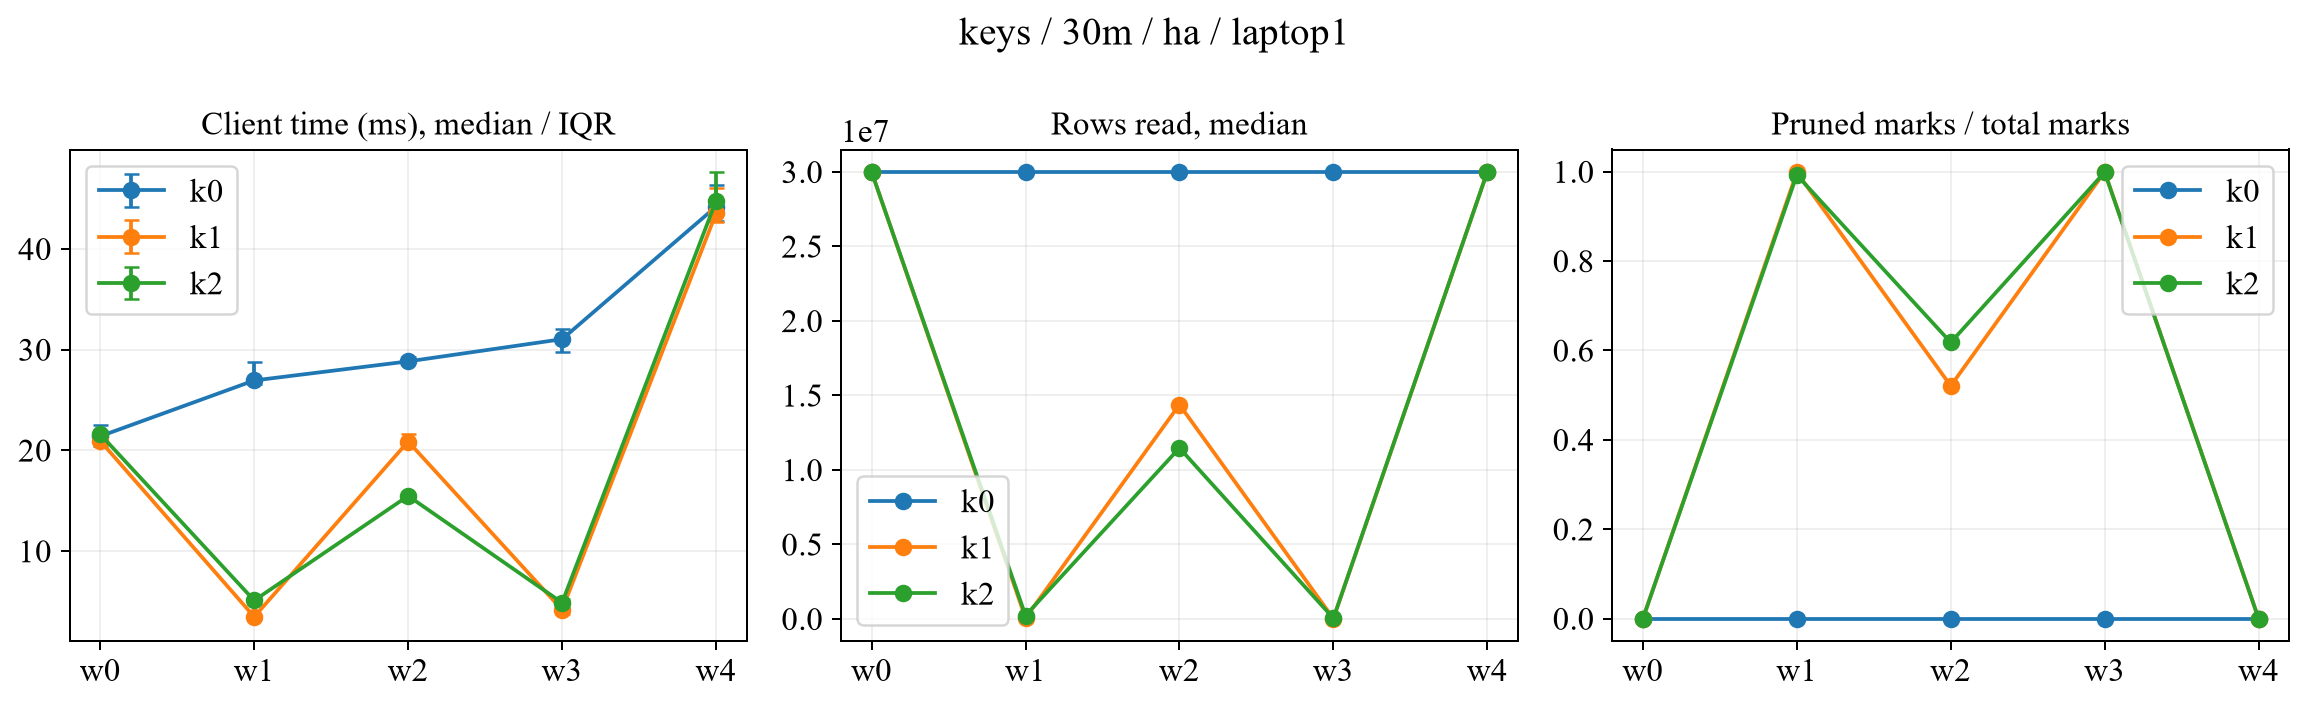
\includegraphics[width=0.94\textwidth,height=0.33\textheight,keepaspectratio]{fig3_1.png}
    }{
        \fbox{\parbox{0.9\textwidth}{\centering\vspace{0.8cm}\textbf{[Chèn Hình 3.1 -- tệp \texttt{fig3\_\allowbreak{}1.png}]}\vspace{0.8cm}}}
    }
    \caption{Biểu đồ so sánh độ trễ (Median và khoảng tứ phân vị IQR) cùng khối lượng dòng đọc (\texttt{read\_rows}) giữa $K_0$, $K_1$, $K_2$ trên các truy vấn W0--W4 ở quy mô 30M.}
    \label{fig:fig3_1}
\end{figure}

\begin{table}[!htb]
\centering
\footnotesize
\setlength{\tabcolsep}{4pt}
\renewcommand{\arraystretch}{1.1}
\caption{Dung lượng lưu trữ và tỷ lệ nén theo thứ tự khóa sắp xếp (E1, 30M~dòng, 1~active part)}
\label{tab:e1_storage}
\begin{tabularx}{\textwidth}{>{\bfseries\raggedright\arraybackslash}p{1.3cm} >{\ttfamily\raggedright\arraybackslash}p{3.3cm} >{\raggedleft\arraybackslash}p{2.9cm} >{\raggedleft\arraybackslash}p{2.8cm} >{\centering\arraybackslash}p{1.9cm} >{\raggedleft\arraybackslash}X}
\toprule
\textrm{\textbf{Biến thể Key}} & \textrm{\textbf{Định nghĩa \texttt{ORDER BY}}} & \textbf{Dung lượng chưa nén (\texttt{data\_\allowbreak{}uncompressed\_\allowbreak{}bytes})} & \textbf{Dung lượng nén trên đĩa (\texttt{bytes\_\allowbreak{}on\_\allowbreak{}disk})} & \textbf{Tỷ lệ nén} & \textbf{Kích thước \texttt{primary.idx}} \\
\midrule
$K_0$ & tuple() & 1.205.690.840~B ($\approx$~1,12~GiB) & 522.420.915~B ($\approx$~498,22~MiB) & 2,308${\times}$ (43,32\%) & 0~B \\
\addlinespace[4pt]
$K_1$ & (CounterID, EventDate) & 1.205.701.677~B ($\approx$~1,12~GiB) & 522.405.158~B ($\approx$~498,20~MiB) & 2,308${\times}$ (43,32\%) & 21.978~B ($\approx$~21,46~KiB) \\
\addlinespace[4pt]
$K_2$ & (EventDate, CounterID) & 1.205.702.687~B ($\approx$~1,12~GiB) & 522.257.659~B ($\approx$~498,06~MiB) & 2,309${\times}$ (43,31\%) & 21.978~B ($\approx$~21,46~KiB) \\
\bottomrule
\end{tabularx}
\end{table}

\noindent\textit{(Giải mã số học --- Vì sao \texttt{data\_\allowbreak{}uncompressed\_\allowbreak{}bytes} là $\approx$~1.205,7~MB thay vì 1.320,0~MB từ tệp RowBinary 44~B/dòng? Kiểm tra đối chứng trực tiếp trên bảng \texttt{system.\allowbreak{}parts\_\allowbreak{}columns} của cùng 30~triệu bản ghi với ClickHouse~26.10.4.207 xác nhận: 2~cột \texttt{Int16} có tỷ lệ giá trị mặc định \texttt{0} vượt ngưỡng \texttt{ratio\_\allowbreak{}of\_\allowbreak{}defaults\_\allowbreak{}for\_\allowbreak{}sparse\_\allowbreak{}serialization = 0,9375} --- gồm \texttt{AdvEngineID} (99,23\% bằng \texttt{0} $\rightarrow$ chỉ chiếm 779.376~B thay vì 60.000.000~B) và \texttt{IsRefresh} (chỉ chiếm 4.922.291~B thay vì 60.000.000~B) --- đã tự động kích hoạt chế độ \texttt{SerializationSparse}, loại bỏ 114.298.333~B ($\approx$~114,3~MB) phần tử \texttt{0} dư thừa ngay ở tầng giải mã chưa nén trước khi qua nén LZ4, cho ra tổng giải nén 1.205.701.667~B khớp gần như tuyệt đối với $K_1$ trong Bảng~\ref{tab:e1_storage}).}

\subsection{Phân tích và kết luận theo workload (Trả lời RQ1)}
\begin{enumerate}
    \setlength{\itemsep}{3pt}\setlength{\parskip}{0pt}
    \item \textbf{Sự phụ thuộc vào tiền tố khóa (W1, W2, W3):} Tại \textbf{W1 (\texttt{CounterID = 3258})}, khóa $K_1$ đặt \texttt{CounterID} đứng đầu đã kích hoạt \textit{Binary Search}, khoanh vùng đúng 1~dải liên tục (6~granules / 49.152~dòng, cắt tỉa 99,84\%, đạt 3,5~ms --- nhanh hơn $7{,}76{\times}$ so với $K_0$). Trái lại, $K_2$ đẩy \texttt{CounterID} xuống cột thứ hai nên buộc kích hoạt \textit{Generic Exclusion Search} qua 20~dải rời rạc (28~granules / 222.080~dòng, 5,1~ms --- vẫn nhanh hơn $K_0$ $5{,}29{\times}$ nhờ cột \texttt{EventDate} đứng trước chỉ có 17~ngày phân biệt, nhưng đọc gấp $4{,}5{\times}$ và chậm hơn $K_1$ có ý nghĩa thống kê với Mann--Whitney $U = 0{,}0$, $p = 0{,}00002$). Ngược lại ở \textbf{W2 (dải 8~ngày)}, $K_2$ quét nhị phân đọc 11,47M~dòng trong 15,5~ms ($1{,}86{\times}$), vượt trội $K_1$ chạy loại trừ tổng quát 14,38M~dòng trong 20,9~ms ($U = 0{,}0$, $p = 0{,}00002$). Ở \textbf{W3}, $K_1$ đọc ít hơn $K_2$ $2{,}5{\times}$ (2 vs 5~marks), song độ trễ 4,17 vs 4,87~ms không khác biệt ý nghĩa ($U = 32{,}0$, $p = 0{,}189 > 0{,}05$) do đều chạm ngưỡng chi phí cố định ($\approx 2\text{--}3~\text{ms}$ HTTP/pipeline).
    \item \textbf{Đối chứng W0/W4, tỷ lệ vượt lọc (\texttt{Filter} $\rightarrow$ \texttt{Aggregating}) và kiểm chứng \texttt{EXPLAIN}:} Trên W0 và lọc \texttt{RegionID} ngoài khóa (W4), cả $K_0, K_1, K_2$ đọc trọn 3.663~marks (pruning 0\%; $p \ge 0{,}248$). Đáng chú ý, tuy W4 và W1 trên $K_0$ cùng đọc chính xác 180,00~MB (30M~dòng), W4 chậm hơn $1{,}64{\times}$ (44,2 vs 26,9~ms; RAM đỉnh 4,48 vs 3,52~MiB) vì điều kiện \texttt{RegionID = 229} đẩy tới 6.185.519~dòng ($\approx 20{,}6\%$) qua toán tử tổng hợp, cao gấp $\approx 159{\times}$ so với W1 (38.841~dòng). Hiện tượng phi tuyến giữa \texttt{read\_\allowbreak{}rows} giảm $610{\times}$ và tốc độ tăng $7{,}76{\times}$ ở $K_1$/W1 xác nhận ưu thế chi phối của overhead cố định khi dữ liệu giải nén dưới vài trăm KiB. Trên cả 15/15~tổ hợp, \texttt{EXPLAIN ESTIMATE} khớp 100\% với \texttt{read\_\allowbreak{}rows} thực tế (kể cả hạt cuối bị cắt còn 896~dòng: $27 \times 8.192 + 896 = 222.080$ ở $K_2$/W1), kéo theo hệ số khuếch đại đọc thừa cấp hạt là $1{,}27{\times}$ (+26,5\%) ở $K_1$/W1 và $4{,}08{\times}$ ở $K_1$/W3 (so với $10{,}21{\times}$ ở $K_2$/W3).
    \item \textbf{Chi phí bộ nhớ chỉ mục và tính ổn định tỷ lệ nén:} Trên cả $K_1$ và $K_2$, \texttt{primary\_\allowbreak{}key\_\allowbreak{}bytes\_\allowbreak{}in\_\allowbreak{}memory} chiếm đúng $3.663 \times 6 = 21.978~\text{B}$ ($\approx 21{,}46~\text{KiB}$, bằng 0,004\% bảng). Cả 3~biến thể $K_0, K_1, K_2$ hội tụ mức nén $2{,}31{\times}$ ($\approx 498{,}06\text{--}498{,}22~\text{MiB}$ từ 1,12~GiB chưa nén) vì các trường định danh entropy cao như \texttt{WatchID}/\texttt{UserID} khó nén bằng cửa sổ LZ4 và bản Parquet gốc đã phân cụm sẵn theo trình tự thu thập. \textbf{Trả lời RQ1:} Khóa \texttt{ORDER BY} quyết định trực tiếp thuật toán tìm kiếm và phạm vi cắt tỉa; cột lọc đẳng thức lực lượng trung bình (\texttt{CounterID}) cần đứng đầu nếu ưu tiên W1/W3, ngược lại ưu tiên \texttt{EventDate} đứng đầu cho quét dải thời gian toàn bảng (W2).
\end{enumerate}

\section{Thực nghiệm E2 --- \texorpdfstring{\texttt{index\_granularity}}{index\_granularity}: thiết kế, kết quả và chi phí chỉ mục}

\subsection{Cấu hình, chuẩn bị và kiểm chứng công thức chỉ mục}
Thực nghiệm~E2 khảo sát $g \in \{2.048;\, 8.192;\, 32.768\}$ trên khóa $K_1$ (30M~dòng, 1~active Wide part, \texttt{index\_\allowbreak{}granularity\_\allowbreak{}bytes = 0}, máy \texttt{wsl\_\allowbreak{}xeon}, 30~warmup + 150~lượt khớp \texttt{system.\allowbreak{}query\_\allowbreak{}log}). Do mỗi dòng chỉ nặng 44~B (1~hạt chuẩn $\approx 360~\text{KiB} \ll 10~\text{MiB}$), đặt \texttt{index\_\allowbreak{}granularity\_\allowbreak{}bytes = 0} hoàn toàn đại diện cho mặc định sản xuất trên bảng hẹp~\cite{S2}. Trong pha chuẩn bị riêng (30~lô), thời gian nạp \texttt{ingest\_\allowbreak{}ack\_\allowbreak{}s} của $g = 2.048;\, 8.192;\, 32.768$ lần lượt là \textbf{10,749~s}, \textbf{14,384~s} và \textbf{14,872~s}, còn thời gian hợp nhất chuẩn hóa \texttt{OPTIMIZE FINAL} giảm dần từ \textbf{7.983,681~ms} xuống \textbf{7.514,693~ms} và \textbf{7.245,069~ms} (tương ứng tạo ít marks hơn khi $g$ tăng). Kiểm chứng mô hình giải tích từ Chương~2 đạt độ khớp tuyệt đối:
\begin{itemize}
    \setlength{\itemsep}{2pt}\setlength{\parskip}{0pt}
    \item \textbf{Số mốc chỉ mục ($M_{\text{est}} = \lceil N/g \rceil$):} Cho đúng \textbf{14.649}, \textbf{3.663} và \textbf{916}~marks ứng với $g \in \{2.048;\, 8.192;\, 32.768\}$, trùng khớp 100\% với \texttt{system.\allowbreak{}parts}.
    \item \textbf{Bộ nhớ RAM chỉ mục ($I_{\text{key}} = M \times 6~\text{B}$):} Tính ra đúng \textbf{87.894}, \textbf{21.978} và \textbf{5.496~B} --- khớp chính xác từng byte với \texttt{primary\_\allowbreak{}key\_\allowbreak{}bytes\_\allowbreak{}in\_\allowbreak{}memory} (Bảng~\ref{tab:e2_storage}), khẳng định \texttt{primary.idx} được lưu thành khối đệm nhị phân đóng gói liền mạch không có padding con trỏ.
    \item \textbf{Ước lượng lượng đọc ($R_{\text{est}} \approx \min(N, \texttt{selected\_\allowbreak{}marks} \times g)$):} Giải thích chính xác hạt cuối cùng bị cắt ngắn còn đúng 896~dòng ($g = 2.048;\, 8.192$) và 17.280~dòng ($g = 32.768$): trên W2 cho $6.241 \times 2.048 - 1.152 = 12.780.416$, $1.756 \times 8.192 - 7.296 = 14.377.856$, và $514 \times 32.768 - 15.488 = 16.827.264$ dòng --- khớp tuyệt đối \texttt{read\_\allowbreak{}rows} (Bảng~\ref{tab:e2_results}).
\end{itemize}

\subsection{Kết quả loại bỏ granule, độ trễ và dung lượng chỉ mục}
Bảng~\ref{tab:e2_results}, Bảng~\ref{tab:e2_storage} và Hình~\ref{fig:fig3_2} cho thấy dù hạ $g = 2.048$ giúp giảm \texttt{read\_\allowbreak{}rows} tới 62,5\% ở W3 và nâng pruning W2 lên 57,40\%, trung vị \texttt{client\_\allowbreak{}ms} gần như đi ngang (W1: 3,15--3,75~ms; W3: 3,35--3,61~ms; W2: 35,08--36,70~ms).

\begin{table}[!htb]
\centering
\footnotesize
\renewcommand{\arraystretch}{1.12}
\caption{Kết quả thực nghiệm E2 trên 30~triệu dòng với 3~mức \texttt{index\_granularity} (máy \texttt{wsl\_xeon}, $n = 10$~lượt/tổ hợp)}
\label{tab:e2_results}
\resizebox{\textwidth}{!}{%
\begin{tabular}{lcrccrr}
\toprule
\textbf{Case} & \textbf{\begin{tabular}[c]{@{}c@{}}Độ mịn\\($g$)\end{tabular}} & \textbf{\begin{tabular}[c]{@{}c@{}}\texttt{read\_\allowbreak{}rows}\\(Trung vị)\end{tabular}} & \textbf{\begin{tabular}[c]{@{}c@{}}Marks chọn /\\Tổng\end{tabular}} & \textbf{\begin{tabular}[c]{@{}c@{}}Tỷ lệ\\Pruning (\%)\end{tabular}} & \textbf{\begin{tabular}[c]{@{}c@{}}\texttt{client\_\allowbreak{}ms}\\Median (ms)\end{tabular}} & \textbf{\begin{tabular}[c]{@{}c@{}}IQR\\(ms)\end{tabular}} \\
\midrule
W0 (Full scan) & 2.048 & 30.000.000 & 14.649 / 14.649 & 0,000\% & 34,776 & 12,937 \\
W0 (Full scan) & 8.192 & 30.000.000 & 3.663 / 3.663 & 0,000\% & 38,757 & 13,210 \\
W0 (Full scan) & 32.768 & 30.000.000 & 916 / 916 & 0,000\% & 33,449 & 6,590 \\
\midrule
W1 (\texttt{CounterID}) & 2.048 & 40.960 & 20 / 14.649 & 99,863\% & 3,750 & 1,002 \\
W1 (\texttt{CounterID}) & 8.192 & 49.152 & 6 / 3.663 & 99,836\% & 3,149 & 1,000 \\
W1 (\texttt{CounterID}) & 32.768 & 98.304 & 3 / 916 & 99,672\% & 3,342 & 0,709 \\
\midrule
W2 (\texttt{EventDate}) & 2.048 & 12.780.416 & 6.241 / 14.649 & 57,396\% & 35,083 & 8,434 \\
W2 (\texttt{EventDate}) & 8.192 & 14.377.856 & 1.756 / 3.663 & 52,061\% & 35,850 & 9,918 \\
W2 (\texttt{EventDate}) & 32.768 & 16.827.264 & 514 / 916 & 43,886\% & 36,704 & 6,435 \\
\midrule
W3 (Kết hợp) & 2.048 & 6.144 & 3 / 14.649 & 99,980\% & 3,598 & 0,192 \\
W3 (Kết hợp) & 8.192 & 16.384 & 2 / 3.663 & 99,945\% & 3,347 & 0,627 \\
W3 (Kết hợp) & 32.768 & 32.768 & 1 / 916 & 99,891\% & 3,613 & 1,220 \\
\midrule
W4 (Ngoài khóa) & 2.048 & 30.000.000 & 14.649 / 14.649 & 0,000\% & 86,235 & 19,474 \\
W4 (Ngoài khóa) & 8.192 & 30.000.000 & 3.663 / 3.663 & 0,000\% & 87,399 & 13,883 \\
W4 (Ngoài khóa) & 32.768 & 30.000.000 & 916 / 916 & 0,000\% & 79,283 & 24,830 \\
\bottomrule
\end{tabular}%
}
\end{table}

\begin{table}[!htb]
\centering
\footnotesize
\setlength{\tabcolsep}{4pt}
\renewcommand{\arraystretch}{1.1}
\caption[Dung lượng dữ liệu, chỉ mục và marks trong E2 (30M dòng)]{Dung lượng dữ liệu, bộ nhớ chỉ mục và tệp marks trong E2 ($N = 30\text{M}$, 1~active Wide part, $1~\text{MiB} = 2^{20}~\text{byte}$)}
\label{tab:e2_storage}
\begin{tabularx}{\textwidth}{>{\bfseries\raggedright\arraybackslash}p{1.2cm} >{\centering\arraybackslash}p{2.15cm} >{\raggedleft\arraybackslash}p{3.15cm} >{\raggedleft\arraybackslash}p{2.3cm} >{\raggedleft\arraybackslash}p{2.35cm} >{\raggedleft\arraybackslash}X}
\toprule
$\boldsymbol{g}$ & \textbf{Marks ước tính / Thực tế} & \textbf{\texttt{primary\_\allowbreak{}key\_\allowbreak{}bytes\_\allowbreak{}in\_\allowbreak{}memory} ước tính / Thực tế (byte)} & \textbf{\texttt{marks\_\allowbreak{}bytes} trên đĩa (byte)} & \textbf{Dữ liệu nén / Toàn bảng (MiB)} & \textbf{Chênh lệch Toàn bảng $-$ Dữ liệu nén (MiB)} \\
\midrule
2.048 & 14.649 / 14.649 & 87.894 / 87.894 (85,8~KiB) & 251.092 (245,2~KiB) & 498,164 / 498,408 & $\approx$~0,244~MiB ($\approx$~250~KiB) \\
\addlinespace[4pt]
8.192 & 3.663 / 3.663 & 21.978 / 21.978 (21,5~KiB) & 103.008 (100,6~KiB) & 498,103 / 498,204 & $\approx$~0,101~MiB ($\approx$~103~KiB) \\
\addlinespace[4pt]
32.768 & 916 / 916 & 5.496 / 5.496 (5,4~KiB) & 33.161 (32,4~KiB) & 488,362 / 488,396 & $\approx$~0,034~MiB ($\approx$~35~KiB) \\
\bottomrule
\end{tabularx}
\end{table}

\begin{figure}[!htb]
    \centering
    \IfFileExists{fig3_2.png}{
        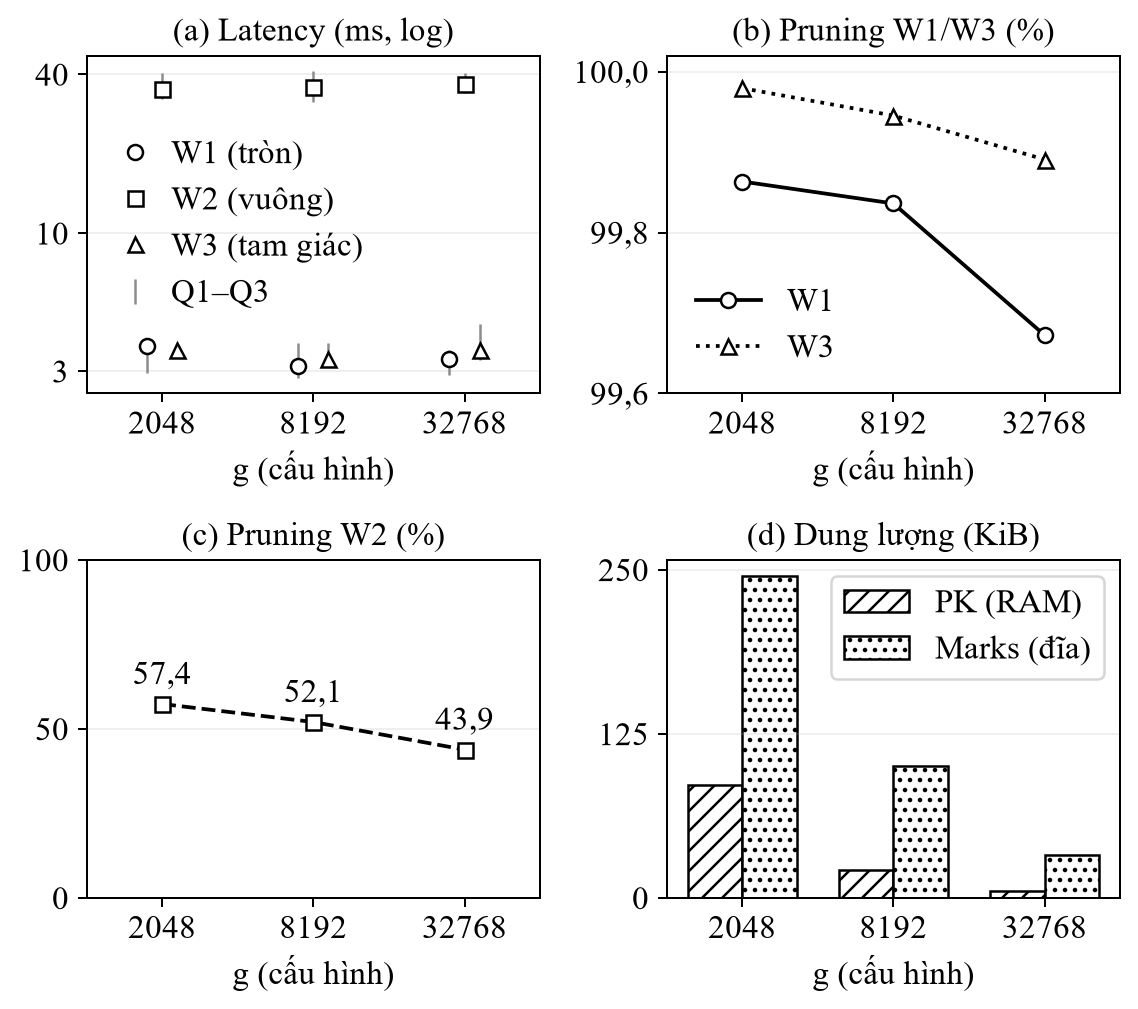
\includegraphics[width=0.86\textwidth,height=0.32\textheight,keepaspectratio]{fig3_2.png}
    }{
        \fbox{\parbox{0.9\textwidth}{\centering\vspace{0.8cm}\textbf{[Chèn Hình 3.2 -- tệp \texttt{fig3\_\allowbreak{}2.png}]}\vspace{0.8cm}}}
    }
    \caption[Biểu đồ 4 ô kết quả E2 trên máy wsl\_xeon (30M dòng)]{Biểu đồ 4~ô kết quả E2 trên máy \texttt{wsl\_xeon} ($N = 30\text{M},\; n = 10$): (a)~Trung vị \texttt{client\_ms} và khoảng $Q_1\text{--}Q_3$; (b--c)~Tỷ lệ Pruning; (d)~Dung lượng Primary index RAM và Marks đĩa.}
    \label{fig:fig3_2}
\end{figure}

\subsection{Phân tích điểm cân bằng và trả lời RQ2}
\begin{enumerate}
    \setlength{\itemsep}{3pt}\setlength{\parskip}{0pt}
    \item \textbf{Kết quả âm ở $g = 2.048$ và bằng chứng thống kê 15/15~cặp:} Giảm $g$ từ 8.192 xuống 2.048 cắt giảm \texttt{read\_\allowbreak{}rows} lần lượt 16,7\% (W1: $49.152 \rightarrow 40.960$), 11,1\% (W2: $14{,}38\text{M} \rightarrow 12{,}78\text{M}$) và 62,5\% (W3: $16.384 \rightarrow 6.144$), nhưng độ trễ trung vị lại nhích nhẹ (W1: $3{,}149 \rightarrow 3{,}750~\text{ms}$; W3: $3{,}347 \rightarrow 3{,}598~\text{ms}$). Nguyên nhân là với bộ lọc hẹp, lượng dữ liệu đọc ở cả hai mức chỉ khoảng vài chục đến vài trăm KiB đã nằm gọn trong RAM cache; ngược lại danh sách mốc phình gấp 4~lần ($14.649$ vs $3.663$ marks) làm tăng bước tìm kiếm nhị phân và số lần mở/điều phối marks (20 vs 6~marks ở W1). Hơn nữa, kiểm định Mann--Whitney~U hai phía trên cả 15/15~cặp giữa $g \in \{2.048;\, 8.192;\, 32.768\}$ qua W0--W4 đều cho $p \in [0{,}121;\, 1{,}000] > 0{,}05$ (cụ thể $g=2.048$ vs $8.192$: $p = 0{,}483 / 0{,}627 / 1{,}000 / 0{,}315 / 0{,}581$; $g=32.768$ vs $8.192$: $p = 0{,}121 / 0{,}858 / 0{,}740 / 0{,}316 / 0{,}685$), bác bỏ hoàn toàn giả thuyết thay đổi $g$ cải thiện độ trễ trên bảng hẹp 44~B. Riêng W4 chậm gấp $2{,}2{\times}$ W0 ($87{,}4$ vs $38{,}8~\text{ms}$) do phải đọc lượng dữ liệu logic lớn gấp 3~lần (180 vs 60~MB) và đẩy 6,19M~dòng qua hàm \texttt{sum()}.
    \item \textbf{Chi phí lưu trữ chỉ mục và hiện tượng nén gọn thêm 9,74~MiB ở $g = 32.768$ (Bảng~\ref{tab:e2_storage}):} Hiệu số giữa tổng dung lượng bảng và dữ liệu nén (0,244 / 0,101 / 0,034~MiB) khớp sát dung lượng \texttt{marks\_\allowbreak{}bytes} (251.092 / 103.008 / 33.161~B). Khi số marks tăng $4{\times}$, bộ nhớ RAM khóa chính tăng đúng $4{,}00{\times}$ ($21.978 \rightarrow 87.894~\text{B}$) nhưng \texttt{marks\_\allowbreak{}bytes} trên đĩa chỉ tăng $2{,}44{\times}$ nhờ nén offset liền kề. Đặc biệt, tại $g = 32.768$, dữ liệu cột nén giảm $\approx 9{,}74~\text{MiB}$ ($\approx 2\%$, còn 488,362~MiB) vì MergeTree chỉ chốt khối nén tại ranh giới granule khi dữ liệu vượt ngưỡng 64~KiB (\texttt{min\_\allowbreak{}compress\_\allowbreak{}block\_\allowbreak{}size}): hạt 32.768 gom được khối lớn hơn ($\approx 128\text{--}256~\text{KiB}$) giúp LZ4 tìm thêm nhiều mẫu lặp và giảm số lượng header khối.
    \item \textbf{Trả lời RQ2:} Với lược đồ hẹp 44~B/dòng, \textbf{$g = 8.192$} giữ điểm cân bằng tối ưu (3,15--3,35~ms; pruning W2 $> 52\%$; phụ phí chỉ 21,5~KiB RAM + 100,6~KiB marks $\approx 0{,}02\%$ bảng). Độ mịn nhỏ hơn ($g = 2.048$ hay $g = 256$ ở \textbf{Chương~5}) chỉ mang lại cải thiện thực sự khi bản ghi chứa cột rộng hoặc trạng thái phác thảo cỡ vài KiB/dòng.
\end{enumerate}

\section{Thực nghiệm E3 --- Kích thước lô INSERT và hợp nhất part nền}

\subsection{Đối chứng, dữ liệu nạp và phương pháp đo}
Thực nghiệm~E3 nạp 30M~dòng (RowBinary 44~B/dòng, khóa $K_1$, $g = 8.192$, LZ4) qua HTTP trên \texttt{laptop\_\allowbreak{}i5} (WSL2 RAM 5,65~GiB; \texttt{async\_\allowbreak{}insert = 0}, \texttt{max\_\allowbreak{}insert\_\allowbreak{}threads = 1}, \texttt{fsync\_\allowbreak{}after\_\allowbreak{}insert = 1}), giữ merge nền tự nhiên và ngưỡng \texttt{min\_\allowbreak{}bytes\_\allowbreak{}for\_\allowbreak{}wide\_\allowbreak{}part = 10~MiB} (lô 10k $\approx 0{,}42~\text{MiB}$ và 100k $\approx 4{,}20~\text{MiB}$ tạo Compact Part ban đầu rồi tự chuyển sang Wide khi gộp vượt 10~MiB; lô 1M $\approx 41{,}96~\text{MiB}$ tạo Wide Part ngay từ đầu)~\cite{S2, S9, S13}. Thí nghiệm đo luân phiên 3~đợt ${\times}$ 3~vòng = 27~lượt nạp ($n = 9$~lượt/cỡ lô) theo 3~chỉ số định nghĩa chặt chẽ~\cite{S8, M2, M3}:
\begin{itemize}
    \setlength{\itemsep}{2pt}\setlength{\parskip}{0pt}
    \item \textbf{Thời gian phản hồi $T_{\text{ACK}}$ và thông lượng $Q = N / T_{\text{ACK}}$:} Đo từ lúc gửi lệnh HTTP đầu tiên đến khi nhận xong ACK cuối (gồm đọc tệp RowBinary cục bộ giữa các lô, tách biệt khỏi công đoạn chuyển đổi Parquet hay thời gian chờ gom lô).
    \item \textbf{Trạng thái phân đoạn và hợp nhất nền:} Giám sát \texttt{system.\allowbreak{}parts} (\texttt{active = 1}) mỗi giây tại mốc sau ACK (trễ 0,007--0,479~s) và mốc ổn định (3~quan sát cách 10~s không đổi số part/merge), kết hợp trích xuất \texttt{NewPart}, tổng $\Sigma\text{duration\_ms}$ chạy song song (không cộng vào $T_{\text{ACK}}$) và hệ số đọc lặp gộp $\Sigma r / N$ từ \texttt{system.\allowbreak{}part\_\allowbreak{}log}.
    \item \textbf{Thống kê đợt đo:} Báo cáo đồng thời Trung bình ($\bar{x}$), Độ lệch chuẩn mẫu (SD) của 3~trung bình đợt, Hệ số biến thiên ($\text{CV} = \text{SD}/\bar{x} \times 100\%$) và Trung vị/IQR kèm kiểm định Mann--Whitney~U ($n = 9$).
\end{itemize}

\subsection{Kết quả nạp, hợp nhất nền và phân tích cơ chế}

\begin{table}[!htb]
\centering
\footnotesize
\renewcommand{\arraystretch}{1.15}
\caption{Kết quả nạp 30M~dòng và hoạt động hợp nhất nền theo kích thước lô (E3, máy \texttt{laptop\_i5}, $n = 9$~lượt/cỡ lô)}
\label{tab:e3_results}
\resizebox{\textwidth}{!}{%
\begin{tabular}{rcccccccc}
\toprule
\textbf{\begin{tabular}[c]{@{}c@{}}Cỡ lô\\(dòng)\end{tabular}} & \textbf{\begin{tabular}[c]{@{}c@{}}Số lệnh \texttt{INSERT}\\(\texttt{NewPart})\end{tabular}} & \textbf{\begin{tabular}[c]{@{}c@{}}$T_{\text{ACK}}$\\TB $\pm$ SD (s)\end{tabular}} & \textbf{\begin{tabular}[c]{@{}c@{}}$T_{\text{ACK}}$\\Median (IQR) (s)\end{tabular}} & \textbf{\begin{tabular}[c]{@{}c@{}}Tốc độ TB($Q$) /\\Med($Q$) (dòng/s)\end{tabular}} & \textbf{\begin{tabular}[c]{@{}c@{}}Số part\\ACK $\rightarrow$ ổn định\end{tabular}} & \textbf{\begin{tabular}[c]{@{}c@{}}Dung lượng\\ACK $\rightarrow$ ổn định (MiB)\end{tabular}} & \textbf{\begin{tabular}[c]{@{}c@{}}$\Sigma\text{dur}$ merge\\(s)\end{tabular}} & \textbf{\begin{tabular}[c]{@{}c@{}}Hệ số\\$\Sigma r / N$\end{tabular}} \\
\midrule
10.000 & 3.000 & 343,07 $\pm$ 62,35 & 345,92 (47,57) & 92.529 / 86.726 & 11,11 $\rightarrow$ 10,56 & 499,066 $\rightarrow$ 499,064 & 76,761 & 4,517 \\
100.000 & 300 & 141,54 $\pm$ 44,36 & 128,97 (76,39) & 250.358 / 232.620 & 9,00 $\rightarrow$ 9,00 & 499,763 $\rightarrow$ 499,763 & 43,596 & 2,483 \\
1.000.000 & 30 & 98,51 $\pm$ 42,96 & 83,79 (53,08) & 410.617 / 358.032 & 10,00 $\rightarrow$ 5,00 & 500,112 $\rightarrow$ 499,949 & 12,505 & 1,000 \\
\bottomrule
\end{tabular}%
}
\end{table}

\noindent\textit{(Ghi chú đo lường Bảng~\ref{tab:e3_results}: Mỗi lượt ghi đúng 3.000, 300 hoặc 30~sự kiện \texttt{NewPart} ứng với 3~cỡ lô; thời điểm lấy mẫu tại ACK trễ 0,007--0,479~s sau phản hồi cuối và bước chờ ổn định sau ACK mất 20,04--30,53~s bao gồm chu kỳ lấy mẫu 10~giây. Toàn bộ 27~lượt đều khớp tổng số dòng và giá trị băm đối chiếu~\cite{M7}).}

\subsection{Phân tích kết quả và trả lời RQ3}
\begin{enumerate}
    \setlength{\itemsep}{3pt}\setlength{\parskip}{0pt}
    \item \textbf{Lợi ích cận biên giảm dần và chi phí \texttt{fsync}:} Tăng cỡ lô từ 10.000 lên 100.000~dòng cắt giảm $T_{\text{ACK}}$ trung bình tới 58,7\% ($343{,}07 \rightarrow 141{,}54~\text{s}$); nâng tiếp lên 1.000.000~dòng giảm thêm 30,4\% (còn $98{,}51~\text{s}$), nâng tốc độ nạp $\text{TB}(Q)$ lên $4{,}44{\times}$ ($92.529 \rightarrow 410.617~\text{dòng/s}$). Việc giảm số lần gọi HTTP và ép xả đĩa \texttt{fsync\_\allowbreak{}after\_\allowbreak{}insert = 1} từ 3.000 xuống 30~lần giúp pha sắp xếp trong RAM và nén LZ4 bất biến trở thành chi phí chi phối chính~\cite{S9}.
    \item \textbf{Hợp nhất nền song song, chuyển đổi Compact$\rightarrow$Wide và đọc lặp $\Sigma r / N$:} Hệ số $\Sigma r / N$ sụt liên tiếp $4{,}517 \rightarrow 2{,}483 \rightarrow 1{,}000$ (ứng với 135,52M, 74,50M và 30,00M~lượt dòng bị đọc lại trong \texttt{MergeParts}). Dù lô 10k tạo 3.000~\texttt{NewPart}, tại thời điểm ACK chỉ còn trung bình 11,11~active parts do bể luồng nền đã merge liên hoàn suốt 5,7~phút nạp (tiêu tốn 76,761~s $\Sigma\text{dur}$), còn lô 1M giảm tối đa các tầng gộp trung gian (12,505~s)~\cite{S5}. Sau khi ổn định, cả 3~cỡ lô hội tụ dung lượng chỉ lệch 0,177\% (499,064--499,949~MiB; khác biệt nhỏ đến từ bước chuyển Compact$\rightarrow$Wide qua ngưỡng 10~MiB và số part còn lại, chưa tính inactive parts chờ xóa).
    \item \textbf{Độ phân tán VHDX ($\text{CV} = 43{,}6\%$) và kiểm định Mann--Whitney~U:} Mức chênh giữa $\text{TB}(Q) = 410.617$ và $30\text{M}/98{,}51 = 304.538~\text{dòng/s}$ phản ánh bất đẳng thức Jensen đối với $1/T$ khi phân bố thời gian giữa các đợt bị lệch trên đĩa ảo VHDX 5,65~GiB RAM. Kiểm định Mann--Whitney~U ($n = 9$) xác nhận khác biệt có ý nghĩa thống kê rất cao giữa $10\text{k} \rightarrow 100\text{k}$ ($p = 0{,}00008$) và $10\text{k} \rightarrow 1\text{M}$ ($p = 0{,}00014$), nhưng \textbf{không đạt ý nghĩa ở ngưỡng 5\% giữa $100\text{k}$ và $1\text{M}$} ($U = 23{,}0$, $p = 0{,}137 > 0{,}05$): gom lô lên 1M giảm tất định công việc merge nền ($\Sigma r / N$ giảm một nửa), song $T_{\text{ACK}}$ chưa tách biệt chắc chắn dưới dao động bộ đệm.
    \item \textbf{Đánh đổi bộ nhớ đệm \& độ trễ gom lô đầu phát (\textit{Producer Buffering Delay}):} Ba cỡ lô tương ứng payload 0,42 / 4,20 / 41,96~MiB/yêu cầu. Giả định dòng sự kiện đều với tốc độ $\lambda = 10.000~\text{dòng/s}$, thời gian trễ gom lô trung bình là $(B - 1)/(2\lambda)$ --- tới $\approx 5~\text{s}$ ở lô 100k và $\approx 50~\text{s}$ ở lô 1M --- mâu thuẫn trực tiếp với yêu cầu thời gian thực $< 1{,}5~\text{s}$ sẽ được giải quyết bằng kiến trúc luồng tại \textbf{Chương~5}.
\end{enumerate}

\section{Thời gian ước tính, số đo thực tế và giới hạn}

\subsection{Mô hình, hiệu chỉnh và đối chiếu Estimate vs. Actual}
\begin{itemize}
    \setlength{\itemsep}{3pt}
    \setlength{\parskip}{0pt}
    \setlength{\parsep}{0pt}
    \item \textbf{Mô hình SELECT (E1 Holdout trên \texttt{laptop1}):} $T_{\text{est, ms}} = \alpha + \beta \times R_{\text{est}}$ ($\alpha, \beta \ge 0$), hiệu chỉnh từ 1M, 3M, 10M với $R_{\text{est}}$ từ \texttt{EXPLAIN ESTIMATE}~\cite{S7} và đóng băng hệ số trước khi chạy holdout 30M (Bảng~\ref{tab:e1_forecast}, Hình~\ref{fig:fig3_3}a). Đường cơ sở đối chứng là ngoại suy tỷ lệ ngây thơ từ mốc 10M. Mô hình $\alpha + \beta R_{\text{est}}$ đạt $\text{MAE} = 1{,}88~\text{ms}$ (1,8829~ms) và $\text{Median APE} = 7{,}38\%$ (1,34\%--14,39\%), giảm 5,5${\times}$ sai số so với ngoại suy ngây thơ (Naive $\text{MAE} = 10{,}37~\text{ms}$, $\text{Mean APE} = 46{,}87\%$).
    \item \textbf{Mô hình nạp E3 (Phân tích hồi cứu trên \texttt{laptop\_\allowbreak{}i5}):} $T_{\text{est}}(N, B) = (N / N_0) \times \bar{T}_{\text{thử}}(N_0, B)$ ($N_0 = 1\text{M}$, $N = 30\text{M}$) giữ đủ 3~lượt pilot mỗi cỡ lô, kể cả ca đầu 10k mất 17,993~s (Bảng~\ref{tab:e3_forecast}, Hình~\ref{fig:fig3_3}b).
\end{itemize}

\begin{table}[!htb]
\centering
\scriptsize
\renewcommand{\arraystretch}{1.12}
\caption[Đối chiếu Ước tính vs. Thực đo SELECT ở quy mô Holdout 30M (E1)]{Đối chiếu Ước tính và Thực đo (Estimate vs. Actual) truy vấn \texttt{SELECT} ở quy mô Holdout 30M trong Thực nghiệm~E1 (mô hình $\alpha + \beta \cdot R_{\text{est}}$ vs. ngoại suy ngây thơ, máy \texttt{laptop1})}
\label{tab:e1_forecast}
\resizebox{\textwidth}{!}{%
\begin{tabular}{llccccccp{5.8cm}}
\toprule
\textbf{\begin{tabular}[c]{@{}l@{}}Case /\\Key\end{tabular}} & \textbf{\begin{tabular}[c]{@{}l@{}}$R_{\text{est}}$\\(dòng)\end{tabular}} & \textbf{\begin{tabular}[c]{@{}c@{}}$R^2$\\hiệu chỉnh\end{tabular}} & \textbf{\begin{tabular}[c]{@{}c@{}}Ngây thơ\\(ms)\end{tabular}} & \textbf{\begin{tabular}[c]{@{}c@{}}Ước tính\\$\alpha + \beta R$ (ms)\end{tabular}} & \textbf{\begin{tabular}[c]{@{}c@{}}Thực đo\\(ms)\end{tabular}} & \textbf{\begin{tabular}[c]{@{}c@{}}Sai số\\(ms)\end{tabular}} & \textbf{\begin{tabular}[c]{@{}c@{}}APE\\(\%)\end{tabular}} & \textbf{Nguyên nhân khả dĩ (Possible Causes)} \\
\midrule
W0 / $K_0$ & 30.000.000 & 1,000 & 33,38 & 24,33 & 21,40 & +2,93 & 13,71\% & Nén 30M tốt hơn (0,433 vs 0,460 ở 10M) + cache RAM 15,2~GiB \\
W0 / $K_1$ & 30.000.000 & 1,000 & 32,42 & 23,07 & 20,93 & +2,14 & 10,24\% & Nén 30M cải thiện + phân bổ chi phí 4~luồng hiệu quả hơn \\
W0 / $K_2$ & 30.000.000 & 0,977 & 32,50 & 23,18 & 21,59 & +1,59 & 7,38\% & Nén cải thiện và bộ đệm warm-repeat giảm chi phí thực theo dòng \\
\midrule
W1 / $K_0$ & 30.000.000 & 0,996 & 40,76 & 30,81 & 26,94 & +3,87 & 14,39\% & Quét 3~cột (180~MB) hưởng lợi mạnh từ nén 30M (2,31${\times}$) \& OS cache \\
W1 / $K_1$ & 49.152 & 0,965 & 7,10 & 3,89 & 3,47 & +0,42 & 12,11\% & Chỉ 6~marks: lệch +0,42~ms nhỏ nhưng mẫu số 3,47~ms đẩy APE \\
W1 / $K_2$ & 222.080 & 0,001 & 6,36 & 5,43 & 5,09 & +0,34 & 6,65\% & Khoảng $R_{\text{est}}$ hẹp (148k--186k), nhiễu HTTP lấn át hệ số góc ($R^2 = 0{,}001$) \\
\midrule
W2 / $K_0$ & 30.000.000 & 0,999 & 42,18 & 30,02 & 28,83 & +1,20 & 4,16\% & Ngoại suy 10M$\rightarrow$30M; phân bổ chi phí khởi tạo theo quy mô tốt hơn \\
W2 / $K_1$ & 14.377.856 & 1,000 & 31,14 & 20,59 & 20,87 & $-$0,28 & 1,34\% & Chính xác nhất (1,34\%); 134~ranges rời rạc làm thực đo nhích +0,28~ms \\
W2 / $K_2$ & 11.468.800 & 0,959 & 26,79 & 15,88 & 15,47 & +0,40 & 2,60\% & 1~range tuần tự lớn (11,47M) bám sát đường hồi quy 1M--10M \\
\midrule
W3 / $K_0$ & 30.000.000 & 0,997 & 44,15 & 31,84 & 31,03 & +0,80 & 2,59\% & Quét tuần tự 4~cột ổn định ($R^2 = 0{,}997$), nén 30M giảm nhẹ độ dốc \\
W3 / $K_1$ & 16.384 & 0,009 & 4,43 & 4,43 & 4,17 & +0,26 & 6,26\% & 8k--16k~dòng chạm trần chi phí cố định $\approx$~4~ms, nhiễu IQR chi phối $R^2$ \\
W3 / $K_2$ & 40.960 & 0,000 & 6,02 & 4,69 & 4,87 & $-$0,18 & 3,79\% & \texttt{boundary\_\allowbreak{}fit=True} ($\beta = 0$ do NNLS); 4~ranges rời rạc gây trễ nhẹ \\
\midrule
W4 / $K_0$ & 30.000.000 & 0,996 & 63,07 & 49,80 & 44,19 & +5,62 & 12,71\% & 6,19M~dòng qua Aggregating; phân bổ chi phí tốt hơn khi lên 30M \\
W4 / $K_1$ & 30.000.000 & 0,995 & 60,17 & 47,08 & 43,53 & +3,55 & 8,16\% & Cùng W4/$K_0$: nén 30M và đa luồng hạ dốc thực tế dưới đường ngoại suy \\
W4 / $K_2$ & 30.000.000 & 1,000 & 62,25 & 49,39 & 44,75 & +4,64 & 10,38\% & Sai số dương hệ thống ở các ca quét đủ 30M~dòng \\
\midrule
\textbf{Tổng hợp ($n=15$)} & Hồi quy 1M--10M $\rightarrow$ 30M & --- & \textbf{MAE 10,37} & \textbf{MAE = 1,88} & \textbf{Med APE 7,38\%} & \textbf{TB +1,82~ms} & \textbf{1,34\%--14,39\%} & \textbf{Giảm 5,5${\times}$ MAE so với ngoại suy ngây thơ (Naive Mean APE 46,87\%)} \\
\bottomrule
\end{tabular}%
}
\end{table}

\vspace{0.15cm}
\noindent\textbf{Giải thích nguyên nhân sai số mô hình SELECT~E1 (Bảng~\ref{tab:e1_forecast} \& Hình~\ref{fig:fig3_3}a):} 9~ca quét trọn 30M đều cho sai số dương nhẹ $+0{,}80\text{--}5{,}62~\text{ms}$ vì tỷ lệ nén LZ4 cải thiện dần $0{,}630 \rightarrow 0{,}433$ từ 1M lên 30M và toàn bộ bảng $\approx 522~\text{MiB}$ nằm gọn trong RAM 15,2~GiB; riêng các ca đọc ít ($K_1$/W3, $K_2$/W1, $K_2$/W3) có $R^2$ thấp do nhiễu IQR lấn át biến thiên 8k--41k~dòng, kích hoạt NNLS \texttt{boundary\_\allowbreak{}fit = True} với sai số thực $\le 0{,}42~\text{ms}$.

\begin{figure}[!htb]
    \centering
    \IfFileExists{fig3_3.png}{
        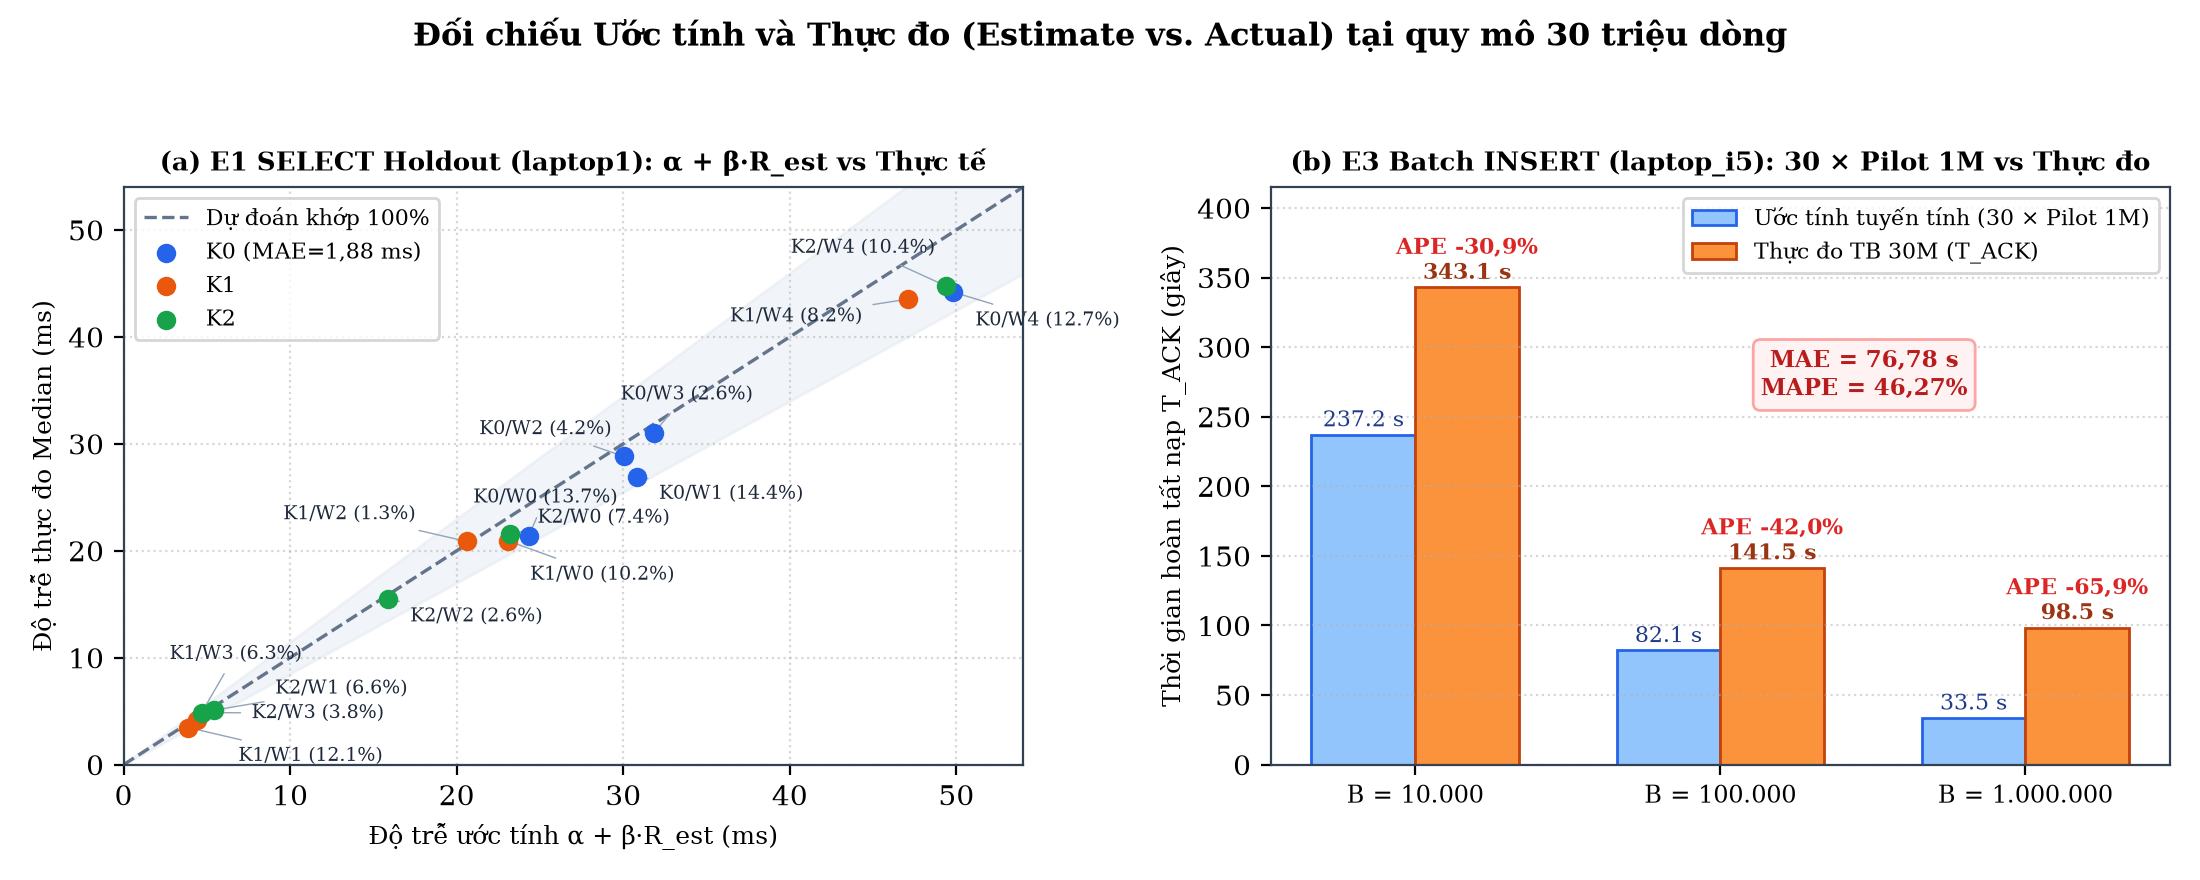
\includegraphics[width=0.94\textwidth,height=0.31\textheight,keepaspectratio]{fig3_3.png}
    }{
        \fbox{\parbox{0.9\textwidth}{\centering\vspace{0.8cm}\textbf{[Chèn Hình 3.3 -- tệp \texttt{fig3\_\allowbreak{}3.png}]}\vspace{0.8cm}}}
    }
    \caption{Đối chiếu Ước tính và Thực đo tại quy mô 30~triệu dòng: (a)~Dự báo Holdout E1 \texttt{SELECT} trên máy \texttt{laptop1}; (b)~Đối chiếu hồi cứu E3 \texttt{Batch INSERT} trên máy \texttt{laptop\_i5}.}
    \label{fig:fig3_3}
\end{figure}

\begin{table}[!htb]
\centering
\footnotesize
\renewcommand{\arraystretch}{1.15}
\caption[Đối chiếu hồi cứu thời gian nạp E3 trên máy laptop\_i5]{Đối chiếu hồi cứu thời gian nạp E3 trên máy \texttt{laptop\_i5} (từ trung bình 3~lượt pilot 1M nhân hệ số 30${\times}$ so với trung bình thực đo 9~lượt 30M ở Bảng~\ref{tab:e3_results})}
\label{tab:e3_forecast}
\begin{tabularx}{\textwidth}{>{\raggedleft\arraybackslash\bfseries}p{2.2cm} >{\raggedright\arraybackslash}X >{\raggedleft\arraybackslash}p{2.5cm} >{\raggedleft\arraybackslash}p{2.5cm} >{\raggedleft\arraybackslash}p{2.3cm} >{\raggedleft\arraybackslash}p{2.0cm}}
\toprule
\textrm{\textbf{Cỡ lô (dòng)}} & \textbf{Pilot 1M TB (s)} & \textbf{Ước tính 30${\times}$Pilot (s)} & \textbf{Thực đo 30M $T_{\text{ACK}}$ (s)} & \textbf{Sai số có dấu (s)} & \textbf{APE (\%)} \\
\midrule
10.000 & 7,905 (gồm ca đầu 17,993~s) & 237,15 & 343,07 & $-$105,93 & 30,88\% \\
\addlinespace[4pt]
100.000 & 2,737 (1~merge; $\Sigma r / N = 0{,}60$) & 82,10 & 141,54 & $-$59,44 & 42,00\% \\
\addlinespace[4pt]
1.000.000 & 1,118 (1~part; $\Sigma r / N = 0{,}00$) & 33,54 & 98,51 & $-$64,96 & 65,95\% \\
\midrule
\textbf{Tổng hợp ($n = 3$ cỡ lô)} & --- & --- & --- & \textbf{MAE = 76,78~s} & \textbf{MAPE = 46,27\%} \\
\bottomrule
\end{tabularx}
\end{table}

\vspace{0.15cm}
\noindent\textbf{Bản chất phi tuyến pha nạp E3 ($\text{MAE} = 76{,}78~\text{s}$, $\text{MAPE} = 46{,}27\%$):} Ngoại suy $30{\times}$ từ pilot 1M luôn dự báo thiếu ($-30{,}88\%$ đến $-65{,}95\%$) do merge nền ($\Sigma r/N$: $0\text{--}0{,}60 \rightarrow 1{,}000\text{--}4{,}517$), chuyển đổi Compact$\rightarrow$Wide, 300--3.000~\texttt{fsync} và áp lực bộ đệm 5,65~GiB RAM trên VHDX. Khớp hồi quy nội bộ (\textit{in-sample} 27~lượt \mbox{\texttt{Tat\_ca\_27\_case.csv}}) $T_{\text{est}}(30\text{M}, B) = \beta_0 + \beta_1 (30\text{M}/B)$ cho $\beta_0 = 106{,}44~\text{s}$, $\beta_1 = 79{,}22~\text{ms/req}$ (MAPE nội bộ 6,26\%, tiệm cận sàn đĩa ảo $\approx 106~\text{s}$); kiểm chứng ngoài mẫu đòi hỏi bổ sung các cỡ lô trung gian $B = 250\text{k}/500\text{k}$.

\subsection{Chẩn đoán bổ sung và Tổng hợp giới hạn}
Kiểm tra \texttt{EXPLAIN ANALYZE} riêng trên bảng 30M ổn định 5~parts ghi nhận 58,37~ms (full scan) và 11,48~ms (\texttt{CounterID=3258}; trong khi \texttt{SELECT} thường ghi 25~ms và 3~ms, đọc 30M và 73.728~dòng), còn ở W2 giữa lúc ACK (10~parts) và ổn định (5~parts) lượng đọc giữ ổn định ($1.788 \rightarrow 1.787$~marks). Bảng~\ref{tab:theory_vs_e3} đúc kết bằng chứng và giới hạn E3.

\begin{table}[!htb]
\centering
\scriptsize
\renewcommand{\arraystretch}{1.08}
\caption{Đối chiếu lý thuyết ở Mục~2.5 với kết quả E3}
\label{tab:theory_vs_e3}
\begin{tabularx}{\textwidth}{>{\bfseries\raggedright\arraybackslash}p{3.6cm} >{\raggedright\arraybackslash}p{4.8cm} >{\raggedright\arraybackslash}X}
\toprule
\textbf{Phát biểu lý thuyết} & \textbf{Bằng chứng hiện có} & \textbf{Kết luận và giới hạn} \\
\midrule
Hợp nhất nền (\S~2.5.1) & Nhật ký \texttt{MergeParts}, parts lúc ACK/ổn định. & Quan sát trong 1~partition đơn lẻ. \\
Cỡ lô \& tốc độ (\S~2.5.1) & $T_{\text{ACK}}$~TB: 343,07 / 141,54 / 98,51~s. & Lô lớn nạp nhanh hơn ($p \le 0{,}00014$ vs 10k). \\
Công việc merge \& đĩa & $\Sigma r/N$: $4{,}517 \rightarrow 1{,}000$; đĩa lệch 0,177\%. & Chưa đo đỉnh đĩa tạm hay byte ghi SSD. \\
Chờ gom lô \& RAM & Tính lý thuyết $(B-1)/(2\lambda)$ và cỡ payload. & Chưa đo đỉnh RAM lúc nạp hay trễ đầu-cuối. \\
Dự báo thời gian (\S~3.6) & E1: MAE 1,88~ms; E3: MAPE 46,27\%. & E1 đã kiểm holdout 30M; E3 chỉ hồi cứu. \\
\bottomrule
\end{tabularx}
\end{table}

\needspace{5\baselineskip}
\subsection{Tổng hợp liên kết cơ chế giữa E1, E2 và E3}
Kết hợp đồng thời 3~thực nghiệm có kiểm soát rút ra quy luật thiết kế liên thông cho động cơ MergeTree: (1)~\textbf{khóa sắp xếp \texttt{ORDER BY}} (E1) đóng vai trò quyết định cấp độ thô nhất --- đặt đúng cột tiền tố cho phép \textit{Binary Search} cắt tới 99,84\%--99,95\% dữ liệu và tăng tốc $7{,}76{\times}$, nhưng nếu thiếu cột đứng đầu hoặc truy vấn ngoài khóa thì mọi mật độ hạt đều vô tác dụng; (2)~\textbf{tham số \texttt{index\_\allowbreak{}granularity}} (E2) cần được nhìn cùng kích thước hàng logic và bộ lọc hai pha \texttt{PREWHERE}: trên bảng hẹp 44~B/dòng, $g = 8.192$ đã tối ưu vì 1~hạt ($\approx 360~\text{KiB}$ logic) trùng khớp dải kích thước khối nén 64~KiB--1~MiB, trong khi giảm $g$ xuống 2.048 chỉ phình danh sách \textit{marks} gấp 4~lần mà không cải thiện độ trễ ($p \ge 0{,}315$); trái lại khi mỗi dòng phình lên cỡ vài KiB ở Chương~5, hạt nhỏ giúp cắt chi phí giải nén dư thừa; và (3)~\textbf{kích thước lô ghi và hợp nhất nền} (E3) chi phối sức khỏe vận hành dài hạn: chèn lô quá nhỏ gây bão part và đẩy đọc lặp $\Sigma r / N$ lên 4,517, còn việc chuyển phần tiền tổng hợp vào Streaming MV sẽ tạo cầu nối lý tưởng cho tải luồng liên tục.

\subsection{Kiểm chứng mở rộng: Skipping Index, Projection và External Spill (máy \texttt{laptop1})}
Để lấp khoảng trống các phân hệ chưa kiểm chứng trong Bảng~\ref{tab:ch_subsystems} và giải quyết bài toán lọc cột ngoài khóa W4 (\texttt{RegionID = 229}), nghiên cứu triển khai phép đo bổ sung trên đúng 30M~dòng của \texttt{keys\_\allowbreak{}30m\_\allowbreak{}k1} tại \texttt{laptop1} (tách database cô lập \texttt{mtr\_\allowbreak{}addon\_\allowbreak{}exp}, $n = 10$~lượt \texttt{FORMAT Null}, 4~luồng~\cite{M6}). Kết quả tại Bảng~\ref{tab:ch3_ext} cho thấy ranh giới kỹ thuật sắc nét:
\begin{itemize}
    \setlength{\itemsep}{2pt}\setlength{\parskip}{0pt}
    \item \textbf{Khi nào Data Skipping Index phản tác dụng vs phát huy tác dụng:} Trên \textbf{W4 (\texttt{RegionID = 229})}, do 6.185.519~dòng (20,6\%) phân tán đều trên hầu hết các hạt của khóa \texttt{(\allowbreak{}CounterID, EventDate)}, cặp chỉ mục phụ \texttt{minmax} (2,4~KiB) và \texttt{bloom\_\allowbreak{}filter(0,01)} (1,09~MiB) chỉ loại được đúng 1/3.663~granules (\texttt{read\_\allowbreak{}rows = 29.991.808}), khiến độ trễ tăng từ 50,39 lên \textbf{60,62~ms} (+20,3\%) do tốn chi phí dò Bloom filter. Trái lại, trên giá trị chọn lọc hiếm \textbf{\texttt{RegionID = 106539}} (200~dòng), cặp skip index cắt 97,41\% bảng (\texttt{3.663 $\rightarrow$ 95} granules, 778.240~dòng), rút độ trễ \textbf{3,13${\times}$} (47,01 $\rightarrow$ \textbf{15,04~ms}).
    \item \textbf{Projection giải quyết W4 ngoài khóa:} \texttt{PROJECTION p\_\allowbreak{}reg\_\allowbreak{}order} (\texttt{SELECT * ORDER BY RegionID}) cắt được 79,36\% hạt (756/3.663) đưa W4 xuống \textbf{14,39~ms} (nhanh hơn 3,50${\times}$ nhưng tốn thêm +407,10~MiB đĩa, nâng bảng lên 905,29~MiB); trong khi \texttt{PROJECTION p\_\allowbreak{}reg\_\allowbreak{}agg} (\texttt{GROUP BY RegionID}) gom sẵn 30M dòng về đúng 6.834~hàng tổng hợp chỉ nặng \textbf{45,4~KiB} (0,009\% bảng) và giải quyết W4 trong \textbf{7,30~ms} (nhanh hơn \textbf{6,90${\times}$}).
    \item \textbf{Memory Guard \& External Spill trên 10M dòng (\texttt{GROUP BY WatchID}):} Khi đặt trần RAM \texttt{80~MB} (\texttt{76,29~MiB}) và tắt spill, ClickHouse ngắt ngay truy vấn bằng ngoại lệ \texttt{MEMORY\_\allowbreak{}LIMIT\_\allowbreak{}EXCEEDED} (cần 77,62~MiB) để bảo vệ hệ điều hành. Khi bật \texttt{max\_\allowbreak{}bytes\_\allowbreak{}before\_\allowbreak{}external\_\allowbreak{}group\_\allowbreak{}by = 60~MB} dưới trần \texttt{350~MB}, truy vấn hoàn tất an toàn trong \textbf{1.334,89~ms} (RAM đỉnh 144,70~MiB), xả \textbf{33~tệp tạm} ra đĩa (169,14~MB nén / 181,04~MB giải nén).
\end{itemize}

\begin{table}[!htb]
\centering
\small
\renewcommand{\arraystretch}{1.15}
\caption{Kiểm chứng mở rộng Skipping Index, Projection và External Spill trên \texttt{laptop1} (30M dòng W4 \& 10M \texttt{GROUP BY})}
\label{tab:ch3_ext}
\resizebox{\textwidth}{!}{%
\begin{tabular}{llcrccc}
\toprule
\textbf{Kịch bản kiểm chứng} & \textbf{Cơ chế kích hoạt} & \textbf{Đĩa phụ trợ} & \textbf{Granules / Dòng đọc} & \textbf{Client Med (IQR) (ms)} & \textbf{Server Med (ms)} & \textbf{Hệ số vs Baseline} \\
\midrule
W4 (\texttt{RegionID=229}) Base $K_1$ & Đọc tuần tự 100\% bảng & 0~B (bảng 498,20~MiB) & 3.663 / 30.000.000 & 50,39 (11,42) & 48,5 & $1{,}00{\times}$ \\
W4 + \texttt{minmax} + \texttt{bloom\_\allowbreak{}filter} & Skip Index dò cả 3.663 hạt & +1,09~MiB (+0,22\%) & 3.662 / 29.991.808 & 60,62 (17,09) & 58,5 & $0{,}83{\times}$ (Phản tác dụng) \\
W4 + \texttt{PROJECTION p\_\allowbreak{}reg\_\allowbreak{}order} & Binary Search trên \texttt{RegionID} & +407,10~MiB (+81,7\%) & 756 / 6.193.152 & 14,39 (3,90) & 12,5 & $3{,}50{\times}$ (Nhanh hơn) \\
W4 + \texttt{PROJECTION p\_\allowbreak{}reg\_\allowbreak{}agg} & Tiền tổng hợp \texttt{GROUP BY RegionID} & +45,4~KiB (0,009\%) & 1 / 6.834 & \textbf{7,30 (1,68)} & \textbf{5,5} & \textbf{6,90${\times}$ (Tối ưu nhất)} \\
\midrule
Hiếm (\texttt{RegionID=106539}, 200d) & Base $K_1$ (không Skip Index) & 0~B & 3.663 / 30.000.000 & 47,01 (11,31) & 45,5 & $1{,}00{\times}$ \\
Hiếm + \texttt{minmax} + \texttt{bloom\_\allowbreak{}filter} & Cắt tỉa 97,41\% hạt thưa & +1,09~MiB & 95 / 778.240 & \textbf{15,04 (3,35)} & \textbf{13,5} & \textbf{3,13${\times}$} \\
\midrule
10M \texttt{GROUP BY WatchID} (Guard vs Spill) & Tắt / Bật Spill (\texttt{60~MB}) & 169,14~MB (33 tệp tạm) & 10.000.000 & \textbf{Chặn OOM / 1.334,89} & 1.348 & Đỉnh RAM 144,70~MiB \\
\bottomrule
\end{tabular}%
}
\end{table}

\section{Tổng kết Chương 3}
\textbf{Chương~3} đã kiểm chứng thực nghiệm và thống kê phi tham số 3~đặc tính cốt lõi của MergeTree trong nội bộ từng máy (từ hiệu quả cắt tỉa 99,95\% của tiền tố \texttt{ORDER BY}, sự bão hòa ở $g = 8.192$ trên bảng hẹp 44~B đến lợi ích giảm $\Sigma r / N$ khi tăng lô nạp). \textbf{Chương~4} tiếp theo đối chứng trực diện MergeTree với kiến trúc Heap + B-tree/BRIN của PostgreSQL~18.6.

% ==================== CHƯƠNG 4 ====================
\chapter{ĐỐI CHIẾU MERGETREE VỚI POSTGRESQL (HEAP + B-TREE / BRIN)}

\section{Mục tiêu đối chiếu và Bản chất không tương đương vật lý}
\textbf{Chương~4} (RQ5) đối chiếu trực diện MergeTree với PostgreSQL~18.6 (Heap + BRIN/B-tree) trên cùng tập 30~triệu dòng ClickBench \texttt{hits} (12~cột) và cùng bộ W0--W4 theo 4~trụ cột: kế hoạch truy cập vật lý, dung lượng đĩa/chỉ mục, chi phí chuẩn bị và độ trễ \texttt{SELECT}~\cite{B4, B5}. Hai hệ thống đại diện cho 2~triết lý lưu trữ đối lập (Bảng~\ref{tab:ch4_physical_storage})~\cite{A1, S2, P1}: MergeTree tách từng cột nén độc lập theo hạt 8.192~dòng, duy trì \texttt{ORDER BY} qua hợp nhất nền \textit{k-way merge sort}, nạp \texttt{primary.idx} trong RAM và chỉ giải nén cột truy vấn nhờ tệp \textit{marks}; ngược lại PostgreSQL lưu trọn 12~cột trên trang Heap 8.192~B dưới \texttt{\$PGDATA/\allowbreak{}base/\allowbreak{}<db\_\allowbreak{}oid>/\allowbreak{}}, trong đó mỗi trang gánh \texttt{PageHeaderData} (24~B), \texttt{ItemIdData} (4~B/dòng), \texttt{HeapTupleHeader} (24~B/dòng) và đệm căn lề 8~byte nên tải thô 44~B/dòng nở lên $\approx 80~\text{B/dòng} \Rightarrow 2.289\text{--}2.420~\text{MiB}$ (khớp thực đo 2.417,383~MiB, sai lệch $< 1\%$), cộng chỉ mục đa cột B-tree ước lượng $\approx 200~\text{MiB}$ (thực đo 198,883~MiB)~\cite{P1, P3, P4}. Về cơ chế cắt tỉa và duy trì trật tự: chỉ mục BRIN \texttt{minmax} (\texttt{pages\_\allowbreak{}per\_\allowbreak{}range = 128}) chỉ tóm tắt biên \texttt{min/\allowbreak{}max} cho mỗi dải $128 \times 8~\text{KiB} = 1~\text{MiB}$ ($\approx 12.900$~dòng), buộc đánh dấu \textit{lossy heap blocks} và đọc \textit{recheck} toàn dải khi dữ liệu chưa phân cụm hoàn chỉnh~\cite{P2}; chỉ mục B-tree \mbox{\texttt{(CounterID, EventDate)}} trỏ trực tiếp tới từng bản ghi qua con trỏ TID nhưng phụ thuộc ước lượng độ chọn lọc của bộ tối ưu chi phí~\cite{P3, P4}; còn lệnh \texttt{CLUSTER} chỉ sắp xếp một lần không tự duy trì khi ghi nối tiếp nên thực nghiệm giữ nguyên thứ tự nạp tự nhiên rồi chạy \texttt{VACUUM (\allowbreak{}ANALYZE)} để chuẩn hóa trạng thái trang và thống kê bảng trước khi đo~\cite{P5, P6, P7}.

\begin{table}[!htb]
\centering
\scriptsize
\renewcommand{\arraystretch}{1.08}
\caption{Đối chiếu tổ chức vật lý của MergeTree và PostgreSQL Heap trong thí nghiệm}
\label{tab:ch4_physical_storage}
\begin{tabularx}{\textwidth}{>{\bfseries\raggedright\arraybackslash}p{3.0cm} >{\raggedright\arraybackslash}X >{\raggedright\arraybackslash}X}
\toprule
\textbf{Tiêu chí kiến trúc} & \textbf{ClickHouse MergeTree} & \textbf{PostgreSQL Heap (+ BRIN / B-tree)} \\
\midrule
Đơn vị lưu trữ cơ sở & Data Part bất biến tách từng tệp cột nén \texttt{.bin} + \texttt{.mrk2}~\cite{S2, S3}. & Trang cố định 8~KiB chứa đủ 12~cột mỗi dòng kèm header 24~B~\cite{P1}. \\
\addlinespace[2pt]
Thứ tự vật lý & CH1 duy trì \texttt{(\allowbreak{}CounterID, EventDate)} liên tục; CH0 giữ thứ tự gốc. & Bảng Heap chèn tự do theo luồng nhập; B-tree/BRIN là tệp tách rời. \\
\addlinespace[2pt]
Phạm vi I/O & Chỉ giải nén cột truy vấn và cắt tỉa theo hạt 8.192~dòng. & Nạp nguyên trang 8~KiB đủ 12~cột vào đệm, phát sinh đọc thừa cột. \\
\bottomrule
\end{tabularx}
\end{table}

\section{Thiết kế đối chứng và cấu hình thực nghiệm}

\subsection{Tập dữ liệu, ma trận 5 cấu hình và kiểm chứng kết quả}
Dữ liệu kế thừa bộ ClickBench 30M~dòng / 12~cột ở Mục~3.2; PostgreSQL ánh xạ sang \texttt{bigint}, \texttt{integer}, \texttt{smallint}, \texttt{date}, \texttt{timestamp with time zone} (UTC) và nạp qua \texttt{COPY BINARY}. Toàn bộ 5~cấu hình (Bảng~\ref{tab:ch4_matrix}) khớp số dòng (30.000.000), SHA-256 fingerprint 12~cột và đáp án \texttt{COUNT(*)}, \texttt{SUM(\allowbreak{}ResolutionWidth)} trên cả W0--W4.

\begin{table}[!htb]
\centering
\footnotesize
\renewcommand{\arraystretch}{1.15}
\caption{Ma trận 5~cấu hình đối chứng giữa ClickHouse và PostgreSQL (\texttt{configs/comparison.json}~\cite{M7})}
\label{tab:ch4_matrix}
\begin{tabularx}{\textwidth}{>{\bfseries\raggedright\arraybackslash}p{2.3cm} >{\raggedright\arraybackslash}p{5.5cm} >{\raggedright\arraybackslash}X}
\toprule
\textbf{Mã cấu hình} & \textbf{Tổ chức lưu trữ và chỉ mục} & \textbf{Vai trò trong thí nghiệm đối chứng} \\
\midrule
CH0 & MergeTree; \texttt{ORDER BY tuple()} & Không sắp xếp theo cột (cô lập hiệu ứng lưu trữ cột \& vector hóa thuần túy). \\
\addlinespace
CH1 & MergeTree; \texttt{ORDER BY (\allowbreak{}CounterID, EventDate)} & Cấu hình MergeTree chuẩn (kết hợp lưu trữ cột + chỉ mục thưa). \\
\addlinespace
PG0 & PostgreSQL Heap, không chỉ mục & Baseline quét bảng hàng cơ sở (\textit{Sequential Scan}). \\
\addlinespace
PG1 & PostgreSQL Heap + BRIN \texttt{(\allowbreak{}CounterID, EventDate)} & Chỉ mục tóm tắt dải khối nhẹ (\texttt{pages\_\allowbreak{}per\_\allowbreak{}range = 128}). \\
\addlinespace
PG2 & PostgreSQL Heap + B-tree \texttt{(\allowbreak{}CounterID, EventDate)} & Chỉ mục dày phổ biến nhất cho lọc bằng và lọc khoảng. \\
\bottomrule
\end{tabularx}
\end{table}

\subsection{Môi trường, cân bằng tài nguyên và phương pháp đo}
Phép đo chính (\texttt{formal43\_\allowbreak{}v3\_\allowbreak{}20261123}) chạy trên máy \texttt{wsl\_\allowbreak{}xeon} (15,38~GiB RAM), cố định cùng 4~CPU logic (0--3): ClickHouse~26.10.3.7 (\texttt{max\_\allowbreak{}threads=4}, \texttt{max\_\allowbreak{}memory\_\allowbreak{}usage=2~GB}, 1~Wide part); PostgreSQL~18.6 (\texttt{max\_\allowbreak{}parallel\_\allowbreak{}workers\_\allowbreak{}per\_\allowbreak{}gather=3} tức tối đa 4~worker, \texttt{shared\_\allowbreak{}buffers=256~MiB} dựa OS Page Cache tương đồng ClickHouse, \texttt{work\_\allowbreak{}mem=32~MiB}, \texttt{jit=off}, bật đủ WAL mặc định sản xuất)~\cite{P8}. Giao thức \texttt{crossdb-v3} chạy đảo thứ tự (seed \texttt{20261123}), 2~warmup + 10~lượt/tổ hợp (50~warmup + 250~lượt khớp 100\% đáp án \texttt{COUNT}/\texttt{SUM}); ClickHouse qua 4~kết nối HTTP tái sử dụng, PostgreSQL qua 1~kết nối Unix socket \texttt{psycopg 3.3.9} (tắt \texttt{auto-prepare}). Bảng PG1 giữ thứ tự nạp tự nhiên (không \texttt{CLUSTER}, dù shard gốc ClickBench vốn phân cụm bộ phận theo \texttt{CounterID}). Chạy riêng 1~đợt trên \texttt{laptop\_\allowbreak{}i5} (5,65~GiB RAM, \texttt{formal30m\_\allowbreak{}i5\_\allowbreak{}20261124\_\allowbreak{}105023}) để đo dung lượng và thời gian chuẩn bị khi RAM hẹp~\cite{M7}.

\section{Kết quả thực nghiệm so sánh}

\subsection{Độ trễ truy vấn theo workload và Hệ số tăng tốc}
Đợt chạy \texttt{formal43\_\allowbreak{}v3\_\allowbreak{}20261123} hoàn tất 50 lượt warmup và 250 lượt đo chính thức với đáp án khớp giữa cả 5 cấu hình (Bảng~\ref{tab:ch4_latency}, Bảng~\ref{tab:ch4_speedup}).

\begin{table}[!htb]
\centering
\footnotesize
\caption{Độ trễ \texttt{client\_ms} trên 30M dòng (máy \texttt{wsl\_xeon}): Trung vị và (IQR), đơn vị ms ($n = 10$)}
\label{tab:ch4_latency}
\resizebox{\textwidth}{!}{%
\begin{tabular}{lccccc}
\toprule
\textbf{Workload} & \textbf{CH0} & \textbf{CH1} & \textbf{PG0 (Heap)} & \textbf{PG1 (BRIN)} & \textbf{PG2 (B-tree)} \\
\midrule
W0 (Quét toàn bộ) & 44,73 (8,07) & 43,85 (8,14) & 1.553,24 (107,39) & 1.641,65 (144,07) & 1.578,53 (97,01) \\
W1 (\texttt{CounterID}) & 58,12 (9,27) & 4,90 (0,75) & 1.133,53 (151,87) & 27,35 (3,93) & 8,77 (1,67) \\
W2 (\texttt{EventDate}) & 69,41 (10,26) & 46,26 (8,74) & 1.521,25 (197,03) & 1.496,93 (61,67) & 1.547,57 (83,79) \\
W3 (Kết hợp) & 73,66 (5,02) & 5,56 (1,28) & 1.222,19 (121,78) & 21,42 (2,19) & 1,16 (0,08) \\
W4 (Ngoài khóa) & 100,88 (13,63) & 104,76 (7,38) & 1.463,29 (138,64) & 1.379,17 (51,30) & 1.405,58 (145,81) \\
\bottomrule
\end{tabular}%
}
\end{table}

\begin{table}[!htb]
\centering
\footnotesize
\caption[Hệ số tăng tốc và phần trăm giảm độ trễ của CH1 so với PostgreSQL]{Hệ số tăng tốc ($S = T_{\text{PG}} / T_{\text{CH1}}$) và phần trăm giảm độ trễ ($\Delta T\% = (T_{\text{PG}} - T_{\text{CH1}}) / T_{\text{PG}} \times 100\%$) của CH1 so với PostgreSQL}
\label{tab:ch4_speedup}
\resizebox{\textwidth}{!}{%
\begin{tabular}{lcccl}
\toprule
\textbf{Workload} & \textbf{CH1 vs PG0 (Heap cơ sở)} & \textbf{CH1 vs PG1 (BRIN)} & \textbf{CH1 vs PG2 (B-tree)} & \textbf{Kết luận ưu thế} \\
\midrule
W0 (Quét toàn bộ) & 35,42${\times}$ (+97,18\%) & 37,44${\times}$ (+97,33\%) & 36,00${\times}$ (+97,22\%) & ClickHouse vượt trội tuyệt đối \\
W1 (Lọc website) & 231,33${\times}$ (+99,57\%) & 5,58${\times}$ (+82,08\%) & 1,79${\times}$ (+44,13\%) & ClickHouse thắng cả B-tree và BRIN \\
W2 (Lọc dải ngày) & 32,88${\times}$ (+96,96\%) & 32,36${\times}$ (+96,91\%) & 33,45${\times}$ (+97,01\%) & ClickHouse vượt trội tuyệt đối \\
W3 (Lọc kết hợp hẹp) & 219,82${\times}$ (+99,55\%) & 3,85${\times}$ (+74,04\%) & $0{,}21{\times}$ ($-379{,}31\%$) & PG2 (B-tree) nhanh hơn 4,79${\times}$ \\
W4 (Lọc ngoài khóa) & 13,97${\times}$ (+92,84\%) & 13,17${\times}$ (+92,40\%) & 13,42${\times}$ (+92,55\%) & ClickHouse vượt trội tuyệt đối \\
\bottomrule
\end{tabular}%
}
\end{table}

\noindent\textit{(Ghi chú: $\Delta T\% = (T_{\text{PG}} - T_{\text{CH1}}) / T_{\text{PG}} \times 100\%$; giá trị $\Delta T\%$ lớn hơn 0 biểu thị tỷ lệ giảm độ trễ của CH1 so với cấu hình PostgreSQL tương ứng; giá trị âm tại W3 so với PG2 cho biết CH1 chậm hơn trong trường hợp lọc siêu hẹp này).}

Bảng~\ref{tab:ch4_latency}--\ref{tab:ch4_speedup} chứng minh CH1 vượt trội trên 4/5~workload: ở quét rộng và lọc ngoài khóa (W0, W2, W4), CH1 nhanh hơn PG2 $13{,}42{\times}\text{--}36{,}00{\times}$ (giảm 92,55\%--97,22\% độ trễ); ngay cả CH0 không chỉ mục vẫn thắng toàn bộ PostgreSQL $13{,}67{\times}\text{--}36{,}70{\times}$. Ở lọc website W1 (38.841~dòng), CH1 (4,90~ms) vẫn nhanh hơn PG2 B-tree $1{,}79{\times}$ (8,77~ms) và PG1 BRIN $5{,}58{\times}$ (27,35~ms). PG2 chỉ thắng duy nhất ở tra cứu điểm siêu hẹp W3 (4.012~dòng: 1,16 vs 5,56~ms, nhanh hơn $4{,}79{\times}$). \textit{(Lưu ý đối chiếu trên cùng máy \texttt{wsl\_\allowbreak{}xeon}: CH1 ở Chương~4 chậm hơn nhẹ so với E2 --- 43,85 vs 38,76~ms ở W0; 4,90/5,56 vs 3,15/3,35~ms ở W1/W3 --- vì Chương~4 trả đầy đủ payload HTTP \texttt{COUNT}/\texttt{SUM} thay cho \texttt{FORMAT Null} và chạy đồng cư với PostgreSQL; do đó Speedup chỉ tính trong nội bộ cùng đợt chạy).}

\subsection{Granule pruning, heap blocks và bằng chứng kế hoạch thực thi}
CH0 đọc trọn 3.663/3.663~marks ở cả 5~workload. Bảng~\ref{tab:ch4_explain} đối chiếu trực tiếp bằng chứng cắt tỉa của CH1 (\texttt{EXPLAIN indexes = 1}) với cây kế hoạch PostgreSQL (\texttt{EXPLAIN (\allowbreak{}ANALYZE, BUFFERS)}, tách biệt khỏi đo \texttt{client\_\allowbreak{}ms})~\cite{S7, P9}:
\begin{itemize}
    \setlength{\itemsep}{3pt}\setlength{\parskip}{0pt}
    \item \textbf{W0 (Quét toàn bảng) và W2 (Khuyết tiền tố, mật độ 38,2\%):} Cả 3~bảng PostgreSQL đều thực thi \textit{Parallel Seq Scan} ($\approx 1{,}5\text{--}1{,}6~\text{s}$). Trong cây kế hoạch, bộ lập kế hoạch chi phí đánh giá đúng mật độ lọc theo \texttt{EventDate} (11,46M/30M~dòng sau \texttt{VACUUM ANALYZE}) vượt xa ngưỡng hòa vốn I/O ngẫu nhiên nên chủ động loại bỏ cả BRIN lẫn B-tree; trái lại chỉ mục thưa CH1 vẫn kích hoạt \textit{Generic Exclusion Search} trên 17~ngày, cắt 52,061\% dữ liệu đọc (46,26~ms).
    \item \textbf{W1 (\texttt{CounterID = 3258}) và W3 (Lọc kết hợp hẹp):} Cùng sử dụng \textit{Bitmap Heap Scan}, PG1 (BRIN) chỉ khoanh được dải 128~trang nên buộc quét 2.048 và 1.664 \textit{lossy heap blocks}, phải loại bỏ tới 159.815 dòng (80,4\%) ở W1 và 157.396 dòng (97,5\%) ở W3 tại bước \textit{Rows Removed by Index Recheck}; ngược lại PG2 (B-tree) định vị chính xác 402 và 42 \textit{exact blocks} (0 dòng thừa ở \textit{recheck}), giải thích đầy đủ chênh lệch $21{,}42~\text{ms}$ vs $1{,}16~\text{ms}$ tại W3.
\end{itemize}

\begin{table}[!htb]
\centering
\scriptsize
\renewcommand{\arraystretch}{1.08}
\caption[Bằng chứng kế hoạch thực thi CH1 vs PostgreSQL (W0--W4)]{Bằng chứng kế hoạch thực thi CH1 (\texttt{EXPLAIN indexes=1}~\cite{S7}) và PostgreSQL (\texttt{EXPLAIN (ANALYZE, BUFFERS)}~\cite{P9})}
\label{tab:ch4_explain}
\resizebox{\textwidth}{!}{%
\begin{tabular}{lcclcc}
\toprule
\textbf{Workload} & \textbf{CH1: Marks (Pruning)} & \textbf{CH1: \texttt{read\_\allowbreak{}rows}} & \textbf{PG0 / PG1 (BRIN) / PG2 (B-tree): Kiểu quét} & \textbf{PG1 Heap (lossy / recheck)} & \textbf{PG2 Heap (exact / recheck)} \\
\midrule
W0 (Full) & 3.663/3.663 (0,00\%) & 30.000.000 & Parallel Seq Scan (cả 3) & --- & --- \\
W1 (\texttt{CounterID}) & 6/3.663 (99,84\%) & 49.152 & PG0: Seq; PG1/PG2: Bitmap Heap Scan & 2.048~lossy / loại 159.815 & 402~exact / loại 0 \\
W2 (\texttt{EventDate}) & 1.756/3.663 (52,06\%) & 14.377.856 & Parallel Seq Scan (bỏ qua BRIN và B-tree) & --- (Seq Scan) & --- (Seq Scan) \\
W3 (Kết hợp) & 2/3.663 (99,95\%) & 16.384 & PG0: Seq ($\approx 29{,}996\text{M}$ loại); PG1/PG2: Bitmap & 1.664~lossy / loại 157.396 & 42~exact / loại 0 \\
W4 (\texttt{RegionID}) & 3.663/3.663 (0,00\%) & 30.000.000 & Parallel Seq Scan (cả 3) & --- & --- \\
\bottomrule
\end{tabular}%
}
\end{table}

\noindent\textit{(Lưu ý đơn vị: \texttt{read\_\allowbreak{}rows} là dòng giải mã logic còn \texttt{BUFFERS} đã cộng gộp từ nút con nên không cộng lặp. Hồ sơ log/plans lưu tại nhánh \texttt{tuan/\allowbreak{}granularity} (\texttt{artifacts/\allowbreak{}tuan/\allowbreak{}wsl\_\allowbreak{}xeon/\allowbreak{}})~\cite{M7}).}

\subsection{Dung lượng dữ liệu, chỉ mục và Chi phí chuẩn bị}
Lượt \texttt{formal30m\_\allowbreak{}i5\_\allowbreak{}20261124\_\allowbreak{}105023} đo đạc kích thước vật lý các đối tượng trên đĩa (không tính WAL, nhật ký và tệp tạm, $1~\text{MiB} = 2^{20}~\text{byte} = 1.048.576~\text{byte}$)~\cite{S6, P10}. Dữ liệu đầu vào khớp 30/30~mã SHA-256 của tệp Parquet gốc và 12/30~tệp RowBinary kiểm tra cấp tệp; cả 5~cấu hình đều khớp hoàn toàn kết quả \texttt{COUNT} và \texttt{SUM(\allowbreak{}ResolutionWidth)} với máy Xeon ở W0--W4. Dung lượng ClickHouse trích từ \texttt{data\_\allowbreak{}compressed\_\allowbreak{}bytes}, \texttt{marks\_\allowbreak{}bytes} và \texttt{bytes\_\allowbreak{}on\_\allowbreak{}disk} trong \texttt{system.\allowbreak{}parts}; dung lượng PostgreSQL tính bằng \texttt{pg\_\allowbreak{}table\_\allowbreak{}size + pg\_\allowbreak{}indexes\_\allowbreak{}size}.

\begin{table}[!htb]
\centering
\footnotesize
\caption{Dung lượng dữ liệu và chỉ mục trên đĩa của 5 cấu hình (30M dòng trên \texttt{laptop\_i5}, đơn vị MiB~\cite{S6, P10})}
\label{tab:ch4_disk_size}
\resizebox{\textwidth}{!}{%
\begin{tabular}{lrrrrc}
\toprule
\textbf{Cấu hình} & \textbf{Dữ liệu bảng (MiB)} & \textbf{Chỉ mục (MiB)} & \textbf{Marks (MiB)} & \textbf{Tổng dung lượng (MiB)} & \textbf{Tỷ lệ so với CH1} \\
\midrule
CH0 & 498,126 & 0,000 & 0,098 & 498,226 & 1,00${\times}$ \\
CH1 & 498,103 & 0,002 & 0,098 & 498,204 & 1,00${\times}$ (Chuẩn nhỏ nhất) \\
PG0 (Heap) & 2.417,383 & 0,000 & --- & 2.417,383 & Lớn gấp 4,85${\times}$ \\
PG1 (BRIN) & 2.417,383 & 0,117 & --- & 2.417,500 & Lớn gấp 4,85${\times}$ \\
PG2 (B-tree) & 2.417,383 & 198,883 & --- & 2.616,266 & Lớn gấp 5,25${\times}$ \\
\bottomrule
\end{tabular}%
}
\end{table}

\noindent\textbf{Giải thích chênh lệch đĩa (tiết kiệm 80,96\%):} Tải thô RowBinary chỉ nặng 1.258,85~MiB nhưng bảng Heap PG0 phình lên 2.417,383~MiB do gánh 24~B/dòng \texttt{HeapTupleHeader} ($\approx 686{,}6~\text{MiB}$), đệm căn lề và tiêu đề trang 8~KiB không nén; ngược lại CH1 loại bỏ header dòng và nén LZ4 xuống còn 498,204~MiB (gọn hơn PG0 79,39\% và PG2 80,96\%). Cây B-tree PG2 chiếm 198,883~MiB (39,92\% cả bảng CH1), trong khi chỉ mục thưa \texttt{primary.\allowbreak{}cidx} nén trên đĩa chỉ tốn 2.071~B (0,002~MiB --- nhỏ hơn $\approx 100.700{\times}$) và RAM \texttt{primary\_\allowbreak{}key\_\allowbreak{}bytes\_\allowbreak{}in\_\allowbreak{}memory} chỉ tốn 21.978~B (0,021~MiB --- nhỏ hơn $\approx 9.490{\times}$).

\subsection{Chi phí nạp, tạo chỉ mục và chuẩn hóa dữ liệu}
Bảng~\ref{tab:ch4_prep} tổng hợp thời gian chuẩn bị đầy đủ 5~cấu hình trên \texttt{laptop\_\allowbreak{}i5} (RAM hẹp 5,65~GiB) và đối chứng CH1/PG2 từ \texttt{setup.json} trên \texttt{wsl\_\allowbreak{}xeon} (15,38~GiB)~\cite{S19, P8}.

\begin{table}[!htb]
\centering
\scriptsize
\renewcommand{\arraystretch}{1.08}
\caption{Thời gian chuẩn bị dữ liệu trên \texttt{laptop\_i5} (5,65~GiB) và \texttt{wsl\_xeon} (15,38~GiB), đơn vị giây}
\label{tab:ch4_prep}
\resizebox{\textwidth}{!}{%
\begin{tabular}{llccccc}
\toprule
\textbf{Máy đo} & \textbf{Cấu hình} & \textbf{\texttt{INSERT} / \texttt{COPY}} & \textbf{\texttt{OPTIMIZE FINAL}} & \textbf{Tạo chỉ mục} & \textbf{\texttt{VACUUM (\allowbreak{}ANALYZE)}} & \textbf{Tổng chuẩn bị (s)} \\
\midrule
\texttt{laptop\_\allowbreak{}i5} & CH0 & 86,22 & 78,38 & --- & --- & 164,60 \\
\texttt{laptop\_\allowbreak{}i5} & CH1 & 197,47 & 31,68 & --- & --- & 229,15 \\
\texttt{laptop\_\allowbreak{}i5} & PG0 & 338,79 & --- & --- & 351,49 & 690,28 \\
\texttt{laptop\_\allowbreak{}i5} & PG1 (BRIN) & 431,41 & --- & 405,65 & 317,32 & 1.154,38 \\
\texttt{laptop\_\allowbreak{}i5} & PG2 (B-tree) & 383,54 & --- & 465,30 & 329,51 & 1.178,35 \\
\midrule
\texttt{wsl\_\allowbreak{}xeon} & CH1 & 10,83 & 6,20 & --- & --- & 17,03 \\
\texttt{wsl\_\allowbreak{}xeon} & PG2 (B-tree) & 51,49 & --- & 32,54 & 21,39 & 105,42 \\
\bottomrule
\end{tabular}%
}
\end{table}

Trên \texttt{wsl\_\allowbreak{}xeon}, CH1 chỉ mất \textbf{17,03~s} (do \texttt{primary.idx} sinh đồng thời lúc ghi part) --- nhanh hơn \textbf{6,19${\times}$} so với PG2 (\textbf{105,42~s} qua 3~pha \texttt{COPY} + WAL, dựng B-tree và \texttt{VACUUM}). Dưới áp lực RAM hẹp 5,65~GiB (\texttt{laptop\_\allowbreak{}i5}), bảng Heap 2,36~GiB kết hợp chỉ mục B-tree và WAL làm tràn bộ đệm trang (\textit{page cache thrashing}) khi phải đồng thời sắp xếp ngoài đĩa để dựng cây B-tree (465,30~s) và quét toàn bảng cập nhật bản đồ hiển thị/thống kê ở bước \texttt{VACUUM (\allowbreak{}ANALYZE)} (329,51~s), đẩy PG2 lên \textbf{1.178,35~s} ($\approx 19{,}6$ phút) --- chậm hơn CH1 (\textbf{229,15~s}) tới \textbf{5,14${\times}$}. Ngược lại, MergeTree chỉ sắp xếp và nén tuần tự từng phân đoạn trong giới hạn RAM làm việc rồi sinh \texttt{primary.idx} liền mạch không phát sinh vòng đọc--ghi bổ sung riêng cho chỉ mục. \textit{(Lưu ý: thời gian chuẩn bị là 1~lượt chạy dựng bảng, chưa tách đo riêng ảnh hưởng \texttt{fsync} vs WAL).}

\section{Phân tích đánh đổi chuyên sâu và Bài toán hòa vốn}
\needspace{4\baselineskip}
\noindent\textbf{Giải mã cơ chế, Điểm hòa vốn và Giới hạn so sánh:}
\begin{enumerate}
    \setlength{\itemsep}{2pt}\setlength{\parskip}{0pt}
    \item \textbf{Đọc cột SIMD vs trang Heap (W0, W2, W4):} Ở W0, CH1 chỉ giải nén đúng cột \texttt{ResolutionWidth.bin} ($\approx 57{,}22~\text{MiB}$ logic) trong 43,85~ms, trong khi PostgreSQL phải quét trọn 2.417,38~MiB Heap (1.553--1.642~ms, chậm hơn $35{,}4\text{--}37{,}4{\times}$). Tương tự ở W4 (ngoài khóa), chỉ đọc 2~cột ($\approx 171{,}66~\text{MiB}$) giúp CH1 nhanh hơn PG2 $13{,}42{\times}$.
    \item \textbf{Điểm giao cắt Chỉ mục thưa vs B-tree (W1, W3):} Tại W1 (38.841~dòng khớp), PG2 đọc rải rác 402~trang Heap ($\approx 3{,}14~\text{MiB}$, 8,77~ms), còn CH1 đọc tuần tự 6~granules (49.152~dòng $\approx 0{,}28~\text{MiB}$, 4,90~ms). Chỉ khi lọc siêu hẹp còn 4.012~dòng tại W3, PG2 mới chạm đúng 42~\textit{exact blocks} đạt 1,16~ms, vượt qua CH1 bị giới hạn bởi đọc thừa 2~granules (16.384~dòng) và sàn cố định pipeline (5,56~ms). Ở W2 (khuyết tiền tố), \textit{Generic Exclusion} cắt 52,06\% bảng cho CH1 (46,26~ms) trong khi B-tree/BRIN đều rớt về \textit{Seq Scan} ($\approx 1{,}5~\text{s}$).
    \item \textbf{Bài toán điểm hòa vốn trên \texttt{wsl\_\allowbreak{}xeon} (Bảng~\ref{tab:ch4_latency} \& \ref{tab:ch4_prep}):} Chênh lệch chuẩn bị là $\Delta T_{\text{prep}} = 105{,}42 - 17{,}03 = 88{,}39~\text{s}$ (kèm 2.118,06~MiB đĩa dư đo trên i5). Xét riêng kịch bản nơi PG2 thắng (W3 tiết kiệm $\Delta T_{\text{W3}} = 5{,}56 - 1{,}16 = 4{,}40~\text{ms}$):
    \[
        N_{\text{hòa vốn}}(\text{W3}) = \frac{\Delta T_{\text{prep}}}{\Delta T_{\text{W3}}} = \frac{88{,}39}{0{,}00440} \approx 2{,}0 \times 10^4~\text{truy vấn (ước lượng điểm } 20.089\text{)}
    \]
    Vì $\Delta T_{\text{prep}}$ lấy từ $n = 1$ trên VHDX, ngưỡng $\sim 20.000$~truy vấn chỉ mang ý nghĩa bậc độ lớn trên bảng ít biến động; ngược lại ở mọi tải phân tích W0, W1, W2, W4, CH1 có lợi ròng ngay từ $N = 1$.
    \item \textbf{Khung quyết định định tuyến truy vấn từ bằng chứng W0--W4:} Thực nghiệm phân ranh giới rõ ràng cho hệ thống tích hợp: mọi truy vấn quét rộng, tổng hợp nhiều cột/nhiều ngày hoặc lọc ngoài khóa chính (W0, W1, W2, W4 --- nhanh hơn $1{,}79{\times}\text{--}36{,}00{\times}$) phải định tuyến sang MergeTree; ngược lại PostgreSQL B-tree chỉ nên giữ lại cho các tra cứu điểm siêu hẹp $< 5.000$~dòng kết hợp cập nhật/giao dịch trực tuyến kiểu W3 ($1{,}16~\text{ms}$ vs $5{,}56~\text{ms}$).
\end{enumerate}

\needspace{5\baselineskip}
\noindent\textbf{Ngữ nghĩa chỉ số \& Giới hạn phạm vi so sánh:} ClickHouse báo cáo \texttt{read\_\allowbreak{}rows}/\texttt{read\_\allowbreak{}bytes} ở mức giải mã logic, còn PostgreSQL \texttt{EXPLAIN (\allowbreak{}ANALYZE, BUFFERS)} đã cộng gộp bộ đệm từ nút con nên không cộng lặp~\cite{S10, P9}. Thiết lập \texttt{shared\_\allowbreak{}buffers = 256~MiB} ở PostgreSQL nhằm để cả hai hệ thống cùng khai thác 15,38~GiB OS Page Cache cho dữ liệu ấm (với 2,42~GiB Heap nằm trọn trong RAM khi chạy lặp \textit{warm-repeat}), song phép đo vẫn giữ bất đối xứng giao thức (CH 4~HTTP vs PG 1~Unix socket \texttt{psycopg}) và chỉ đo trên 1~nút. Đối với kiểm định thống kê trên \texttt{wsl\_\allowbreak{}xeon}: bộ log \texttt{crossdb-v3} hoàn chỉnh lưu ngoại tuyến từ đợt chạy chính nên bảng tổng hợp PostgreSQL giữ Trung vị/IQR ($n = 10$ với khoảng IQR hoàn toàn tách biệt), còn Mục~4.5 ngay sau đây bổ sung kiểm định Mann--Whitney~U đầy đủ khi đối chứng với DuckDB trên \texttt{laptop1}. Vì $\Delta T_{\text{prep}}$ đo từ $n = 1$ trên VHDX, điểm hòa vốn $N \approx 20.089$ chỉ có giá trị bậc độ lớn; phần định vị Druid và Elasticsearch ở Bảng~\ref{tab:dbms_positioning} dựa trên phân tích kiến trúc tài liệu kỹ thuật.

\section{Đối chứng bổ sung cùng hệ cột: ClickHouse MergeTree vs DuckDB~2.0.1}
Để trả lời câu hỏi trọng tâm \textit{liệu ClickHouse chỉ thắng vì lưu trữ hướng cột hay có đặc tính kiến trúc riêng biệt ngay cả trước một động cơ cột hiện đại khác}, nghiên cứu chạy thêm đối chứng trực diện trên chính máy \texttt{laptop1} (\texttt{15,2~GiB RAM}) giữa ClickHouse~26.10.4.207 (\texttt{CH0: tuple()}, \texttt{CH1: ORDER BY (\allowbreak{}CounterID, EventDate)}) và \textbf{DuckDB~2.0.1} (\texttt{DUCK0} nạp tự nhiên chưa sắp xếp và \texttt{DUCK1} tạo bằng \texttt{ORDER BY (\allowbreak{}CounterID, EventDate)} để tối ưu Zone Maps từng Row Group 122.880~dòng) trên trọn 30M~dòng và cùng bộ W0--W4 (cố định \texttt{threads=4}, giới hạn RAM 2~GB, 2~warmup + 10~lượt xáo trộn theo seed \texttt{20261116}, cả 4~cấu hình cùng trả đúng cặp 2~số nguyên \texttt{matched, checksum} khớp 100\% kết quả; kiểm định Mann--Whitney~U 50.000 hoán vị~\cite{M6}).

\begin{table}[!htb]
\centering
\scriptsize
\renewcommand{\arraystretch}{1.12}
\caption[Đối chứng 30M dòng giữa ClickHouse MergeTree và DuckDB 2.0.1 trên máy laptop1]{Đối chứng cùng hệ cột 30M dòng trên \texttt{laptop1}: ClickHouse~26.10.4.207 (\texttt{CH0/CH1}, HTTP JSON) vs DuckDB~2.0.1 (\texttt{DUCK0/DUCK1}, nội tiến trình), đơn vị ms ($n = 10$)}
\label{tab:ch4_duckdb}
\resizebox{\textwidth}{!}{%
\begin{tabular}{lccccc}
\toprule
\textbf{Chỉ số / Workload} & \textbf{CH0 (\texttt{tuple()})} & \textbf{CH1 (\texttt{CounterID, EventDate})} & \textbf{DUCK0 (Tự nhiên)} & \textbf{DUCK1 (\texttt{CounterID, EventDate})} & \textbf{Kiểm định CH1 vs DUCK1} \\
\midrule
Dung lượng đĩa (MiB) & 498,22 & \textbf{498,20 (Gọn nhất)} & 599,26 (+20,3\%) & 571,76 (+14,8\%) & Parquet 12~cột: 517,74~MiB \\
Thời gian dựng / sắp xếp & --- & --- & 4,80~s (từ Parquet) & 5,60~s (từ Parquet) & CH1 sinh chỉ mục trong 17,0~s (Xeon) \\
\midrule
W0 (Quét toàn bộ) & 27,31 (1,59) & 27,04 (2,66) [srv 24,5] & 29,92 (2,90) & 25,23 (2,60) & $U = 29{,}0$, $p = 0{,}123$ (Hòa thống kê) \\
W1 (\texttt{CounterID=3258}) & 34,55 (3,76) & 8,65 (1,46) [srv 6,0] & 4,25 (0,41) & \textbf{3,23 (0,64)} & $U = 0{,}0$, $p = 0{,}00002$ (DuckDB nhanh) \\
W2 (\texttt{EventDate} 8d) & 38,33 (3,76) & 27,01 (3,33) [srv 25,0] & 25,38 (2,64) & \textbf{16,86 (1,18)} & $U = 0{,}0$, $p = 0{,}00002$ (vs DUCK0 hòa $p=0{,}393$) \\
W3 (Kết hợp hẹp) & 38,17 (4,21) & 8,82 (2,28) [srv 6,5] & 5,04 (0,41) & \textbf{3,36 (0,73)} & $U = 0{,}0$, $p = 0{,}00002$ (DuckDB nhanh) \\
W4 (\texttt{RegionID=229}) & 51,57 (9,46) & 52,96 (4,57) [srv 51,0] & 37,31 (6,32) & 33,13 (3,31) & $U = 0{,}0$, $p = 0{,}00002$ (CH Projection: \textbf{7,30~ms}) \\
\bottomrule
\end{tabular}%
}
\end{table}

\noindent\textbf{Phân tích khách quan khi đặt MergeTree cạnh DuckDB (Bảng~\ref{tab:ch4_duckdb}):}
\begin{enumerate}
    \setlength{\itemsep}{2pt}\setlength{\parskip}{0pt}
    \item \textbf{Điểm mạnh thật sự của DuckDB ở phân tích 1~người dùng (Single-node Embedded):} Trên bài toán đọc 1~luồng client nóng RAM, DuckDB~2.0.1 nhúng nội tiến trình loại bỏ hoàn toàn $\approx 2{,}6~\text{ms}$ overhead HTTP/tuần tự hóa và giải nén gọn nhẹ, thắng ClickHouse ở W1--W4 ($p = 0{,}00002$) và hòa thống kê ở W0 ($p = 0{,}123$). Đáng chú ý, việc sắp xếp \texttt{ORDER BY (\allowbreak{}CounterID, EventDate)} giúp cả DuckDB cải thiện mạnh Zone Maps ($29{,}92 \rightarrow 25{,}23~\text{ms}$; $25{,}38 \rightarrow 16{,}86~\text{ms}$), xác nhận nguyên lý sắp xếp vật lý có giá trị xuyên suốt nhiều engine cột.
    \item \textbf{3~lợi thế đặc thù giữ vị thế cho ClickHouse MergeTree:} Thứ nhất, kết hợp \texttt{SerializationSparse} + nén LZ4 từng cột giúp ClickHouse tốn ít đĩa hơn DuckDB \textbf{12,9\%--16,9\%} (498,20 vs 571,76--599,26~MiB). Thứ hai, khi bổ sung \texttt{PROJECTION p\_\allowbreak{}reg\_\allowbreak{}agg} (+45,4~KiB) ở Bảng~\ref{tab:ch3_ext}, ClickHouse xử lý W4 trong \textbf{7,30~ms} --- nhanh hơn DUCK1 (33,13~ms) \textbf{4,54${\times}$}. Thứ ba và quan trọng nhất: DuckDB là thư viện nhúng \textit{single-writer} thiếu tiến trình hợp nhất nền liên tục để duy trì trật tự Row Group khi nạp thời gian thực và không gánh hàng nghìn truy vấn đồng thời (như \textbf{1.219,2~QPS} và 16~luồng đọc song song khi stream của ClickHouse ở Chương~5).
\end{enumerate}



\section{Tổng kết Chương 4}
\textbf{Chương~4} phân định ranh giới thực nghiệm: PostgreSQL B-tree giữ ưu thế tuyệt đối ở tra cứu điểm siêu hẹp (1,16~ms tại W3), còn ClickHouse MergeTree thắng áp đảo ở tổng hợp quét cột và lọc cột phụ ($13{,}42{\times}\text{--}36{,}00{\times}$ nhanh hơn, gọn hơn 80,96\% đĩa, chuẩn bị nhanh hơn $5{,}14{\times}\text{--}6{,}19{\times}$). Nền tảng này dẫn sang \textbf{Chương~5}: vận dụng bộ ba điểm sáng MergeTree giải quyết bài toán luồng clickstream thời gian thực 10.000~sự kiện/giây.

\chapter{GIẢI QUYẾT BÀI TOÁN PHÂN TÍCH LUỒNG NHẤP CHUỘT THỜI GIAN THỰC BẰNG CLICKHOUSE}

\section{Đặt vấn đề và Phân tích nguyên nhân gốc rễ (Problem \& Root Cause)}
\subsection{Yêu cầu kỹ thuật và 3~SLO của bài toán Clickstream thời gian thực}
Một hệ thống thương mại điện tử phát sinh liên tục \textbf{10.000~sự kiện/giây} ($\approx 36$~triệu sự kiện/giờ; $\approx 864$~triệu bản ghi/ngày, dung lượng thô 38,02~GB/ngày hoặc 35,41~GiB/ngày với bản ghi 44~B) thuộc 4~nghiệp vụ: \texttt{view}, \texttt{add\_\allowbreak{}to\_\allowbreak{}cart}, \texttt{checkout} (kèm \texttt{revenue}) và hoàn tiền/hủy đơn \texttt{refund}. Đội ngũ vận hành đặt ra 3~cam kết chất lượng dịch vụ (SLO) đồng thời:
\begin{enumerate}
    \setlength{\itemsep}{3pt}\setlength{\parskip}{0pt}
    \item \textbf{Độ tươi mới đầu-cuối $< 1{,}5~\text{s}$:} Sự kiện phát sinh tại ứng dụng phải truy vấn được trên biểu đồ trong vòng 1,5~giây, loại trừ mô hình gom lô quá lớn kiểu 1M~dòng mất $\approx 50~\text{s}$ ở E3.
    \item \textbf{Độ trễ truy vấn Dashboard $p_{95} < 50~\text{ms}$:} Truy vấn tổng hợp theo \texttt{page\_\allowbreak{}id} trong cửa sổ 1~giờ qua giữ $p_{95} < 50~\text{ms}$ dưới tải đồng thời thực tế ($C \le 16$ kết nối bùng phát cùng tích tắc) và xác định rõ ngưỡng bão hòa thông lượng tới $C = 128$.
    \item \textbf{Tổng hợp đa chiều chính xác:} Tính đồng thời bộ đếm cộng tính, doanh thu ròng chính xác (tự động giảm trừ \texttt{refund}) và \texttt{COUNT(\allowbreak{}DISTINCT user\_\allowbreak{}id)} lực lượng lớn theo từng phút.
\end{enumerate}

\subsection{Giới hạn vật lý của RDBMS và Phản mẫu tiếp cận ClickHouse ngây thơ}
Triển khai PostgreSQL cho đồng thời tải ghi 10k/s và đọc phân tích vấp 3~nghẽn vật lý: (i)~duy trì B-tree + WAL ở 10k/s gây chia trang (\textit{page splits}) và áp lực I/O đồng bộ~\cite{P8}; (ii)~quét 36M~dòng làm nạp thừa trang Heap 8~KiB tràn \texttt{shared\_\allowbreak{}buffers}~\cite{P1}; và (iii)~\texttt{COUNT(\allowbreak{}DISTINCT user\_\allowbreak{}id)} làm tràn \texttt{work\_\allowbreak{}mem} ra đĩa tạm. Tuy nhiên, ngay cả khi chuyển sang ClickHouse, 2~phản mẫu phổ biến vẫn làm hệ thống trượt SLO:
\begin{itemize}
    \setlength{\itemsep}{2pt}\setlength{\parskip}{0pt}
    \item \textbf{Chèn từng dòng đơn lẻ (\textit{Single-row Insert Anti-pattern}):} Đẩy từng sự kiện trực tiếp vào MergeTree làm bùng nổ part (đã chứng minh ngay ở lô 10k của E3 hệ số đọc lặp lên tới $\Sigma r / N = 4{,}517$) và chạm ngưỡng lỗi \texttt{parts\_\allowbreak{}to\_\allowbreak{}throw\_\allowbreak{}insert = 300} (\textit{Too many parts})~\cite{S13}.
    \item \textbf{Quét bảng thô 36M~dòng trực tiếp:} Dù đã gom lô gọn, truy vấn \texttt{GROUP BY + uniqHLL12} trực tiếp trên bảng thô 12~cột mất 232,21~ms ($p_{95} = 239{,}48~\text{ms}$ tại Bảng~\ref{tab:ch5_36m}), trượt ngưỡng 50~ms gần $5{\times}$ ngay ở 1~luồng đơn lẻ.
\end{itemize}

\section{Thiết kế giải pháp bằng Điểm sáng MergeTree (Architecture \& Mechanism)}
Để đáp ứng đồng thời cả 3~SLO mà không cần triển khai thêm cụm xử lý luồng rời (Spark/Flink) hay chỉ mục đảo nặng bộ nhớ, kiến trúc giải pháp khai thác Kiến trúc 3~tầng nội tại (\textit{Zero-ETL Streaming Architecture}) gồm Kafka Engine $\rightarrow$ Streaming MV $\rightarrow$ \texttt{AggregatingMergeTree} (Hình~\ref{fig:fig5_1}). Điểm quyết định thành công của giải pháp nằm ở \textbf{chính 3~cơ chế điểm sáng của MergeTree} đã kiểm chứng từ E1--E3 --- bởi nếu chỉ dùng \texttt{AggregatingMergeTree} + MV mà cấu hình sai tầng vật lý, hệ thống vẫn trượt SLO (chứng minh ở Bảng~\ref{tab:ch5_36m}):
\begin{itemize}
    \setlength{\itemsep}{2pt}
    \setlength{\parskip}{0pt}
    \setlength{\parsep}{0pt}
    \item \textbf{Điểm sáng E1 (Tiền tố \texttt{ORDER BY (page\_\allowbreak{}id, minute)}):} Đặt \texttt{page\_\allowbreak{}id} đứng trước giúp cắt tỉa chỉ còn 4.096~dòng ($p_{95} = 8{,}06~\text{ms}$) và xếp các phác thảo HLL cùng trang cạnh nhau để nén riêng cột HLL 105,6${\times}$ (1,437~MiB) và rút bảng về 2,148~MiB/giờ --- so với việc \textit{trượt SLO} ở mức 136,48~ms và phình 40,32~MiB khi đặt \texttt{minute} đứng trước.
    \item \textbf{Điểm sáng E2 (Độ mịn $g = 256$ thích ứng cho cột HLL 2,59~KiB/dòng):} Giải phóng cổ chai giải nén khối trạng thái lớn khi đồng thời cao, giảm \texttt{read\_\allowbreak{}rows} xuống 512 (57,9~KiB) và đẩy thông lượng tối đa lên 1.219,2~QPS (+27,5\% so với $g = 8.192$).
    \item \textbf{Điểm sáng E3 (\texttt{Compact Part} cho micro-batch 500~ms + Tiền tổng hợp MV):} Giảm 600${\times}$ số dòng chạm đĩa ($36\text{M} \rightarrow 60\text{k}$), giữ hệ số đọc lặp merge rất thấp ($\Sigma r / N_{\text{raw}} = 0{,}200$) và đóng gói gọn mọi cột lô nhỏ vào 1~tệp \texttt{data.bin} giúp đọc song song nhanh hơn +11,2\% so với ép Wide Part.
\end{itemize}

\begin{figure}[!htb]
    \centering
    \IfFileExists{fig5_1.png}{
        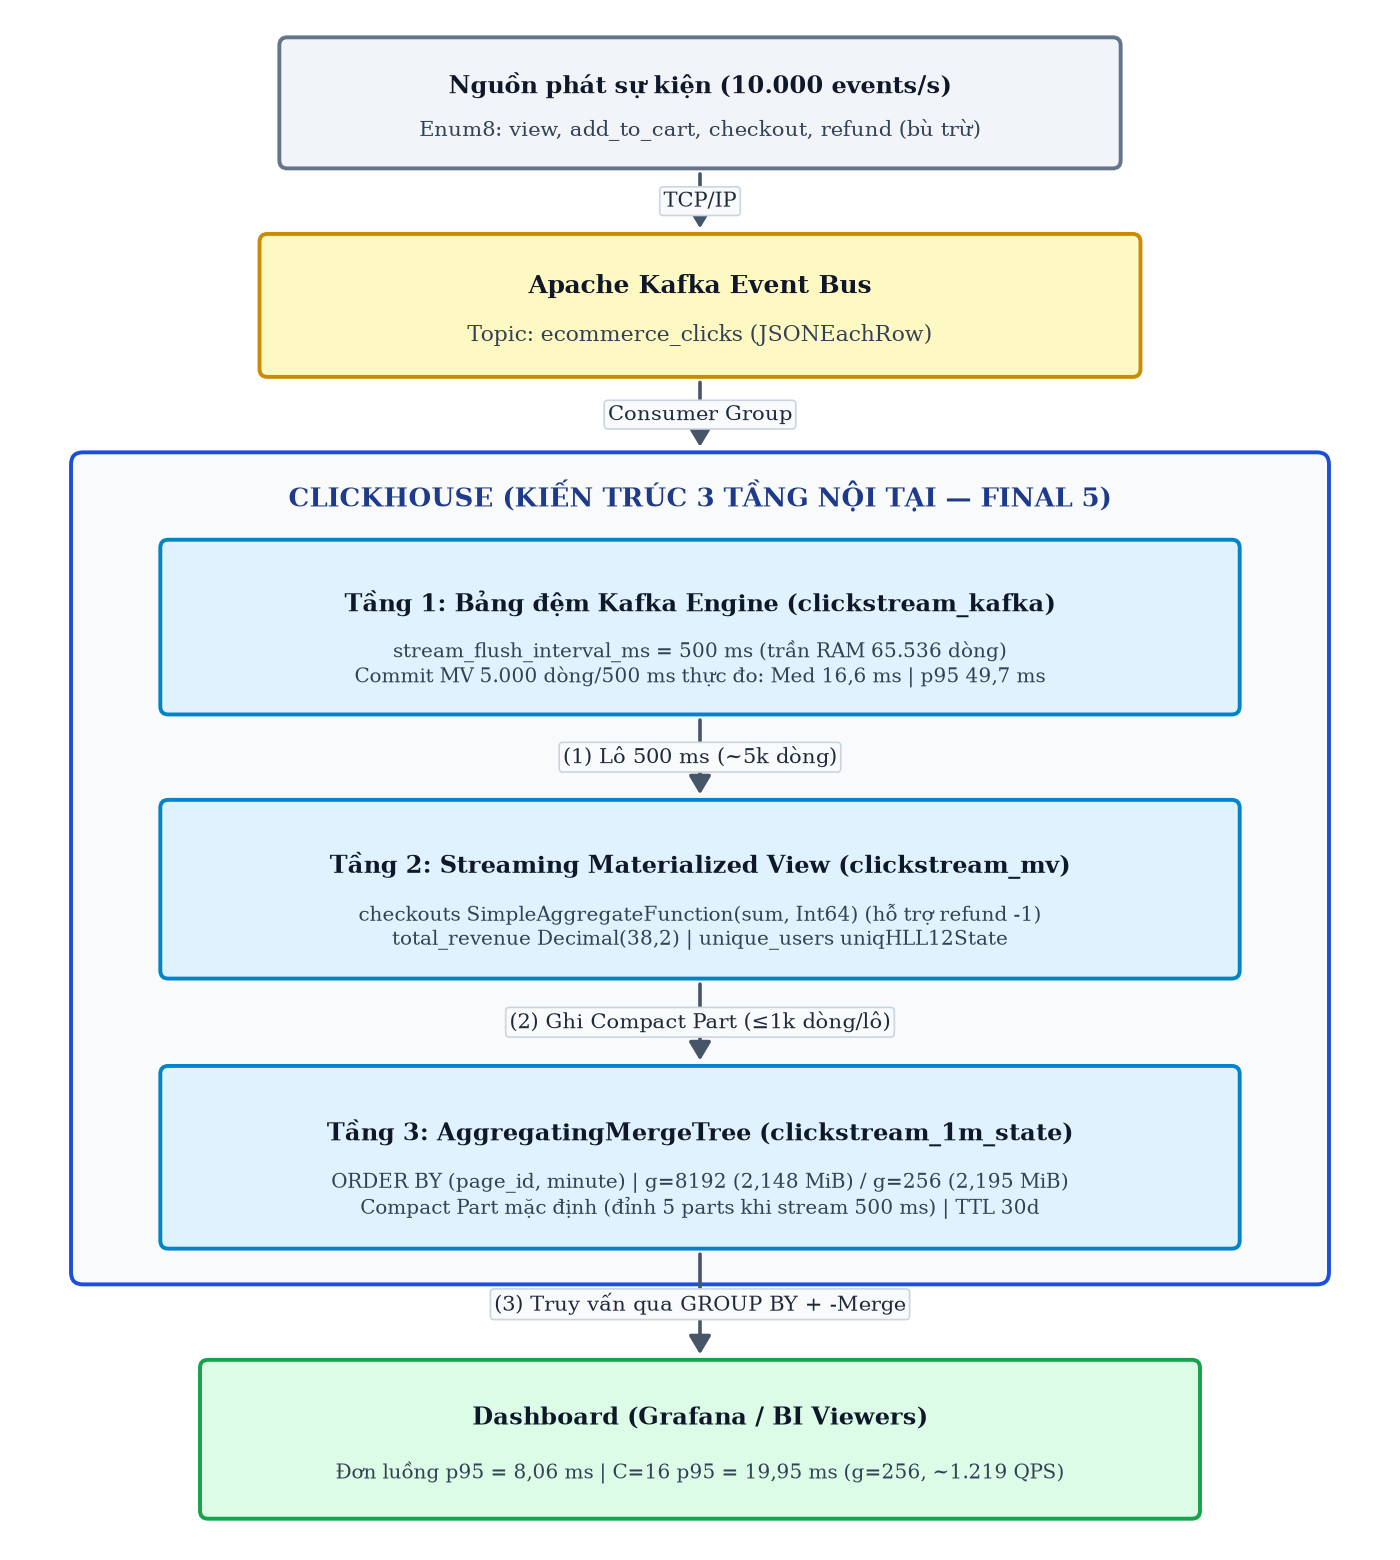
\includegraphics[width=0.86\textwidth,height=0.34\textheight,keepaspectratio]{fig5_1.png}
    }{
        \fbox{\parbox{0.9\textwidth}{\centering\vspace{0.8cm}\textbf{[Chèn Hình 5.1 -- tệp \texttt{fig5\_\allowbreak{}1.png}]}\vspace{0.8cm}}}
    }
    \caption[Kiến trúc luồng 3 tầng xử lý Clickstream thời gian thực trong ClickHouse]{Sơ đồ kiến trúc luồng dữ liệu 3 tầng xử lý Clickstream thời gian thực nội tại trong ClickHouse (cập nhật kiểu \texttt{total\_checkouts Int64}, sự kiện \texttt{refund}, $g = 256$ và thông số PoC máy chủ thực tế).}
    \label{fig:fig5_1}
\end{figure}

\subsection{Cơ chế 3~tầng: Kafka Flush 500~ms, Monoidal Sketch \& Tinh chỉnh vật lý MergeTree}
\begin{enumerate}
    \setlength{\itemsep}{2pt}\setlength{\parskip}{0pt}
    \item \textbf{Tầng~1 --- Cân bằng cỡ lô E3 và SLO $< 1{,}5~\text{s}$:} Chờ \texttt{kafka\_\allowbreak{}max\_\allowbreak{}block\_\allowbreak{}size = 65536} tại 10k/s mất tới 6,55~giây. Cần giữ 65.536 làm trần bảo vệ RAM nhưng đặt \texttt{stream\_\allowbreak{}flush\_\allowbreak{}interval\_\allowbreak{}ms = 500} (chu kỳ xả thực tế thay vì mặc định 7.500~ms; lưu ý \texttt{kafka\_\allowbreak{}poll\_\allowbreak{}timeout\_\allowbreak{}ms} chỉ là timeout đọc socket) trên profile ingest để gom $\approx 5.000$~sự kiện mỗi 0,5~s trong RAM, rồi qua MV thu gọn xuống $\le 1.000$~dòng trạng thái trước khi chạm đĩa.
    \item \textbf{Tầng~2 --- Monoidal Sketch \& Khắc phục bẫy \texttt{UInt64} cho \texttt{refund}:} Streaming MV vận hành như \textit{insert trigger} trên từng khối~\cite{S14}. Thay vì \texttt{UInt64} không chứa được số âm, lược đồ dùng \texttt{SimpleAggregateFunction(sum, Int64)} cho \texttt{total\_\allowbreak{}checkouts} (\texttt{+1} cho \texttt{'checkout'}, \texttt{-1} cho \texttt{'refund'}) đồng bộ với \texttt{Decimal(38, 2)} cho doanh thu; riêng \texttt{COUNT(\allowbreak{}DISTINCT user\_\allowbreak{}id)} dùng \texttt{AggregateFunction(\allowbreak{}uniqHLL12, UInt64)} ($m = 4.096$ thanh ghi, $\approx 2{,}59~\text{KiB/dòng}$, sai số chuẩn $\approx 1{,}04/\sqrt{4.096} \approx 1{,}6\%$~\cite{A3, V3}) có tính chất Monoid $S_{A \cup B}[j] = \max(S_A[j], S_B[j])$ hợp nhất tuyến tính mọi part.
    \item \textbf{Tầng~3 --- Bộ ba tinh chỉnh MergeTree (E1--E3):} (i)~\textbf{\texttt{ORDER BY (page\_\allowbreak{}id, minute)}} gom phác thảo HLL cùng trang cạnh nhau, nén cột HLL 105,6${\times}$ (còn 1,437~MiB; cả bảng $40{,}32 \rightarrow 2{,}148~\text{MiB}$) và hạ $p_{95}$ từ 136,48 về 8,06~ms; (ii)~giữ mặc định \textbf{Compact Part} (\texttt{10~MiB}) gom gọn 7~cột vào 1~\texttt{data.bin}; và (iii)~do cột HLL nặng $\approx 2{,}59~\text{KiB/dòng}$, hạ \textbf{\texttt{index\_\allowbreak{}granularity = 256}} co lượng đọc xuống 512~dòng (57,9~KiB, giảm 14,4${\times}$ so với 4.096~dòng Adaptive ở $g=8.192$), nâng trần thông lượng lên 1.219,2~QPS mà chỉ tốn thêm 48~KiB đĩa (+2,2\%) và 944~B RAM, kèm \texttt{DoubleDelta/\allowbreak{}T64+ZSTD(1)} và \texttt{TTL + 30 DAY}~\cite{S15, S16}.
\end{enumerate}

\subsection{Triển khai kỹ thuật (Mã DDL \& Query tối ưu)}
\begin{tcolorbox}[sqlblock]
\setlength{\topsep}{0pt}\setlength{\partopsep}{0pt}\footnotesize\setstretch{1.03}
\begin{verbatim}
-- 1. TẦNG 1: KAFKA ENGINE (PROFILE ĐẶT stream_flush_interval_ms=500)
CREATE TABLE default.clickstream_kafka (
    event_time DateTime, user_id UInt64, page_id UInt32,
    event_type Enum8('view'=1,'add_to_cart'=2,'checkout'=3,'refund'=4),
    revenue    Decimal(18, 2)
) ENGINE = Kafka SETTINGS kafka_broker_list = 'kafka:9092',
    kafka_topic_list = 'ecommerce_clicks', kafka_format = 'JSONEachRow',
    kafka_group_name = 'ch_clickstream', kafka_max_block_size = 65536;

-- 2. TẦNG 3: BẢNG ĐÍCH AggregatingMergeTree (ORDER BY page_id, g=256)
CREATE TABLE default.clickstream_1m_state (
    minute             DateTime CODEC(DoubleDelta, ZSTD(1)),
    page_id            UInt32   CODEC(T64, ZSTD(1)),
    total_views        SimpleAggregateFunction(sum, UInt64),
    total_add_to_carts SimpleAggregateFunction(sum, UInt64),
    total_checkouts    SimpleAggregateFunction(sum, Int64),
    total_revenue      SimpleAggregateFunction(sum, Decimal(38, 2)),
    unique_users       AggregateFunction(uniqHLL12, UInt64)
) ENGINE = AggregatingMergeTree() PARTITION BY toYYYYMM(minute)
ORDER BY (page_id, minute) TTL minute + INTERVAL 30 DAY
SETTINGS index_granularity = 256;

-- 3. TẦNG 2: STREAMING MV GIA TĂNG & BÙ TRỪ REFUND
CREATE MATERIALIZED VIEW default.clickstream_mv
TO default.clickstream_1m_state AS
SELECT toStartOfMinute(event_time) AS minute, page_id,
    countIf(event_type = 'view')        AS total_views,
    countIf(event_type = 'add_to_cart') AS total_add_to_carts,
    sumIf(toInt64(1), event_type = 'checkout')
      + sumIf(toInt64(-1), event_type = 'refund') AS total_checkouts,
    sum(revenue) AS total_revenue, uniqHLL12State(user_id) AS unique_users
FROM default.clickstream_kafka GROUP BY minute, page_id;

-- 4. TRUY VẤN DASHBOARD (-Merge GỘP PART CHƯA MERGE Ở THỜI GIAN THỰC)
SELECT minute, sum(total_views) AS views,
    sum(total_add_to_carts) AS carts, sum(total_checkouts) AS net_orders,
    sum(total_revenue) AS net_rev, uniqHLL12Merge(unique_users) AS uu
FROM default.clickstream_1m_state
WHERE page_id = 42 AND minute >= now() - INTERVAL 1 HOUR
GROUP BY minute ORDER BY minute ASC;
\end{verbatim}
\end{tcolorbox}

\subsection{Chiến lược khử trùng lặp 2~chế độ khắc phục \texttt{SUM} không lũy đẳng}
Vì \texttt{uniqHLL12} có tính lũy đẳng nhưng \texttt{SUM} sẽ cộng đúp nếu lô sự kiện gửi lặp, kiến trúc bổ sung 2~lớp khử trùng: (1)~\textbf{chống lặp theo lô (\textit{Block-level Deduplication}, chi phí đọc bằng 0)} bằng mã băm 128-bit trên \texttt{ReplicatedMergeTree} (\texttt{insert\_\allowbreak{}deduplicate = 1})~\cite{V4}; và (2)~\textbf{khử trùng từng \texttt{event\_\allowbreak{}id}} bằng \texttt{ReplacingMergeTree(\allowbreak{}ingest\_\allowbreak{}ver)} riêng cho luồng tài chính (\texttt{checkout}/\texttt{refund}, chiếm $< 5\%$ lưu lượng) để giữ luồng Dashboard \texttt{view} luôn đạt $< 50~\text{ms}$ không phải trả chi phí \texttt{FINAL}~\cite{V1, P11}:

\begin{tcolorbox}[sqlblock]
\setlength{\topsep}{0pt}\setlength{\partopsep}{0pt}\footnotesize\setstretch{1.03}
\begin{verbatim}
CREATE TABLE default.financial_events_dedup (
    event_id UUID, event_time DateTime, page_id UInt32, user_id UInt64,
    event_type Enum8('checkout'=3, 'refund'=4), revenue Decimal(18, 2),
    ingest_ver UInt64
) ENGINE = ReplacingMergeTree(ingest_ver)
PARTITION BY toYYYYMM(event_time)
ORDER BY (toDate(event_time), page_id, event_id);
-- Đối soát: SELECT page_id, sum(revenue) FROM financial_events_dedup FINAL
\end{verbatim}
\end{tcolorbox}

\section{Kiểm chứng thực nghiệm PoC trên máy chủ ClickHouse 26.10.4.207}
Để kiểm chứng toàn diện giải pháp trong môi trường thực tế, nghiên cứu triển khai một thực thể máy chủ \texttt{clickhouse-server 26.10.4.207} cô lập qua giao thức HTTP (\texttt{127.0.0.1:18123}, bật \texttt{system.\allowbreak{}part\_\allowbreak{}log}, \texttt{query\_\allowbreak{}cache}, \texttt{max\_\allowbreak{}concurrent\_\allowbreak{}queries = 256}) để đo trọn vẹn 3~kịch bản: (1)~lưu trữ và truy vấn đơn luồng 36~triệu sự kiện; (2)~tải đọc đồng thời $C = 1\text{--}128$ kèm phân vị $p_{95}$/$p_{99}$; và (3)~mô phỏng luồng micro-batch \texttt{JSONEachRow} mỗi 500~ms dưới tải đọc song song.

\subsection{Đối chứng 36~triệu sự kiện (Bảng thô 12 cột vs 5 cột vs \texorpdfstring{\texttt{AggregatingMergeTree}}{AggregatingMergeTree})}
Dữ liệu giả lập gồm đúng 36.000.000~sự kiện (1~giờ tải 10.000~sự kiện/s, 60~phút, 1.000~mã trang \texttt{page\_\allowbreak{}id}, 200.000~\texttt{user\_\allowbreak{}id} phân biệt), sử dụng hàm băm độc lập \texttt{cityHash64(\allowbreak{}number, 1) \% 20} để bảo đảm mọi trang đều chứa đủ $\approx 80\%$~\texttt{view}, $\approx 15\%$~\texttt{add\_\allowbreak{}to\_\allowbreak{}cart} và $\approx 5\%$~\texttt{checkout} (cụ thể tại \texttt{page\_\allowbreak{}id = 42}: 28.719 \texttt{view}, 5.513 \texttt{add\_\allowbreak{}to\_\allowbreak{}cart}, 1.768 \texttt{checkout}, doanh thu 109.580,64). Thử nghiệm đo 2 warmup + 15 lượt chính thức ở \texttt{max\_\allowbreak{}threads = 4}, tắt cache (Bảng~\ref{tab:ch5_36m}).

\begin{table}[!htb]
\centering
\scriptsize
\caption[Kết quả thực đo PoC 36 triệu sự kiện trên máy chủ ClickHouse]{Kết quả thực đo PoC 36~triệu sự kiện (1 giờ tải) trên \texttt{clickhouse-server 26.10.4.207} (\texttt{max\_threads = 4}, $n = 15$, tắt cache)}
\label{tab:ch5_36m}
\resizebox{\textwidth}{!}{%
\begin{tabular}{lccccc}
\toprule
\textbf{Chỉ số thực đo} & \textbf{\begin{tabular}[c]{@{}c@{}}Bảng thô 12 cột\\(\texttt{tuple()})\end{tabular}} & \textbf{\begin{tabular}[c]{@{}c@{}}Bảng thô 5 cột\\(\texttt{event\_\allowbreak{}time, page\_\allowbreak{}id})\end{tabular}} & \textbf{\begin{tabular}[c]{@{}c@{}}Aggregating\\(\texttt{minute, page\_\allowbreak{}id}, $g=8.192$)\end{tabular}} & \textbf{\begin{tabular}[c]{@{}c@{}}Aggregating tối ưu\\(\texttt{page\_\allowbreak{}id, minute}, $g=8.192$)\end{tabular}} & \textbf{\begin{tabular}[c]{@{}c@{}}Aggregating $g=256$\\(\texttt{page\_\allowbreak{}id, minute})\end{tabular}} \\
\midrule
Số dòng lưu trữ / giờ & 36.000.000 & 36.000.000 & 60.000 & 60.000 & 60.000 \\
Dung lượng đĩa / giờ & 703,05~MiB & 287,94~MiB & 40,32~MiB & 2,148~MiB & 2,195~MiB \\
\texttt{read\_\allowbreak{}rows} (Dashboard) & 36.000.000 (0\%) & 31.047.680 (13,8\%) & 60.000 (0\%) & 4.096 (Adaptive) & 512 (2 marks) \\
\texttt{read\_\allowbreak{}bytes} logic & 602,55~MiB & 392,20~MiB & 11,90~MiB & 832,0~KiB & 57,9~KiB \\
Client Median (IQR) & 232,21~ms (2,50) & 285,65~ms (6,89) & 121,97~ms (0,99) & 7,68~ms (0,11) & 5,92~ms (0,32) \\
Client $p_{95}$ ($< 50$ ms) & 239,48~ms (Trượt) & 301,06~ms (Trượt) & 136,48~ms (Trượt) & 8,06~ms (Đạt) & 14,88~ms (Đạt) \\
Server Med / $p_{95}$ & 230,95 / 238,17~ms & 284,49 / 299,99~ms & 120,88 / 135,39~ms & 6,59 / 6,93~ms & --- \\
\bottomrule
\end{tabular}%
}
\end{table}

\noindent\textit{(Giải trình Bảng~\ref{tab:ch5_36m}: [1]~\texttt{clickstream\_\allowbreak{}1m\_\allowbreak{}state} [2,148~MiB] gọn hơn bảng thô 12~cột [703,05~MiB, chưa nén $\approx 1.422{,}1~\text{MB}$ sau \texttt{SerializationSparse}] tới 327${\times}$; [2]~bảng thô 5~cột nhảy khối rời rạc chậm hơn quét tuần tự [285,65 vs 232,21~ms]; [3]~mức \texttt{read\_\allowbreak{}bytes} chỉ còn 832,0~KiB [$g=8.192$] và 57,9~KiB [$g=256$] dù cột HLL cả bảng nặng 159,06~MB là nhờ lọc hai pha \texttt{PREWHERE page\_\allowbreak{}id = 42} tự động bỏ qua giải nén cột HLL ngoài vùng trang 42; [4]~ở $g = 256$, $p_{95} = 14{,}88~\text{ms}$ trên $n=15$ bị kéo bởi 1~ngoại lệ, khi đo $n = 200$ tại Bảng~\ref{tab:ch5_concurrent} đạt $p_{95} = 6{,}38~\text{ms}$.)}

\subsection{Phân giải dung lượng theo cột, Sai số HLL12, Bù trừ \texorpdfstring{\texttt{refund}}{refund} và Gửi lặp}
Bảng~\ref{tab:ch5_columns} phân tích chi tiết mức nén từng cột trong bảng tổng hợp \texttt{clickstream\_\allowbreak{}1m\_\allowbreak{}state} ($g = 8.192$, trích từ \texttt{system.\allowbreak{}parts\_\allowbreak{}columns}) cùng 2~kiểm chứng nghiệp vụ quan trọng trên mã trang đại diện \texttt{page\_\allowbreak{}id = 42}:

\begin{table}[!ht]
\centering
\footnotesize
\renewcommand{\arraystretch}{1.15}
\caption[Dung lượng nén theo cột, sai số HLL12, refund và gửi lặp 5 phút]{Dung lượng nén theo cột (\texttt{system.parts\_columns}), sai số HLL12, kiểm chứng \texttt{refund} và gửi lặp 5 phút}
\label{tab:ch5_columns}
\setlength{\tabcolsep}{4pt}
\begin{tabularx}{\textwidth}{>{\bfseries\raggedright\arraybackslash}p{2.35cm} >{\raggedright\arraybackslash}p{3.55cm} >{\raggedright\arraybackslash}p{2.45cm} >{\raggedright\arraybackslash}p{2.85cm} >{\raggedright\arraybackslash}X}
\toprule
\textbf{Hạng mục / Phép kiểm chứng} & \textbf{Kiểu dữ liệu / Kịch bản} & \textbf{Trước / Giá trị chuẩn} & \textbf{Sau / Thực đo thực tế} & \textbf{Kết luận kỹ thuật} \\
\midrule
Cột \texttt{minute} & \texttt{DateTime}\newline(\texttt{DoubleDelta, ZSTD(1)}) & 240.000~B & 418~B ($\approx 574{\times}$) & Bước nhảy đều 60~s nén gần như tuyệt đối \\
\addlinespace[3pt]
5 cột khóa, đếm, tiền & \texttt{page\_\allowbreak{}id}, \texttt{total\_\allowbreak{}*},\newline \texttt{Decimal(38, 2)} & 2.640.000~B & 735.602~B ($\approx 718~\text{KiB}$) & Chiếm $\approx 32{,}8\%$ dung lượng bảng (4 hành vi thực không bị toàn 0) \\
\addlinespace[3pt]
Cột \texttt{unique\_\allowbreak{}users} & \texttt{AggregateFunction(}\newline\texttt{uniqHLL12, UInt64)} & 159.060.000~B & 1.506.638~B (1,437~MiB) & Nén 105,6${\times}$ nhờ \texttt{ORDER BY (page\_\allowbreak{}id, minute)} xếp cùng trang liền kề \\
\addlinespace[3pt]
Độ chính xác \texttt{uniqHLL12} & \texttt{page\_\allowbreak{}id = 42} / Toàn bộ 1.000 trang & 200 / 200.000 (\texttt{uniqExact}) & 202 (+1,00\%) / 201.514 (+0,76\%) & Nằm gọn trong biên sai số chuẩn lý thuyết $\approx 1{,}6\%$ \\
\addlinespace[3pt]
Kiểm chứng 3 giao dịch \texttt{refund} & Nạp 3 sự kiện \texttt{'refund'}, $-150{,}00$ (user đã mua) & $k = 1.768$; $\text{rev} = 109.580{,}64$; $u = 202$ & $k = 1.765$ ($-3$); $\text{rev} = 109.130{,}64$ ($-450{,}00$); $u = 202$ & Kiểu \texttt{Int64} + \texttt{'refund'} giảm đúng cả doanh thu và số đơn ròng; user giữ nguyên \\
\addlinespace[3pt]
Kiểm chứng gửi lặp 5 phút & Nạp trùng lô 5 phút đầu \texttt{page\_\allowbreak{}id = 42} & $\text{views} = 28.719$; $k = 1.765$; $\text{rev} = 109.130{,}64$; $u = 204$ (sau thêm 3 mã vãng lai) & $\text{views} = 31.099$ (+2.380); $k = 1.918$ (+153); $\text{rev} = 118.613{,}58$; $u = 204$ & HLL lũy đẳng ($\max(R, R) = R$), nhưng \texttt{SUM} KHÔNG lũy đẳng $\rightarrow$ cần dedup ở tầng nạp nếu yêu cầu chuẩn kế toán \\
\bottomrule
\end{tabularx}
\end{table}
\FloatBarrier

\noindent\textbf{Liên hệ kế thừa trực tiếp từ chuỗi thực nghiệm E1--E3:}
\begin{enumerate}
    \setlength{\itemsep}{3pt}\setlength{\parskip}{0pt}
    \item \textbf{Kế thừa E1 (\texttt{ORDER BY (page\_\allowbreak{}id, minute)}):} Chuyển tiền tố sang \texttt{page\_\allowbreak{}id} cắt \texttt{read\_\allowbreak{}rows} từ 60.000 xuống 4.096 (93,2\%), kéo $p_{95}$ từ 136,48~ms về 8,06~ms, nén riêng cột HLL tới 105,6${\times}$ (từ 159,06~MB còn 1,437~MiB) và thu gọn tổng dung lượng bảng 18,8${\times}$ ($40{,}32 \rightarrow 2{,}148~\text{MiB}$).
    \item \textbf{Kế thừa E2 (Khắc phục tác động kích thước dòng lớn):} Ngược với bảng hẹp 44~B ở E2, mỗi dòng của \texttt{clickstream\_\allowbreak{}1m\_\allowbreak{}state} nặng $\approx 2{,}64~\text{KiB}$ (2.699~B thô), nên ngưỡng mặc định \texttt{index\_\allowbreak{}granularity\_\allowbreak{}bytes = 10~MiB} tự động kích hoạt \textit{Adaptive Granularity} cắt đôi hạt xuống còn 4.096~dòng (\texttt{marks = 16}, \texttt{pk\_\allowbreak{}mem = 64~B}). Chủ động hạ tiếp xuống $g = 256$ giảm \texttt{read\_\allowbreak{}rows} xuống 512~dòng (\texttt{pk\_\allowbreak{}mem = 944~B}), giải phóng cổ chai CPU giải nén HLL ở tải đồng thời cao.
    \item \textbf{Kế thừa E3 (Tiền tổng hợp MV + Compact Part):} Thu gọn lượng dòng chạm đĩa 600${\times}$ ($36\text{M} \rightarrow 60\text{k}$), kết hợp thử nghiệm nhánh \texttt{state\_\allowbreak{}g256} xác nhận HLL giữ nguyên $202 \rightarrow 202$ sau 3 lệnh \texttt{refund}, tăng đúng $+2$ lên 204 khi thêm 3 lượt xem khách mới rồi giữ bất biến $204 \rightarrow 204$ sau khi gửi trùng toàn bộ lô 5~phút.
    \item \textbf{Cộng hưởng mã hóa chuyên biệt (\texttt{DoubleDelta}, \texttt{T64} và nén HLL):} Trong bảng tổng hợp 60.000~dòng, cột thời gian \texttt{minute} tăng đều 60~s đạt tỷ số nén $\approx 574{\times}$ (240.000~B còn 418~B) dưới bộ mã hóa \texttt{DoubleDelta + ZSTD(1)}, trong khi thanh ghi \texttt{unique\_\allowbreak{}users} (\texttt{uniqHLL12}, bản thô 159,06~MB) giảm gấp 105,6${\times}$ xuống còn 1,437~MiB khi các dòng cùng \texttt{page\_\allowbreak{}id} được gom sát nhau theo khóa sắp xếp; đồng thời trong quá trình quét 1~trang, tầng tối ưu hai pha \texttt{PREWHERE} lọc bỏ toàn bộ cột HLL ngoài 2~marks mục tiêu giúp giữ lượng giải nén ở mức 57,9~KiB~\cite{S16, A3}.
\end{enumerate}

\subsection{Thử nghiệm tải đọc đồng thời HTTP (\texorpdfstring{$C = 1\text{--}128$}{C = 1..128}) và tối ưu \texorpdfstring{$g = 256$}{g = 256}}
Để kiểm chứng cam kết ``$p_{95} < 50~\text{ms}$ dưới tải đồng thời'', nhóm dùng bộ sinh tải HTTP đa luồng (\texttt{http.\allowbreak{}client} giữ kết nối, truy vấn ngẫu nhiên đều trên 1.000~\texttt{page\_\allowbreak{}id}, $n = 200\text{--}1.280$ lượt/mức, lỗi 0\%) đánh giá $g = 8.192$ và $g = 256$ (Bảng~\ref{tab:ch5_concurrent}, Hình~\ref{fig:fig5_2}a). Lưu ý ở phép đo đồng thời này, \texttt{max\_\allowbreak{}threads} được hạ chủ động từ 4 (ở Mục~5.3.1 đơn luồng) xuống \texttt{2} nhằm tránh tranh chấp quá tải luồng CPU (\textit{thread oversubscription}) trên máy chủ 8~nhân khi hàng chục truy vấn chạy song song.

\begin{table}[!htb]
\centering
\footnotesize
\caption{Hiệu năng Dashboard HTTP đồng thời trên máy chủ \texttt{clickhouse-server 26.10.4.207} (8 nhân, tắt Cache là mặc định kiểm chuẩn)}
\label{tab:ch5_concurrent}
\resizebox{\textwidth}{!}{%
\begin{tabular}{lccccccp{4.3cm}}
\toprule
\textbf{Cấu hình \& Cache} & \textbf{\begin{tabular}[c]{@{}c@{}}Số kết nối\\song song ($C$)\end{tabular}} & \textbf{\begin{tabular}[c]{@{}c@{}}Tổng lượt\\đo ($n$)\end{tabular}} & \textbf{\begin{tabular}[c]{@{}c@{}}Median\\(ms)\end{tabular}} & \textbf{\begin{tabular}[c]{@{}c@{}}$p_{95}$\\(ms)\end{tabular}} & \textbf{\begin{tabular}[c]{@{}c@{}}$p_{99}$\\(ms)\end{tabular}} & \textbf{\begin{tabular}[c]{@{}c@{}}Thông lượng\\(QPS)\end{tabular}} & \textbf{Đánh giá SLO $p_{95} < 50$ ms} \\
\midrule
$g = 8.192$ (Cache TẮT) & 1 & 200 & 7,28 & 8,25 & 8,74 & 138,5 & Đạt \\
$g = 8.192$ (Cache TẮT) & 16 & 640 & 15,72 & 25,69 & 33,15 & 942,4 & Đạt \\
$g = 8.192$ (Cache TẮT) & 64 & 1.280 & 57,51 & 104,37 & 146,49 & 956,3 (Bão hòa) & Vượt SLO (nghẽn CPU HLL) \\
$g = 8.192$ (Cache TẮT) & 128 & 1.280 & 86,44 & 194,71 & 252,52 & 956,2 (Bão hòa) & Vượt SLO (hàng đợi HTTP) \\
$g = 8.192$ (Cache BẬT 5s) & 128 ($\approx 22\%$~hit) & 1.280 & 80,74 & 180,20 & 229,91 & 1.009,1 & Giảm nhẹ do phân tán 1k trang \\
\midrule
$g = 256$ (Cache TẮT) & 1 & 200 & 5,65 & 6,38 & 7,73 & 170,2 & Đạt (Cải thiện 23\%) \\
$g = 256$ (Cache TẮT) & 16 & 640 & 12,13 & 19,95 & 35,50 & 1.175,1 & Đạt (Nhanh hơn 22\%) \\
$g = 256$ (Cache TẮT) & 64 & 1.280 & 40,63 & 83,07 & 102,97 & 1.188,9 & Med đạt, $p_{95}$ vượt nhẹ \\
$g = 256$ (Cache TẮT) & 128 & 1.280 & 37,99 & 79,44 & 100,33 & 1.219,2 & Med đạt, $p_{95}$ giảm $2{,}45{\times}$ so với $g = 8.192$ \\
\bottomrule
\end{tabular}%
}
\end{table}

\noindent\textbf{Nhận định kỹ thuật trung thực từ Bảng~\ref{tab:ch5_concurrent}:}
\begin{itemize}
    \setlength{\itemsep}{2pt}\setlength{\parskip}{0pt}
    \item Trên 1~nút 8~nhân tắt Query Cache và phân bố đều 1.000~trang lạnh, $g = 8.192$ bão hòa CPU giải nén+HLL tại $\approx 956~\text{QPS}$; hạ $g = 256$ (giảm 14,4${\times}$ đọc HLL) nâng trần lên \textbf{1.219,2~QPS} (+27,5\%) và rút $p_{95}$ tại $C = 128$ xuống \textbf{79,44~ms} (2,45${\times}$ nhanh hơn; lưu ý $C / \text{QPS} = 104{,}99~\text{ms} > p_{99}$ do khoảng 1\% truy vấn đuôi chịu chờ hàng đợi + đồng bộ client).
    \item Tại $\le 16$ kết nối đồng thời, cả $g=256$ ($p_{95} = 19{,}95~\text{ms}$) và $g=8.192$ ($25{,}69~\text{ms}$) đều đạt sâu dưới SLO $< 50~\text{ms}$, đủ phục vụ hàng trăm người dùng làm mới định kỳ 5~giây + Query Cache trang nóng; để phục vụ $C = 64\text{--}128$ truy vấn lạnh cùng tích tắc dưới 50~ms cần nhân bản read-replica.
\end{itemize}

\subsection{Thử nghiệm luồng micro-batch \texorpdfstring{\texttt{JSONEachRow}}{JSONEachRow} mỗi 500~ms dưới 16 luồng đọc song song}
Để kiểm chứng ảnh hưởng thực sự của cơ chế xả \texttt{stream\_\allowbreak{}flush\_\allowbreak{}interval\_\allowbreak{}ms = 500} ms lên độ tươi mới dữ liệu, áp lực gộp part và đọc đồng thời, nhóm thiết lập bảng \texttt{ENGINE = Null} nối qua Streaming MV sang \texttt{clickstream\_\allowbreak{}1m\_\allowbreak{}state} và phát liên tiếp 30 micro-batch \texttt{JSONEachRow} (5.000 sự kiện/lô = 10.000~sự kiện/giây thực tế trong 15 giây = 150.000 sự kiện), đồng thời cho 16 luồng Dashboard đọc liên tục không tắt nghỉ trên chính bảng đích đó (Bảng~\ref{tab:ch5_stream}, Hình~\ref{fig:fig5_2}b). \textit{(Giới hạn phạm vi PoC: bài thử phát 30 micro-batch HTTP \texttt{JSONEachRow} trong 15 giây trực tiếp vào Null + MV chỉ kiểm chứng pha xử lý Streaming MV và merge nền ngắn hạn trước ngưỡng chuyển Wide Part 10~MiB --- chưa bao gồm chi phí Kafka Broker/consumer thật cũng như thử nghiệm độ bền nhiều giờ qua ngưỡng nâng cấp Compact $\rightarrow$ Wide).}

\begin{table}[!htb]
\centering
\scriptsize
\renewcommand{\arraystretch}{1.15}
\caption{Kết quả luồng micro-batch 500~ms qua Streaming MV dưới 16 luồng đọc song song (Compact mặc định vs Wide)}
\label{tab:ch5_stream}
\begin{tabularx}{\textwidth}{>{\bfseries\raggedright\arraybackslash}p{3.4cm} >{\raggedright\arraybackslash}p{3.1cm} >{\raggedright\arraybackslash}p{3.1cm} >{\raggedright\arraybackslash}X}
\toprule
\textbf{Chỉ số đo đạc (15~s phát liên tục, 16~luồng đọc)} & \textbf{Cấu hình chuẩn: Compact Part (\texttt{min\_\allowbreak{}bytes\_\allowbreak{}for\_\allowbreak{}wide\_\allowbreak{}part = 10~MiB})} & \textbf{Phản mẫu: Ép Wide Part (\texttt{min\_\allowbreak{}bytes\_\allowbreak{}for\_\allowbreak{}wide\_\allowbreak{}part = 0~B})} & \textbf{Ý nghĩa kỹ thuật} \\
\midrule
Commit MV mỗi lô 5k JSON: $p_{50}$ / $p_{95}$ (max) & 16,55 / 49,72~ms (74,39) & 17,02 / 46,20~ms (75,98) & Đóng góp DB vào độ tươi mới chỉ $\approx 17\text{--}50~\text{ms}$, cùng 500~ms flush nằm gọn dưới 1,5~s \\
\addlinespace
Tổng số truy vấn đọc phục vụ đồng thời (15~s) & 16.795 truy vấn & 15.105 truy vấn & Compact Part giữ thông lượng đọc cao hơn +11,2\% \\
\addlinespace
Độ trễ đọc Dashboard song song: $p_{50}$ / $p_{95}$ & 13,87 / 21,37~ms & 15,15 / 25,96~ms & Đọc đồng thời khi đang stream \& merge vẫn đạt sâu dưới SLO $< 50$ ms \\
\addlinespace
Số \texttt{NewPart} sinh ra $\rightarrow$ Đỉnh / Cuối active parts & 30~$\rightarrow$ Đỉnh~5 / Sau 2~s: 5 (5~Compact) & 30~$\rightarrow$ Đỉnh~5 / Sau 2~s: 5 (5~Wide) & Trong cửa sổ thử nghiệm 15~s (30 batch), merge nền giữ ổn định ở 5 parts, không có dấu hiệu tích tụ parts \\
\addlinespace
Hoạt động merge nền (\texttt{system.\allowbreak{}part\_\allowbreak{}log}) & 5 merges / 93~ms / 30.000 \texttt{read\_\allowbreak{}rows} & 5 merges / 99~ms / 30.000 \texttt{read\_\allowbreak{}rows} & Tỷ lệ $\Sigma r / N_{\text{raw}} = 30.000 / 150.000 = 0{,}200$ (rất thấp so với 4,517 ở E3!) \\
\addlinespace
Dung lượng và phân mảnh tệp sau stream & 341.594~B (chỉ 5 tệp \texttt{data.bin}) & 343.710~B (gấp 7${\times}$ số tệp cột) & Xác nhận lý do tránh đặt \texttt{min\_\allowbreak{}bytes\_\allowbreak{}for\_\allowbreak{}wide\_\allowbreak{}part = 0} cho các lô nhỏ \\
\bottomrule
\end{tabularx}
\end{table}

\begin{figure}[!htb]
    \centering
    \IfFileExists{fig5_2.png}{
        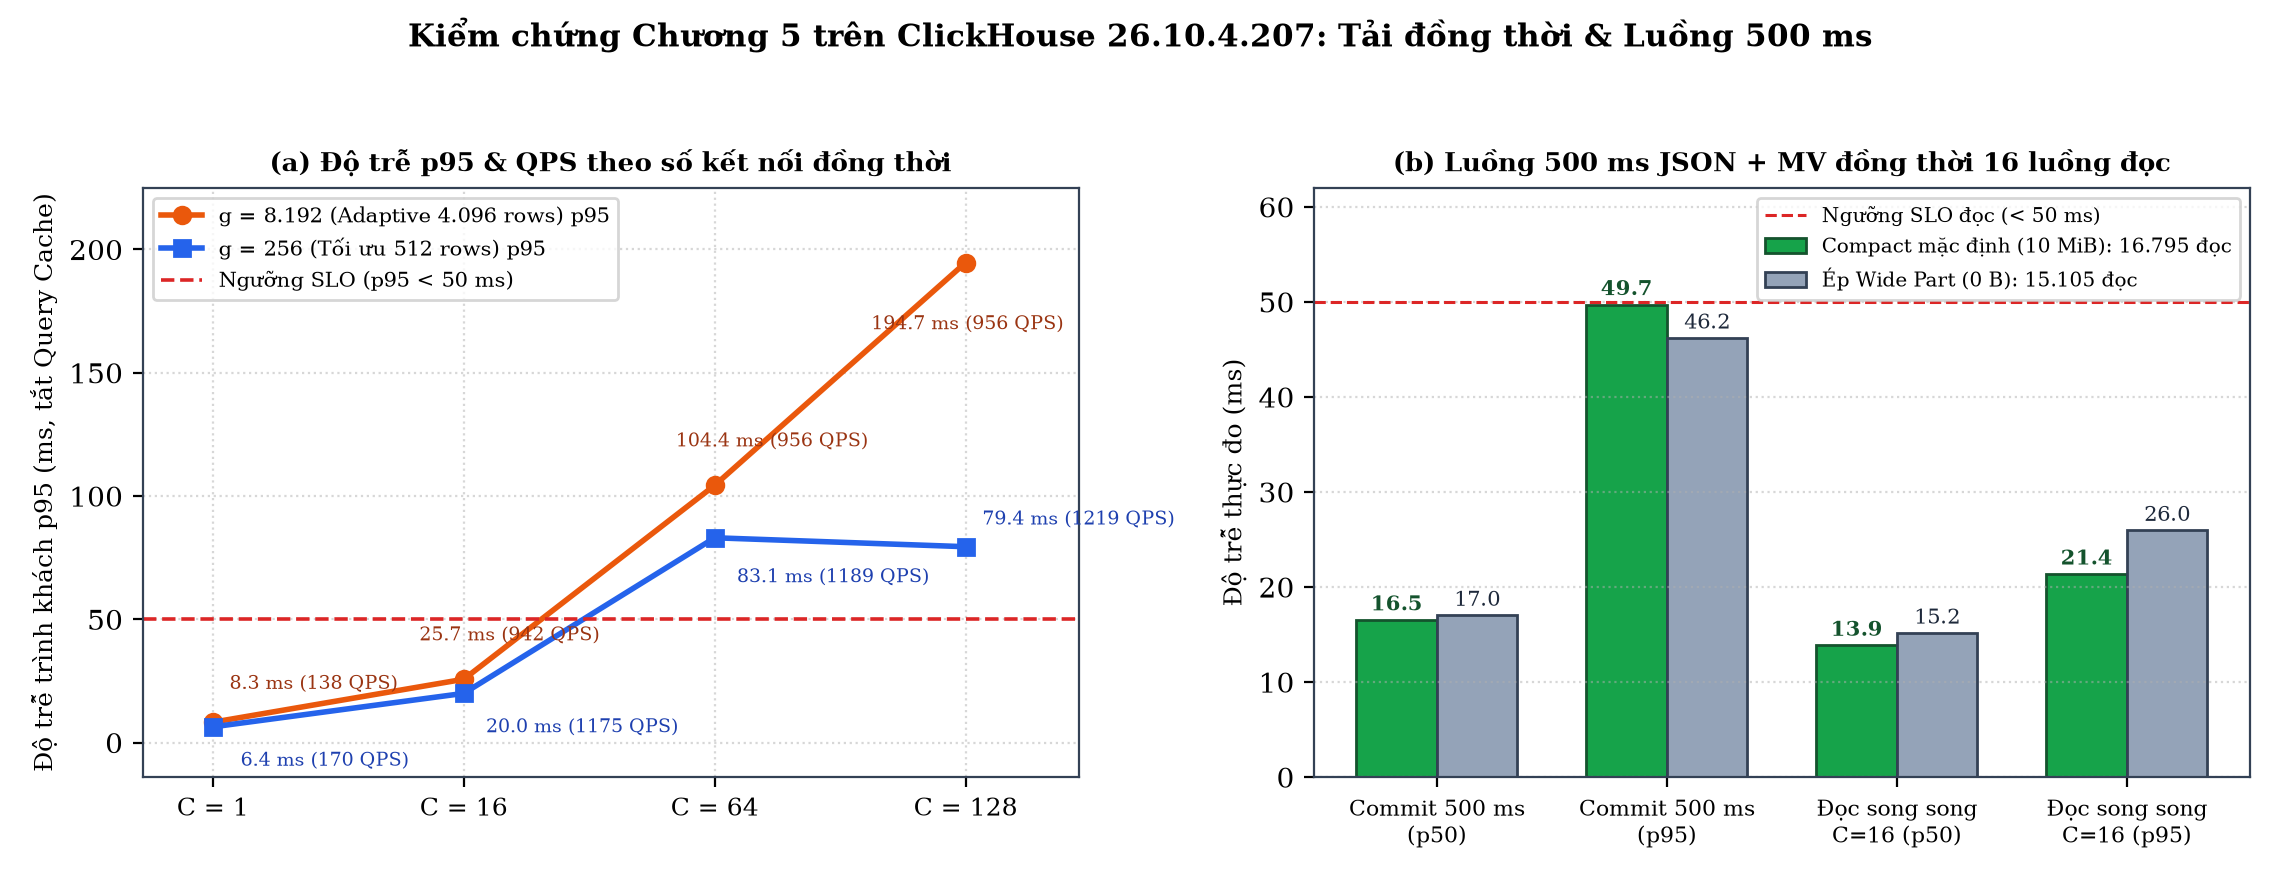
\includegraphics[width=0.94\textwidth,height=0.32\textheight,keepaspectratio]{fig5_2.png}
    }{
        \fbox{\parbox{0.9\textwidth}{\centering\vspace{0.8cm}\textbf{[Chèn Hình 5.2 -- tệp \texttt{fig5\_\allowbreak{}2.png}]}\vspace{0.8cm}}}
    }
    \caption{Kết quả kiểm chứng máy chủ \texttt{clickhouse-server 26.10.4.207} tại Chương 5: (a) Độ trễ $p_{95}$ \& thông lượng QPS ở tải đồng thời $C = 1\text{--}128$ ($g = 8.192$ vs $g = 256$); (b) Luồng \texttt{JSONEachRow} chu kỳ 500~ms qua Streaming MV dưới tải 16 luồng đọc song song (Compact vs Wide).}
    \label{fig:fig5_2}
\end{figure}

\subsection{Mở rộng kiểm chứng PoC: Hợp nhất Wide Part đồng thời và Chi phí \texttt{FINAL} 5\%}
Để thu hẹp khoảng cách kiểm chứng pha chuyển trạng thái dài hạn và tính chi phí lớp khử trùng tài chính trên chính \texttt{clickhouse-server 26.10.4.207} (\texttt{laptop1}), nhóm thực hiện hai phép đo bổ sung~\cite{M6}:
\begin{itemize}
    \setlength{\itemsep}{2pt}\setlength{\parskip}{0pt}
    \item \textbf{Hợp nhất nền Wide Part 77,57~MiB song song với 16 luồng đọc \& stream \texttt{Compact Part}:} Nạp sẵn 5~giờ dữ liệu (300.000~dòng HLL ở 5~Wide part $\approx 15{,}65~\text{MiB/part}$) rồi tiếp tục phát 20~micro-batch \texttt{JSONEachRow} (5.000~sự kiện/lô, \texttt{Compact Part} 26~KiB) qua \texttt{Null + MV} trong lúc 16~luồng đọc liên tục thực hiện \textbf{8.831~truy vấn} Dashboard (tắt Query Cache, \texttt{max\_\allowbreak{}threads = 2}). Kết quả trong \texttt{system.\allowbreak{}part\_\allowbreak{}log} ghi nhận merge nền gộp cả 5~Wide part thành 1~Wide part \textbf{77,57~MiB} (81.339.708~B, chạy 3.991~ms) và 3~Compact merge đồng thời, nhưng phía đọc vẫn đạt \textbf{$p_{50} = 19{,}82~\text{ms}$}, \textbf{$p_{95} = 35{,}67~\text{ms} < 50~\text{ms}$} và \textbf{$p_{99} = 46{,}11~\text{ms} < 50~\text{ms}$} nhờ cơ chế Part-level MVCC không khóa lẫn nhau.
    \item \textbf{Định lượng chi phí \texttt{ReplacingMergeTree FINAL} trên luồng tài chính 5\%:} Nạp 1.800.000~giao dịch \texttt{checkout}/\texttt{refund} (ứng 5\% của 36M~sự kiện/giờ, chia 2~part chưa merge tổng 40,93~MiB, cố ý chứa 26~mã \texttt{event\_\allowbreak{}id} trùng lặp) vào bảng \texttt{financial\_\allowbreak{}events\_\allowbreak{}dedup}. Đo 10~lượt ấm cho thấy truy vấn theo trang \texttt{WHERE page\_\allowbreak{}id = 42} dùng \texttt{FINAL} đạt trung vị \textbf{9,98~ms} ($p_{95} = 10{,}81~\text{ms}$), chỉ nhỉnh hơn không \texttt{FINAL} (8,53~ms) đúng \textbf{+1,45~ms}; còn quét đối soát toàn bộ 1,8M~dòng với \texttt{FINAL} mất \textbf{51,12~ms} ($p_{95} = 94{,}22~\text{ms}$) và lọc chính xác 1.800.000 $\rightarrow$ 1.799.974 bản ghi duy nhất.
\end{itemize}

\section{Tình huống biên, Kiến trúc lai \& Ranh giới PoC vs. Mở rộng}
\begin{itemize}
    \setlength{\itemsep}{3pt}\setlength{\parskip}{0pt}
    \item \textbf{Dữ liệu đến muộn và Bù trừ giao dịch hoàn tiền:} Các bản ghi sự kiện từ thiết bị mất mạng gửi muộn nhiều giờ vẫn tự động định tuyến chính xác vào phân vùng tháng quá khứ nhờ \texttt{PARTITION BY toYYYYMM(\allowbreak{}minute)}, đồng thời sự kiện \texttt{'refund'} mang số âm trừ đồng bộ cả \texttt{net\_\allowbreak{}checkouts} (\texttt{Int64}) lẫn \texttt{net\_\allowbreak{}revenue} (\texttt{page\_\allowbreak{}id = 42}: $1.768 \rightarrow 1.765$) mà không cần đột biến phân đoạn cũ.
    \item \textbf{Kiến trúc lai chuẩn công nghiệp (Hình~\ref{fig:fig5_3}):} \textbf{PostgreSQL} đảm nhận nguồn sự thật ACID (tài khoản, giỏ hàng, trạng thái đơn) và tra cứu điểm W3; tầng chuyển tiếp \textbf{Debezium CDC + Kafka}~\cite{P11} bắt thay đổi WAL PostgreSQL cùng luồng sự kiện trình duyệt; còn \textbf{ClickHouse} gánh trọn tải phân tích tổng hợp và Dashboard thời gian thực.
\end{itemize}

\begin{figure}[!htb]
    \centering
    \IfFileExists{fig5_3.png}{
        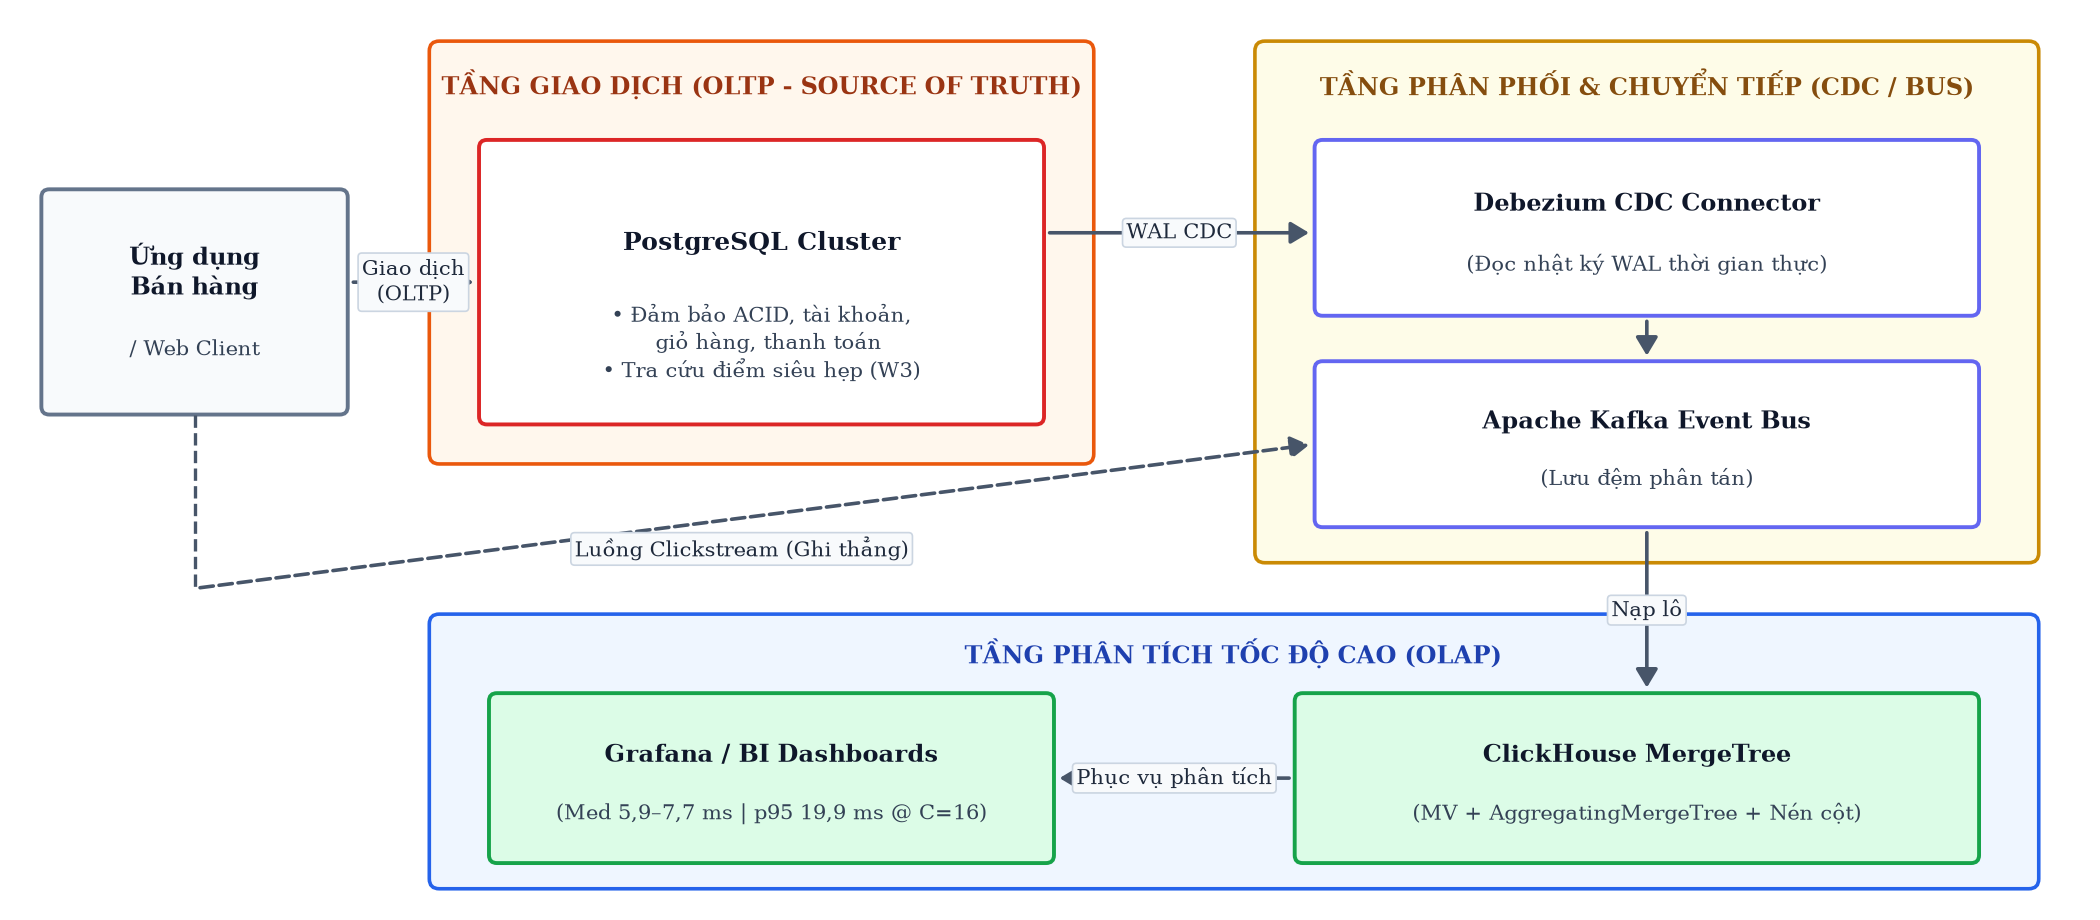
\includegraphics[width=0.88\textwidth,height=0.29\textheight,keepaspectratio]{fig5_3.png}
    }{
        \fbox{\parbox{0.9\textwidth}{\centering\vspace{0.5cm}\textbf{[Chèn Hình 5.3 -- tệp \texttt{fig5\_\allowbreak{}3.png}]}\vspace{0.5cm}}}
    }
    \caption[Mô hình kiến trúc lai hiện đại kết hợp PostgreSQL và ClickHouse]{Mô hình kiến trúc lai hiện đại kết hợp giữa PostgreSQL (OLTP) và ClickHouse (OLAP; lưu ý ở tải PoC $C=16$, $p_{95} = 19{,}95~\text{ms}$, hộp sơ đồ làm tròn 19,9~ms).}
    \label{fig:fig5_3}
\end{figure}

\needspace{5\baselineskip}
\noindent\textbf{Tổng hợp định lượng Trước -- Sau tối ưu và Khuyến nghị tham số:}
So sánh xuyên suốt chuỗi kiểm chứng PoC trên \texttt{clickhouse-server 26.10.4.207} cho thấy hiệu ứng cộng hưởng khi phối hợp đúng cả 3~điểm sáng MergeTree: chuyển từ \textbf{Bảng thô 12 cột (\texttt{tuple()})} sang \textbf{\texttt{AggregatingMergeTree} chưa tối ưu (\texttt{minute, page\_\allowbreak{}id})} mới chỉ giảm độ trễ trung vị từ 232,21~ms xuống 121,97~ms ($p_{95} = 136{,}48~\text{ms}$, vẫn trượt SLO $50~\text{ms}$ gần $3{\times}$); nhưng khi đảo khóa sang \textbf{\texttt{ORDER BY (page\_\allowbreak{}id, minute)}} và tinh chỉnh \textbf{$g = 256$}, dung lượng đĩa mỗi giờ rơi từ 703,05~MiB xuống \textbf{2,195~MiB} (nén $320{\times}$), lượng \texttt{read\_\allowbreak{}bytes} tụt từ 602,55~MiB xuống \textbf{57,9~KiB}, độ trễ đơn luồng đạt \textbf{5,92~ms} ($39{,}2{\times}$ nhanh hơn bảng thô), thông lượng bão hòa tăng lên \textbf{1.219,2~QPS}, còn khi phát stream 500~ms với Compact Part giữ $p_{95}$ đồng thời ở \textbf{21,37~ms} ($\Sigma r / N_{\text{raw}} = 0{,}200$) và ngay cả lúc merge Wide Part 77,57~MiB song song vẫn giữ $p_{95} = 35{,}67~\text{ms}$. Bức tranh này khẳng định bài học kỹ thuật then chốt: chỉ dùng Materialized View là chưa đủ nếu không đặt đúng tiền tố \texttt{ORDER BY} và kích thước hạt \texttt{index\_\allowbreak{}granularity} tương ứng độ rộng trạng thái HLL.

\needspace{6\baselineskip}
\noindent\textbf{Phân biệt rạch ròi Thực nghiệm PoC vs. Thiết kế Mở rộng:} Phép đo thực tế trên \texttt{clickhouse-server 26.10.4.207} chứng minh giải pháp chạy với bảng \texttt{Null + Streaming MV + AggregatingMergeTree + ReplacingMergeTree} (kèm kiểm chứng merge Wide Part 77,57~MiB đồng thời và \texttt{FINAL} 5\% chỉ tăng +1,45~ms ở Mục~5.3.5), đạt $p_{95} = 19{,}95~\text{ms} < 50~\text{ms}$ tới $C = 16$ kết nối không cache và giữ $p_{95} = 21{,}37~\text{ms}$ xuyên suốt 16.795 truy vấn khi stream micro-batch 500~ms ($\Sigma r / N_{\text{raw}} = 0{,}200$). Trong khi đó, kết nối Kafka Broker thật, tầng Debezium CDC, xác thực cụm \texttt{ReplicatedMergeTree} (\texttt{insert\_\allowbreak{}deduplicate=1}) và mở rộng ngang qua read-replica để đáp ứng $C = 64\text{--}128$ truy vấn không cache dưới $50~\text{ms}$ vẫn là phần \textit{thiết kế kiến trúc mở rộng} chưa triển khai cụm thực tế.

\needspace{6\baselineskip}
\section{Hạn chế và Khuyến nghị các trường hợp KHÔNG NÊN sử dụng ClickHouse}
Để bảo đảm tính khách quan kỹ thuật, cần tránh dùng ClickHouse trong 5~kịch bản sau:
\begin{enumerate}
    \setlength{\itemsep}{3pt}\setlength{\parskip}{0pt}
    \item \textbf{Giao dịch tài chính ACID đa dòng / đa bảng (OLTP thuần túy):} ClickHouse chỉ nguyên tử cấp từng Data Part khi chèn lô; thiếu khóa mức dòng, 2PC hay \texttt{ROLLBACK} $\Rightarrow$ dùng PostgreSQL/MySQL/Oracle.
    \item \textbf{Cập nhật hoặc xóa điểm tần suất cao:} Mutations (\texttt{ALTER TABLE ... UPDATE/\allowbreak{}DELETE}) buộc đọc, giải nén và ghi lại cả phân đoạn $\Rightarrow$ bão hòa I/O; trạng thái biến động nhanh nên đặt ở PostgreSQL/Redis.
    \item \textbf{Tra cứu bản ghi đơn lẻ siêu chọn lọc (\textit{Point-lookup}):} Khối nén 64~KiB--1~MiB và hạt chỉ mục thưa khiến W3 thua B-tree (5,56 vs 1,16~ms) $\Rightarrow$ dùng B-tree hoặc key--value store.
    \item \textbf{JOIN phức tạp trên nhiều bảng lớn:} Hash Join mặc định nạp bảng bên phải vào RAM dễ gây tràn bộ nhớ (OOM) và thiếu CBO đảo thứ tự nối $\Rightarrow$ ưu tiên Star Schema hoặc làm phẳng trước khi nạp.
    \item \textbf{Tập dữ liệu nhỏ (dưới vài triệu dòng):} Chi phí khởi tạo AST, điều phối luồng và giải nén khiến ClickHouse không nhanh hơn rõ rệt so với DuckDB/PostgreSQL trong khi vận hành phức tạp hơn.
\end{enumerate}

\chapter*{KẾT LUẬN CHUNG}
\phantomsection
\addcontentsline{toc}{chapter}{Kết luận chung}
\markboth{KẾT LUẬN CHUNG}{KẾT LUẬN CHUNG}

Báo cáo đã hoàn chỉnh bức tranh toàn diện về hệ quản trị cơ sở dữ liệu \textbf{ClickHouse} từ kiến trúc nền tảng, giải phẫu điểm sáng \textbf{MergeTree}, thực nghiệm kiểm soát tham số, đối chứng với cả PostgreSQL và DuckDB đến thiết kế giải pháp và kiểm chứng PoC thời gian thực qua 4~đóng góp chính:

\begin{enumerate}
    \setlength{\itemsep}{3pt}
    \setlength{\parskip}{0pt}
    \setlength{\parsep}{0pt}
    \item \textbf{Giới thiệu DBMS mới \& Giải phẫu điểm sáng MergeTree (Chương 1--3):} Bên cạnh kiến trúc DBMS đầy đủ (Push-based Vectorized \texttt{QueryPipeline}, \texttt{PREWHERE}, Part-level MVCC, External Spill và Keeper Raft), MergeTree khẳng định bản sắc qua phân đoạn cột bất biến, chỉ mục chính thưa \texttt{primary.idx} (21.978~B RAM), tuần tự hóa thưa (\texttt{SerializationSparse}) và hợp nhất nền liên tục. Chuỗi thực nghiệm có kiểm soát (E1--E3) cùng kiểm chứng mở rộng cho thấy khóa \texttt{ORDER BY} quyết định giải thuật cắt tỉa (99,95\%, tăng tốc $7{,}76{\times}$, $p = 0{,}00002$); mốc $g = 8.192$ cân bằng tối ưu trên bảng hẹp 44~B ($p \ge 0{,}121$); gom lô lớn triệt tiêu $\Sigma r / N$ từ 4,517 xuống 1,000 ($p = 0{,}00014$); Projection giải quyết W4 còn 7,30~ms ($6{,}90{\times}$); còn External Spill bảo vệ OOM và hoàn tất 10M \texttt{GROUP BY} với 144,70~MiB RAM.

    \item \textbf{Đối chiếu đa hệ quản trị với PostgreSQL~18.6 \& DuckDB~2.0.1 (Chương 1 \& 4):} Thực nghiệm đối chứng với PostgreSQL~18.6 xác nhận ClickHouse vượt trội $13{,}42{\times}\text{--}36{,}00{\times}$ ở quét tổng hợp/lọc cột phụ và gọn hơn 80,96\% dung lượng đĩa, còn PG2 B-tree thắng ở tra cứu điểm siêu hẹp (1,16 vs 5,56~ms, hòa vốn $\sim 20.000$ truy vấn). Khi đối chứng bổ sung cùng hệ cột trên \texttt{laptop1}, DuckDB~2.0.1 nhúng nội tiến trình nhanh hơn ở truy vấn đơn người dùng nóng RAM (3,23 vs 8,65~ms ở W1; 33,13 vs 52,96~ms ở W4, hòa ở W0 $p = 0{,}123$), trong khi ClickHouse nén đĩa gọn hơn 12,9\%--16,9\%, lật ngược W4 còn 7,30~ms với Projection và gánh đồng thời tải stream nhiều kết nối.

    \item \textbf{Ứng dụng giải quyết bài toán thực tế Clickstream 10k~events/s (Chương 5):} Áp dụng đồng bộ 3~điểm sáng MergeTree (\texttt{ORDER BY (page\_\allowbreak{}id, minute)}, tinh chỉnh $g = 256$ cho cột HLL 2,59~KiB/dòng, và \texttt{Compact Part} + Streaming MV 500~ms) cho thấy giải pháp đạt SLO $< 50~\text{ms}$ tới $C = 16$ kết nối không cache ($p_{95} = 19{,}95~\text{ms}$, trần 1.219,2~QPS), giữ đọc song song $p_{95} = 21{,}37~\text{ms}$ khi stream và $35{,}67~\text{ms}$ ngay cả lúc merge Wide Part 77,57~MiB, đồng thời xử lý bù trừ \texttt{refund} và khử trùng 2~tầng (\texttt{FINAL} 5\% chỉ thêm +1,45~ms).

    \item \textbf{Tính minh bạch khoa học và Định hướng triển khai sản xuất:} Toàn bộ kết quả tách bạch rạch ròi giữa số đo thực tế trên môi trường 1~nút (đối chiếu qua SHA-256, \texttt{EXPLAIN} và \texttt{system.\allowbreak{}query\_\allowbreak{}log}/\texttt{part\_\allowbreak{}log}) với các phần thiết kế kiến trúc mở rộng cụm chưa kiểm tải đa máy, làm cơ sở vững chắc để phân tuyến khối lượng công việc trong kiến trúc lai OLTP--OLAP.
\end{enumerate}

\noindent\textbf{Hướng mở rộng thực tế tiếp theo:}
\begin{enumerate}
    \setlength{\itemsep}{2pt}\setlength{\parskip}{0pt}
    \item Triển khai cụm \texttt{ReplicatedMergeTree} + Apache Kafka + Debezium CDC trên nhiều máy để đo độ trễ đầu-cuối ($p_{95}/p_{99}$) và xác thực \texttt{insert\_\allowbreak{}deduplicate=1} trên cụm phân tán~\cite{S17, V4, P11}.
    \item Thực nghiệm đối chứng trực tiếp PostgreSQL BRIN kết hợp \texttt{CLUSTER} định kỳ cùng Apache Druid trên tải hỗn hợp đọc--ghi và tính kiểm định Mann--Whitney~U đầy đủ từ log thô \texttt{crossdb-v3} của Chương~4.
    \item Kiểm chứng ngoại suy ngoài mẫu cho mô hình hồi quy pha nạp E3 ở các cỡ lô trung gian $B = 250\text{k}/500\text{k}$ kèm đo lường mức tiêu thụ RAM và băng thông ghi SSD đỉnh trong quá trình hợp nhất nền.
\end{enumerate}

\begin{thebibliography}{99}
\small
\setstretch{1.02}
\setlength{\parskip}{0pt}
\setlength{\itemsep}{1.5pt}

\item[] \hspace{-\leftmargin}\textbf{I. Công bố khoa học và tài liệu học thuật nền tảng}

\bibitem[A1]{A1} R. Schulze, T. Schreiber, I. Yatsishin, R. Dahimene, and A. Milovidov, ``ClickHouse - Lightning Fast Analytics for Everyone,'' \textit{Proceedings of the VLDB Endowment (PVLDB)}, vol. 17, no. 12, pp. 3731--3744, 2024. DOI: 10.14778/3685800.3685802. Available: \url{https://www.vldb.org/pvldb/vol17/p3731-schulze.pdf}

\bibitem[A2]{A2} D. Abadi, P. Boncz, S. Harizopoulos, S. Idreos, and S. Madden, ``The Design and Implementation of Modern Column-Oriented Database Systems,'' \textit{Foundations and Trends in Databases}, vol. 5, no. 3, pp. 197--280, 2013. DOI: 10.1561/1900000024.

\bibitem[A3]{A3} P. Flajolet, \'E. Fusy, O. Gandouet, and F. Meunier, ``HyperLogLog: the analysis of a near-optimal cardinality estimation algorithm,'' \textit{Proc. Conference on Analysis of Algorithms (AofA 07)}, 2007.

\bibitem[A4]{A4} A. Milovidov, ``Evolution of ClickHouse Architecture,'' \textit{ClickHouse Technical Presentations}, 2021. Available: \url{https://clickhouse.com/presentations}

\item[] \hspace{-\leftmargin}\textbf{II. Báo cáo kỹ thuật công nghiệp và bộ chuẩn đánh giá (Benchmark)}

\bibitem[B1]{B1} M. Vavrusa and M. Majkowski, ``HTTP Analytics for 6M requests per second using ClickHouse,'' \textit{Cloudflare Technical Blog}, 2018. Available: \url{https://blog.cloudflare.com/http-analytics-for-6m-requests-per-second-using-clickhouse/}

\bibitem[B2]{B2} X. Wang et al., ``Fast and Reliable Schema-Agnostic Log Analytics Platform (Migrating from ELK to ClickHouse),'' \textit{Uber Engineering Blog}, 2021. Available: \url{https://www.uber.com/blog/logging/}

\bibitem[B3]{B3} B. Giard, ``Financial Market Analytics at Scale with ClickHouse,'' \textit{Bloomberg Engineering Reports}, 2022. Available: \url{https://www.bloomberg.com/company/stories/}

\bibitem[B4]{B4} ClickHouse, Inc., ``ClickBench --- A Benchmark for Analytical DBMS,'' \textit{GitHub Repository}. Available: \url{https://github.com/ClickHouse/ClickBench}

\bibitem[B5]{B5} ClickHouse, Inc., ``ClickBench Schema (\texttt{clickhouse/create.sql}, commit \texttt{b0b7dd8f}),'' \textit{GitHub}. Available: \url{https://github.com/ClickHouse/ClickBench/blob/b0b7dd8f11a2a719211cc41d8c7ebbada267df66/clickhouse/create.sql}

\item[] \hspace{-\leftmargin}\textbf{III. Tài liệu kỹ thuật chính thức và mã nguồn ClickHouse}

\bibitem[S1]{S1} ClickHouse, Inc., ``ClickHouse Official Documentation: Architecture Overview \& MergeTree Engine Family,'' 2026. Available: \url{https://clickhouse.com/docs}

\bibitem[S2]{S2} ClickHouse, Inc., ``MergeTree Table Engine,'' \textit{ClickHouse Documentation}. Available: \url{https://clickhouse.com/docs/reference/engines/table-engines/mergetree-family/mergetree}

\bibitem[S3]{S3} ClickHouse, Inc., ``Data Parts,'' \textit{ClickHouse Documentation}. Available: \url{https://clickhouse.com/docs/concepts/core-concepts/parts}

\bibitem[S4]{S4} ClickHouse, Inc., ``Primary Indexes,'' \textit{ClickHouse Documentation}. Available: \url{https://clickhouse.com/docs/concepts/core-concepts/primary-indexes}

\bibitem[S4a]{S4a} ClickHouse, Inc., ``A Practical Introduction to Primary Indexes in ClickHouse,'' \textit{ClickHouse Documentation}. Available: \url{https://clickhouse.com/docs/guides/clickhouse/data-modelling/sparse-primary-indexes}

\bibitem[S5]{S5} ClickHouse, Inc., ``Part Merges'' (kèm minh họa Replacing merges, CC BY-NC-SA 4.0), \textit{ClickHouse Documentation}. Available: \url{https://clickhouse.com/docs/concepts/core-concepts/merges}

\bibitem[S6]{S6} ClickHouse, Inc., ``System Table: \texttt{system.parts},'' \textit{ClickHouse Documentation}. Available: \url{https://clickhouse.com/docs/reference/system-tables/parts}

\bibitem[S7]{S7} ClickHouse, Inc., ``EXPLAIN Statement,'' \textit{ClickHouse Documentation}. Available: \url{https://clickhouse.com/docs/reference/statements/explain}

\bibitem[S8]{S8} ClickHouse, Inc., ``System Table: \texttt{system.part\_log},'' \textit{ClickHouse Documentation}. Available: \url{https://clickhouse.com/docs/reference/system-tables/part_log}

\bibitem[S9]{S9} ClickHouse, Inc., ``Selecting an Insert Strategy'' (CC BY-NC-SA 4.0), \textit{ClickHouse Documentation}. Available: \url{https://clickhouse.com/docs/concepts/best-practices/selecting-an-insert-strategy}

\bibitem[S10]{S10} ClickHouse, Inc., ``System Table: \texttt{system.query\_log},'' \textit{ClickHouse Documentation}. Available: \url{https://clickhouse.com/docs/reference/system-tables/query_log}

\bibitem[S11]{S11} ClickHouse, Inc., ``System Table: \texttt{system.merges},'' \textit{ClickHouse Documentation}. Available: \url{https://clickhouse.com/docs/reference/system-tables/merges}

\bibitem[S12]{S12} ClickHouse, Inc., ``Avoiding \texttt{OPTIMIZE FINAL},'' \textit{ClickHouse Documentation}. Available: \url{https://clickhouse.com/docs/concepts/best-practices/avoid-optimize-final}

\bibitem[S13]{S13} ClickHouse, Inc., ``ClickHouse Source Code --- \texttt{MergeTreeSettings.cpp} (v26.10.3.7-stable),'' \textit{GitHub}. Available: \url{https://github.com/ClickHouse/ClickHouse/blob/v26.10.3.7-stable/src/Storages/MergeTree/MergeTreeSettings.cpp#L2701-L2714}

\bibitem[S14]{S14} ClickHouse, Inc., ``Incremental Materialized Views,'' \textit{ClickHouse Documentation}. Available: \url{https://clickhouse.com/docs/concepts/features/materialized-views/incremental-materialized-view}

\bibitem[S15]{S15} ClickHouse, Inc., ``TTL (Time To Live) for Columns and Tables,'' \textit{ClickHouse Documentation}. Available: \url{https://clickhouse.com/docs/concepts/features/operations/delete/ttl}

\bibitem[S16]{S16} ClickHouse, Inc., ``Column Compression Codecs (\texttt{CODEC}),'' \textit{ClickHouse Documentation}. Available: \url{https://clickhouse.com/docs/reference/statements/create/table/codec}

\bibitem[S17]{S17} ClickHouse, Inc., ``Shards and Replicas,'' \textit{ClickHouse Documentation}. Available: \url{https://clickhouse.com/docs/guides/oss/deployment-and-scaling/shards}

\bibitem[S18]{S18} ClickHouse, Inc., ``RowBinary Input and Output Format,'' \textit{ClickHouse Documentation}. Available: \url{https://clickhouse.com/docs/reference/formats/RowBinary/RowBinary}

\bibitem[S19]{S19} ClickHouse, Inc., ``OPTIMIZE Statement,'' \textit{ClickHouse Documentation}. Available: \url{https://clickhouse.com/docs/reference/statements/optimize}

\bibitem[V1]{V1} ClickHouse, Inc., ``ReplacingMergeTree Table Engine,'' \textit{ClickHouse Documentation}. Available: \url{https://clickhouse.com/docs/reference/engines/table-engines/mergetree-family/replacingmergetree}

\bibitem[V2]{V2} ClickHouse, Inc., ``SummingMergeTree Table Engine,'' \textit{ClickHouse Documentation}. Available: \url{https://clickhouse.com/docs/reference/engines/table-engines/mergetree-family/summingmergetree}

\bibitem[V3]{V3} ClickHouse, Inc., ``AggregatingMergeTree Table Engine,'' \textit{ClickHouse Documentation}. Available: \url{https://clickhouse.com/docs/reference/engines/table-engines/mergetree-family/aggregatingmergetree}

\bibitem[V4]{V4} ClickHouse, Inc., ``Data Replication,'' \textit{ClickHouse Documentation}. Available: \url{https://clickhouse.com/docs/reference/engines/table-engines/mergetree-family/replication}

\item[] \hspace{-\leftmargin}\textbf{IV. Tài liệu kỹ thuật chính thức PostgreSQL 18 và Tích hợp CDC}

\bibitem[P1]{P1} PostgreSQL Global Development Group, ``Chapter 66. Database Physical Storage --- Database Page Layout,'' \textit{PostgreSQL 18 Documentation}. Available: \url{https://www.postgresql.org/docs/18/storage-page-layout.html}

\bibitem[P2]{P2} PostgreSQL Global Development Group, ``Chapter 65. BRIN Indexes,'' \textit{PostgreSQL 18 Documentation}. Available: \url{https://www.postgresql.org/docs/18/brin.html}

\bibitem[P3]{P3} PostgreSQL Global Development Group, ``Chapter 11.2. Index Types (B-tree),'' \textit{PostgreSQL 18 Documentation}. Available: \url{https://www.postgresql.org/docs/18/indexes-types.html}

\bibitem[P4]{P4} PostgreSQL Global Development Group, ``Chapter 11.3. Multicolumn Indexes,'' \textit{PostgreSQL 18 Documentation}. Available: \url{https://www.postgresql.org/docs/18/indexes-multicolumn.html}

\bibitem[P5]{P5} PostgreSQL Global Development Group, ``SQL Command: CLUSTER,'' \textit{PostgreSQL 18 Documentation}. Available: \url{https://www.postgresql.org/docs/18/sql-cluster.html}

\bibitem[P6]{P6} PostgreSQL Global Development Group, ``SQL Command: VACUUM,'' \textit{PostgreSQL 18 Documentation}. Available: \url{https://www.postgresql.org/docs/18/sql-vacuum.html}

\bibitem[P7]{P7} PostgreSQL Global Development Group, ``SQL Command: ANALYZE,'' \textit{PostgreSQL 18 Documentation}. Available: \url{https://www.postgresql.org/docs/18/sql-analyze.html}

\bibitem[P8]{P8} PostgreSQL Global Development Group, ``Write Ahead Log (WAL) Runtime Configuration,'' \textit{PostgreSQL 18 Documentation}. Available: \url{https://www.postgresql.org/docs/18/runtime-config-wal.html}

\bibitem[P9]{P9} PostgreSQL Global Development Group, ``Using EXPLAIN,'' \textit{PostgreSQL 18 Documentation}. Available: \url{https://www.postgresql.org/docs/18/using-explain.html}

\bibitem[P10]{P10} PostgreSQL Global Development Group, ``Database Object Size Functions,'' \textit{PostgreSQL 18 Documentation}. Available: \url{https://www.postgresql.org/docs/18/functions-admin.html#FUNCTIONS-ADMIN-DBOBJECT}

\bibitem[P11]{P11} Debezium Community, ``Debezium Connector for PostgreSQL Reference Documentation.'' Available: \url{https://debezium.io/documentation/reference/stable/connectors/postgresql.html}

\item[] \hspace{-\leftmargin}\textbf{V. Tiêu chuẩn đo lường, thuật toán nén và Kho dữ liệu tái lập}

\bibitem[M1]{M1} LZ4 Project, ``LZ4 --- Extremely Fast Compression Algorithm.'' Available: \url{https://lz4.org/}

\bibitem[M2]{M2} NIST/SEMATECH, ``Measures of Scale (Standard Deviation),'' \textit{e-Handbook of Statistical Methods}. Available: \url{https://www.itl.nist.gov/div898/handbook/eda/section3/eda356.htm}

\bibitem[M3]{M3} NIST, ``Coefficient of Variation,'' \textit{Dataplot Reference Manual}. Available: \url{https://www.itl.nist.gov/div898/software/dataplot/refman2/auxillar/coefvari.htm}

\bibitem[M4]{M4} NIST, ``Prefixes for Binary Multiples,'' \textit{The NIST Reference on Constants, Units, and Uncertainty}. Available: \url{https://physics.nist.gov/cuu/Units/binary.html}

\bibitem[M5]{M5} NIST, ``Secure Hash Standard (SHS) --- FIPS PUB 180-4.'' Available: \url{https://csrc.nist.gov/pubs/fips/180-4/upd1/final}

\bibitem[M6]{M6} Nhóm nghiên cứu (\texttt{INT3202\_I\_GROUP\_8}), ``Kho mã nguồn chính thức, kịch bản thực nghiệm và cấu hình giao thức (\texttt{clickhouse-mergetree-study} / \texttt{INT3202\_I\_GROUP\_8\_ClickHouseRepo}),'' \textit{GitHub Repository}. Available: \url{https://github.com/w1ndS0ng/clickhouse-mergetree-study}

\bibitem[M7]{M7} Nhóm nghiên cứu, ``Hồ sơ log, số đo và đối chứng E1 (\texttt{laptop1}), E2 (\texttt{wsl\_xeon}), E3 (\texttt{laptop\_i5}: \texttt{e3\_three\_runs\_20261117}) và Chương 4 (\texttt{formal43\_v3\_20261123}, \texttt{formal30m\_i5\_20261124\_105023}),'' \textit{GitHub Repository Branches} (\texttt{ha/sorting-key}, \texttt{tuan/granularity}, \texttt{tai/batch-merge}, \texttt{tai/e3-run-20261117}).

\end{thebibliography}

% -------------------- PHỤ LỤC A --------------------
\appendix
\titleformat{\chapter}[block]
  {\normalfont\bfseries\Large\centering}{PHỤ LỤC \thechapter.}{0.5em}{}

\chapter{BẢNG GIẢI THÍCH NGUỒN GỐC TỪNG HÌNH ẢNH}

Toàn bộ 14~hình trong báo cáo không sử dụng công cụ AI tạo ảnh (\textit{generative image AI}) ở bất kỳ hình nào: 3 hình kết quả thực nghiệm chính thức (Hình 3.1, Hình 3.2, Hình 5.2) được vẽ tự động bằng Matplotlib (Python) từ log CSV/JSON thực đo của ClickHouse; 3 hình sơ đồ kiến trúc Chương 2 (Hình 2.1--2.3) được dựng từ mã mô tả sơ đồ vector kỹ thuật, 2 hình kiến trúc Chương 5 (Hình 5.1, 5.3) cùng biểu đồ đối chiếu (Hình 3.3) được dựng bằng mã nguồn Matplotlib vector 200 dpi từ tài liệu kỹ thuật và số đo gốc; 3 hình (Hình 2.4--2.6) là minh họa sư phạm 16 dòng giả định do nhóm tự dựng; và 2 hình (Hình 2.7--2.8) trích nguyên bản từ ClickHouse Docs theo giấy phép mở CC BY-NC-SA 4.0.

\begin{table}[!htb]
\centering
\footnotesize
\renewcommand{\arraystretch}{1.15}
\caption{Nguồn gốc, công cụ tạo lập và dữ liệu đối chiếu của toàn bộ 14~hình trong báo cáo}
\label{tab:appendix_figures}
\begin{tabularx}{\textwidth}{>{\bfseries\raggedright\arraybackslash}p{2.25cm} >{\raggedright\arraybackslash}p{5.55cm} >{\raggedright\arraybackslash}X}
\toprule
\textbf{Hình} & \textbf{Công cụ / Cách tạo ra} & \textbf{Nguồn kiến thức / Nguồn số liệu sử dụng trong hình} \\
\midrule
Hình 2.1, 2.2, 2.3 & Sơ đồ khối dựng bằng mã vector thuần và kết xuất thành PNG độ phân giải cao (không dùng AI tạo ảnh). & Sơ đồ lý thuyết kiến trúc, không chứa số đo thực nghiệm. Nội dung tổng hợp từ bài báo VLDB 2024~\cite{A1} và tài liệu chính thức ClickHouse~\cite{S2, S3, S4}. \\
\addlinespace
Hình 2.4 & Bảng minh họa cấu trúc vector dùng kiểu chữ có chân (Times) và tô màu nền theo trạng thái khớp điều kiện. & Ví dụ giả lập 16 bản ghi do nhóm tự thiết kế theo mục đích sư phạm (\texttt{CounterID} 100/200, ngày 15--18, 4~dòng/granule) để giải thích lý thuyết sắp xếp~\cite{S2, S4}. \\
\addlinespace
Hình 2.5, 2.6 & Hình vẽ vector thể hiện các ô chữ nhật và mũi tên chú thích. & Ví dụ giả lập 16 hàng ($g = 2$ vs $g = 8$) và sơ đồ minh họa hợp nhất Part A, B, C $\rightarrow$ D theo cơ chế của tài liệu ClickHouse~\cite{S2, S3, S4, S5}. \\
\addlinespace
Hình 2.7, 2.8 & Ảnh gốc trích từ Tài liệu chính thức ClickHouse (ClickHouse Docs). & Lấy từ hai trang hướng dẫn chính thức: \textit{Selecting an insert strategy}~\cite{S9} và \textit{Replacing merges}~\cite{S5, V1} (CC BY-NC-SA 4.0). \\
\addlinespace
Hình 3.1 & Vẽ tự động bằng mã Python (Matplotlib v3.11.2) qua hàm \texttt{plot(run)} trong \texttt{src/\allowbreak{}mtstudy/\allowbreak{}analysis.py}, xuất tại \texttt{artifacts/\allowbreak{}ha/\allowbreak{}laptop1/\allowbreak{}main01/\allowbreak{}figures/\allowbreak{}keys\_\allowbreak{}30m.png/\allowbreak{}.svg}. & Số liệu thực nghiệm thật 100\% (E1 trên \texttt{laptop1}) trích từ \texttt{summary/\allowbreak{}queries.csv} (150 lượt đo, xác nhận bởi \texttt{system.\allowbreak{}query\_\allowbreak{}log} và \texttt{explain/\allowbreak{}keys\_\allowbreak{}30m\_\allowbreak{}*.json}), khớp Bảng~\ref{tab:e1_results}. \\
\addlinespace
Hình 3.2 & Vẽ bằng Python (Matplotlib v3.11.2) theo bố cục 4 ô (\texttt{e2\_\allowbreak{}granularity\_\allowbreak{}tradeoff\_\allowbreak{}v5}) trong \texttt{src/\allowbreak{}mtstudy/\allowbreak{}analysis.py}. & Số liệu thực nghiệm thật 100\% (E2 trên \texttt{wsl\_\allowbreak{}xeon}, \texttt{e2main\_\allowbreak{}v2\_\allowbreak{}20261117}) từ \texttt{queries.csv} và \texttt{granularity\_\allowbreak{}cost.csv}, khớp Bảng~\ref{tab:e2_results} và Bảng~\ref{tab:e2_storage}. \\
\addlinespace
Hình 3.3 & Biểu đồ 2 ô kết xuất trực tiếp từ dữ liệu thực nghiệm (không dùng AI tạo ảnh). & Số liệu thực nghiệm thật 100\%: ô (a) lấy từ \texttt{estimated\_\allowbreak{}vs\_\allowbreak{}actual.csv} và \texttt{model.json} (E1 holdout 30M trên \texttt{laptop1}); ô (b) lấy từ \texttt{model\_\allowbreak{}and\_\allowbreak{}provenance.json} và \texttt{Trung\_\allowbreak{}binh\_\allowbreak{}3\_\allowbreak{}run\_\allowbreak{}3\_\allowbreak{}batch.csv} (E3 trên \texttt{laptop\_\allowbreak{}i5}). Khớp hoàn toàn Bảng~\ref{tab:e1_forecast} và Bảng~\ref{tab:e3_forecast}. \\
\addlinespace
Hình 5.1, 5.3 & Sơ đồ khối vector dựng từ mã nguồn Matplotlib (200 dpi, không dùng AI tạo ảnh). & Sơ đồ kiến trúc giải pháp Chương 5, kết hợp Kafka Engine (\texttt{stream\_\allowbreak{}flush\_\allowbreak{}interval\_\allowbreak{}ms = 500~ms}), MV (\texttt{total\_\allowbreak{}checkouts Int64}, \texttt{refund}), AggregatingMergeTree (\texttt{ORDER BY (page\_\allowbreak{}id, minute)}, $g = 256/8192$), Debezium CDC~\cite{P11} và các thông số thực đo máy chủ 26.10.4.207. \\
\addlinespace
Hình 5.2 & Biểu đồ 2 ô kết xuất trực tiếp bằng Matplotlib từ tệp log JSON thực nghiệm (200 dpi). & Số liệu thực đo 100\% trên thực thể cô lập \texttt{clickhouse-server 26.10.4.207} (\url{http://127.0.0.1:18123}): ô (a) tải HTTP đồng thời $C = 1\text{--}128$ ($g = 8.192$ vs $g = 256$); ô (b) luồng 500~ms \texttt{JSONEachRow} qua MV đồng thời 16 luồng đọc (Compact Part vs Wide Part). \\
\bottomrule
\end{tabularx}
\end{table}

\end{document}
